% Options for packages loaded elsewhere
\PassOptionsToPackage{unicode}{hyperref}
\PassOptionsToPackage{hyphens}{url}
\PassOptionsToPackage{dvipsnames,svgnames,x11names}{xcolor}
%
\documentclass[
  12pt,
  letterpaper,
  DIV=11,
  numbers=noendperiod]{scrartcl}

\usepackage{amsmath,amssymb}
\usepackage{setspace}
\usepackage{iftex}
\ifPDFTeX
  \usepackage[T1]{fontenc}
  \usepackage[utf8]{inputenc}
  \usepackage{textcomp} % provide euro and other symbols
\else % if luatex or xetex
  \usepackage{unicode-math}
  \defaultfontfeatures{Scale=MatchLowercase}
  \defaultfontfeatures[\rmfamily]{Ligatures=TeX,Scale=1}
\fi
\usepackage{lmodern}
\ifPDFTeX\else  
    % xetex/luatex font selection
\fi
% Use upquote if available, for straight quotes in verbatim environments
\IfFileExists{upquote.sty}{\usepackage{upquote}}{}
\IfFileExists{microtype.sty}{% use microtype if available
  \usepackage[]{microtype}
  \UseMicrotypeSet[protrusion]{basicmath} % disable protrusion for tt fonts
}{}
\makeatletter
\@ifundefined{KOMAClassName}{% if non-KOMA class
  \IfFileExists{parskip.sty}{%
    \usepackage{parskip}
  }{% else
    \setlength{\parindent}{0pt}
    \setlength{\parskip}{6pt plus 2pt minus 1pt}}
}{% if KOMA class
  \KOMAoptions{parskip=half}}
\makeatother
\usepackage{xcolor}
\setlength{\emergencystretch}{3em} % prevent overfull lines
\setcounter{secnumdepth}{-\maxdimen} % remove section numbering
% Make \paragraph and \subparagraph free-standing
\makeatletter
\ifx\paragraph\undefined\else
  \let\oldparagraph\paragraph
  \renewcommand{\paragraph}{
    \@ifstar
      \xxxParagraphStar
      \xxxParagraphNoStar
  }
  \newcommand{\xxxParagraphStar}[1]{\oldparagraph*{#1}\mbox{}}
  \newcommand{\xxxParagraphNoStar}[1]{\oldparagraph{#1}\mbox{}}
\fi
\ifx\subparagraph\undefined\else
  \let\oldsubparagraph\subparagraph
  \renewcommand{\subparagraph}{
    \@ifstar
      \xxxSubParagraphStar
      \xxxSubParagraphNoStar
  }
  \newcommand{\xxxSubParagraphStar}[1]{\oldsubparagraph*{#1}\mbox{}}
  \newcommand{\xxxSubParagraphNoStar}[1]{\oldsubparagraph{#1}\mbox{}}
\fi
\makeatother

\usepackage{color}
\usepackage{fancyvrb}
\newcommand{\VerbBar}{|}
\newcommand{\VERB}{\Verb[commandchars=\\\{\}]}
\DefineVerbatimEnvironment{Highlighting}{Verbatim}{commandchars=\\\{\}}
% Add ',fontsize=\small' for more characters per line
\usepackage{framed}
\definecolor{shadecolor}{RGB}{36,41,46}
\newenvironment{Shaded}{\begin{snugshade}}{\end{snugshade}}
\newcommand{\AlertTok}[1]{\textcolor[rgb]{1.00,0.33,0.33}{\textbf{#1}}}
\newcommand{\AnnotationTok}[1]{\textcolor[rgb]{0.42,0.45,0.49}{#1}}
\newcommand{\AttributeTok}[1]{\textcolor[rgb]{0.98,0.46,0.51}{#1}}
\newcommand{\BaseNTok}[1]{\textcolor[rgb]{0.47,0.72,1.00}{#1}}
\newcommand{\BuiltInTok}[1]{\textcolor[rgb]{0.98,0.46,0.51}{#1}}
\newcommand{\CharTok}[1]{\textcolor[rgb]{0.62,0.80,1.00}{#1}}
\newcommand{\CommentTok}[1]{\textcolor[rgb]{0.42,0.45,0.49}{#1}}
\newcommand{\CommentVarTok}[1]{\textcolor[rgb]{0.42,0.45,0.49}{#1}}
\newcommand{\ConstantTok}[1]{\textcolor[rgb]{0.47,0.72,1.00}{#1}}
\newcommand{\ControlFlowTok}[1]{\textcolor[rgb]{0.98,0.46,0.51}{#1}}
\newcommand{\DataTypeTok}[1]{\textcolor[rgb]{0.98,0.46,0.51}{#1}}
\newcommand{\DecValTok}[1]{\textcolor[rgb]{0.47,0.72,1.00}{#1}}
\newcommand{\DocumentationTok}[1]{\textcolor[rgb]{0.42,0.45,0.49}{#1}}
\newcommand{\ErrorTok}[1]{\textcolor[rgb]{1.00,0.33,0.33}{\underline{#1}}}
\newcommand{\ExtensionTok}[1]{\textcolor[rgb]{0.98,0.46,0.51}{\textbf{#1}}}
\newcommand{\FloatTok}[1]{\textcolor[rgb]{0.47,0.72,1.00}{#1}}
\newcommand{\FunctionTok}[1]{\textcolor[rgb]{0.70,0.57,0.94}{#1}}
\newcommand{\ImportTok}[1]{\textcolor[rgb]{0.62,0.80,1.00}{#1}}
\newcommand{\InformationTok}[1]{\textcolor[rgb]{0.42,0.45,0.49}{#1}}
\newcommand{\KeywordTok}[1]{\textcolor[rgb]{0.98,0.46,0.51}{#1}}
\newcommand{\NormalTok}[1]{\textcolor[rgb]{0.88,0.89,0.91}{#1}}
\newcommand{\OperatorTok}[1]{\textcolor[rgb]{0.88,0.89,0.91}{#1}}
\newcommand{\OtherTok}[1]{\textcolor[rgb]{0.70,0.57,0.94}{#1}}
\newcommand{\PreprocessorTok}[1]{\textcolor[rgb]{0.98,0.46,0.51}{#1}}
\newcommand{\RegionMarkerTok}[1]{\textcolor[rgb]{0.42,0.45,0.49}{#1}}
\newcommand{\SpecialCharTok}[1]{\textcolor[rgb]{0.47,0.72,1.00}{#1}}
\newcommand{\SpecialStringTok}[1]{\textcolor[rgb]{0.62,0.80,1.00}{#1}}
\newcommand{\StringTok}[1]{\textcolor[rgb]{0.62,0.80,1.00}{#1}}
\newcommand{\VariableTok}[1]{\textcolor[rgb]{1.00,0.67,0.44}{#1}}
\newcommand{\VerbatimStringTok}[1]{\textcolor[rgb]{0.62,0.80,1.00}{#1}}
\newcommand{\WarningTok}[1]{\textcolor[rgb]{1.00,0.33,0.33}{#1}}

\providecommand{\tightlist}{%
  \setlength{\itemsep}{0pt}\setlength{\parskip}{0pt}}\usepackage{longtable,booktabs,array}
\usepackage{calc} % for calculating minipage widths
% Correct order of tables after \paragraph or \subparagraph
\usepackage{etoolbox}
\makeatletter
\patchcmd\longtable{\par}{\if@noskipsec\mbox{}\fi\par}{}{}
\makeatother
% Allow footnotes in longtable head/foot
\IfFileExists{footnotehyper.sty}{\usepackage{footnotehyper}}{\usepackage{footnote}}
\makesavenoteenv{longtable}
\usepackage{graphicx}
\makeatletter
\def\maxwidth{\ifdim\Gin@nat@width>\linewidth\linewidth\else\Gin@nat@width\fi}
\def\maxheight{\ifdim\Gin@nat@height>\textheight\textheight\else\Gin@nat@height\fi}
\makeatother
% Scale images if necessary, so that they will not overflow the page
% margins by default, and it is still possible to overwrite the defaults
% using explicit options in \includegraphics[width, height, ...]{}
\setkeys{Gin}{width=\maxwidth,height=\maxheight,keepaspectratio}
% Set default figure placement to htbp
\makeatletter
\def\fps@figure{htbp}
\makeatother

% Load packages
\usepackage{geometry} % For setting page dimensions
\usepackage{xcolor} % For defining and using colors
\usepackage{eso-pic} % For adding elements to each page
\usepackage{fancyhdr} % For custom page headers and footers
\usepackage{sectsty} % For styling section and chapter titles
\usepackage{titlesec} % For customizing section titles
\usepackage{listings} % For including code listings
\usepackage{setspace} % For adjusting line spacing
\usepackage{mfirstuc}

% Define colors
\definecolor{light}{HTML}{000000}
\definecolor{highlight}{HTML}{800080}
\definecolor{dark}{HTML}{330033}


% Define page setup variables for letter size
\newcommand{\mypapersize}{letterpaper} % Change from a4paper to letterpaper
\newcommand{\mytotal}{215.9mm,279.4mm} % Dimensions for letter size (8.5in x 11in in mm)
\newcommand{\myleft}{25mm} % You might want to adjust these margins as needed
\newcommand{\mytop}{15mm}
\newcommand{\mybottom}{25mm}
\newcommand{\myright}{35mm}

% Set page setup for letter size
\geometry{\mypapersize, total={\mytotal}, left=\myleft, top=\mytop, bottom=\mybottom, right=\myright}

% Title alignment with custom line spacing
\makeatletter
\renewcommand{\maketitle}{
    \bgroup
    \begin{flushleft}
        % Begin a spacing environment for the title section
        \begin{spacing}{1.25}
        {\sffamily\fontsize{25}{20}\textbf{\capitalisewords{\@title}}} \vspace{0.3cm} \newline
        {\large\@author} \newline
        {\large\today} \newline % Include the full date here
        {\large {\@subtitle}} \vspace{-1cm}
        \end{spacing} % End the spacing environment
    \end{flushleft}
    \egroup
}
\makeatother

% Set the main document line spacing to double
\setstretch{1.15} % Or \doublespacing

% Section styles
% Section font settings
\titleformat{\section}{\vspace{-0.5cm}\sffamily\fontsize{18}{20}\bfseries}{\thesection}{1.1em}{}[{\titlerule[2pt]}]
\titleformat{\subsection}{\sffamily\fontsize{15}{15}\bfseries}{\thesubsection}{1.1em}{}[{\titlerule[1pt]}]
\titleformat{\subsubsection}{\sffamily\fontsize{13}{13}\bfseries}{\thesubsubsection}{1.1em}{}[{\titlerule[0.5pt]}]

% Logo and bar placement
\AddToShipoutPicture{% 
    \AtPageLowerLeft{% 
        \put(\LenToUnit{\dimexpr\paperwidth-2.75cm},25cm){% 
            \color{light}\rule{3.25cm}{3cm}% Adjust the height as needed
        }%
    }%
    \AtPageLowerLeft{% start the bar at the bottom right of the page
        \put(\LenToUnit{\dimexpr\paperwidth-2.6cm},25.2cm){% move it to the top right
            \color{light}
\includegraphics[width=2.5cm]{_extensions/OSULatexTheme/logo.png}
        }%
    }%
}

% Other Page Styling
\fancypagestyle{mystyle}{
  \fancyhf{}
  \renewcommand\headrulewidth{0pt}
  \fancyfoot[R]{\fontsize{20}{12}\selectfont\thepage} 
  \fancyfootoffset{2cm}
  \setlength{\footskip}{20pt}
}



\pagestyle{mystyle}
\usepackage{fvextra}
\DefineVerbatimEnvironment{Highlighting}{Verbatim}{breaklines,commandchars=\\\{\}}
\KOMAoption{captions}{tableheading}
\makeatletter
\@ifpackageloaded{caption}{}{\usepackage{caption}}
\AtBeginDocument{%
\ifdefined\contentsname
  \renewcommand*\contentsname{Table of contents}
\else
  \newcommand\contentsname{Table of contents}
\fi
\ifdefined\listfigurename
  \renewcommand*\listfigurename{List of Figures}
\else
  \newcommand\listfigurename{List of Figures}
\fi
\ifdefined\listtablename
  \renewcommand*\listtablename{List of Tables}
\else
  \newcommand\listtablename{List of Tables}
\fi
\ifdefined\figurename
  \renewcommand*\figurename{Figure}
\else
  \newcommand\figurename{Figure}
\fi
\ifdefined\tablename
  \renewcommand*\tablename{Table}
\else
  \newcommand\tablename{Table}
\fi
}
\@ifpackageloaded{float}{}{\usepackage{float}}
\floatstyle{ruled}
\@ifundefined{c@chapter}{\newfloat{codelisting}{h}{lop}}{\newfloat{codelisting}{h}{lop}[chapter]}
\floatname{codelisting}{Listing}
\newcommand*\listoflistings{\listof{codelisting}{List of Listings}}
\makeatother
\makeatletter
\makeatother
\makeatletter
\@ifpackageloaded{caption}{}{\usepackage{caption}}
\@ifpackageloaded{subcaption}{}{\usepackage{subcaption}}
\makeatother
\makeatletter
\@ifpackageloaded{tcolorbox}{}{\usepackage[skins,breakable]{tcolorbox}}
\makeatother
\makeatletter
\@ifundefined{shadecolor}{\definecolor{shadecolor}{rgb}{.97, .97, .97}}{}
\makeatother
\makeatletter
\@ifundefined{codebgcolor}{\definecolor{codebgcolor}{HTML}{000000}}{}
\makeatother
\makeatletter
\ifdefined\Shaded\renewenvironment{Shaded}{\begin{tcolorbox}[boxrule=0pt, sharp corners, breakable, colback={codebgcolor}, frame hidden, enhanced]}{\end{tcolorbox}}\fi
\makeatother

\ifLuaTeX
  \usepackage{selnolig}  % disable illegal ligatures
\fi
\usepackage{bookmark}

\IfFileExists{xurl.sty}{\usepackage{xurl}}{} % add URL line breaks if available
\urlstyle{same} % disable monospaced font for URLs
\hypersetup{
  pdftitle={Yelp Reviews on Businesses Spatial Analysis},
  pdfauthor={Brian Cervantes Alvarez \textbar{} Polina Iasakova \textbar{} Casey Nagai},
  colorlinks=true,
  linkcolor={highlight},
  filecolor={Maroon},
  citecolor={Blue},
  urlcolor={highlight},
  pdfcreator={LaTeX via pandoc}}


\title{Yelp Reviews on Businesses Spatial Analysis}
\author{Brian Cervantes Alvarez \textbar{} Polina Iasakova \textbar{}
Casey Nagai}
\date{Saturday, March 15, 2025}

\begin{document}
\maketitle

\pagestyle{mystyle}


\setstretch{1.5}
\section{Introduction}\label{introduction}

This project explores spatial patterns in Yelp businesses across various
U.S. states, emphasizing the relationship between geographical location
and customer perceptions, operational hours, and business
characteristics. Our goal is to understand how spatial factors influence
consumer ratings and business operations.

The dataset includes Yelp business data with star ratings (ranging from
1 to 5), location coordinates, credit card acceptance status, operating
hours, and consumer sentiment indicators (cool, funny, useful). Due to
dataset size and computational constraints, analyses were conducted
separately for individual states, allowing detailed state-level
insights.

\textbf{Research Questions:}

\begin{itemize}
\tightlist
\item
  Does spatial location influence consumer star ratings?
\item
  How do star ratings correlate with operational factors such as credit
  card acceptance and weekly hours?
\item
  What spatial patterns emerge from business operations across states?
\end{itemize}

\section{Methods}\label{methods}

We employed exploratory data visualization techniques and spatial
modeling approaches. Initially, we visualized star ratings relative to
business acceptance of credit cards and their weekly operational hours.
Spatial autocorrelation was then assessed using semivariograms to
quantify the similarity of ratings across nearby locations. Variogram
models, specifically the Matern model, were fitted, and spatial linear
models (\texttt{splm}) were used to evaluate the significance of
explanatory variables.

\section{Results}\label{results}

\subsection{Data Visualization}\label{data-visualization}

The visualization comparing star ratings against the acceptance of
credit cards reveals distinct patterns (see Figure 1). Businesses
accepting credit cards generally showed higher star ratings compared to
those that did not, after normalization by the count of businesses
accepting each payment type.

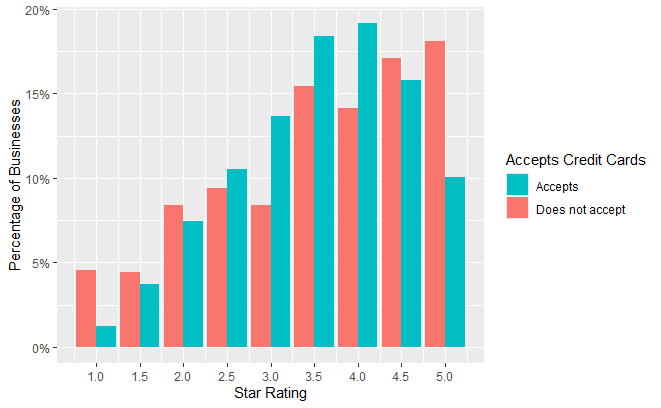
\includegraphics{figure1.png}

The weekly open-hour distribution indicated higher activity during
weekdays and reduced business activity on weekends, especially Sundays,
as visualized in the histogram.

\subsection{Spatial Analysis}\label{spatial-analysis}

Spatial autocorrelation analysis using variograms revealed increasing
semivariance with distance, supporting Tobler's first law, which states
that closer observations tend to be more similar than distant ones.

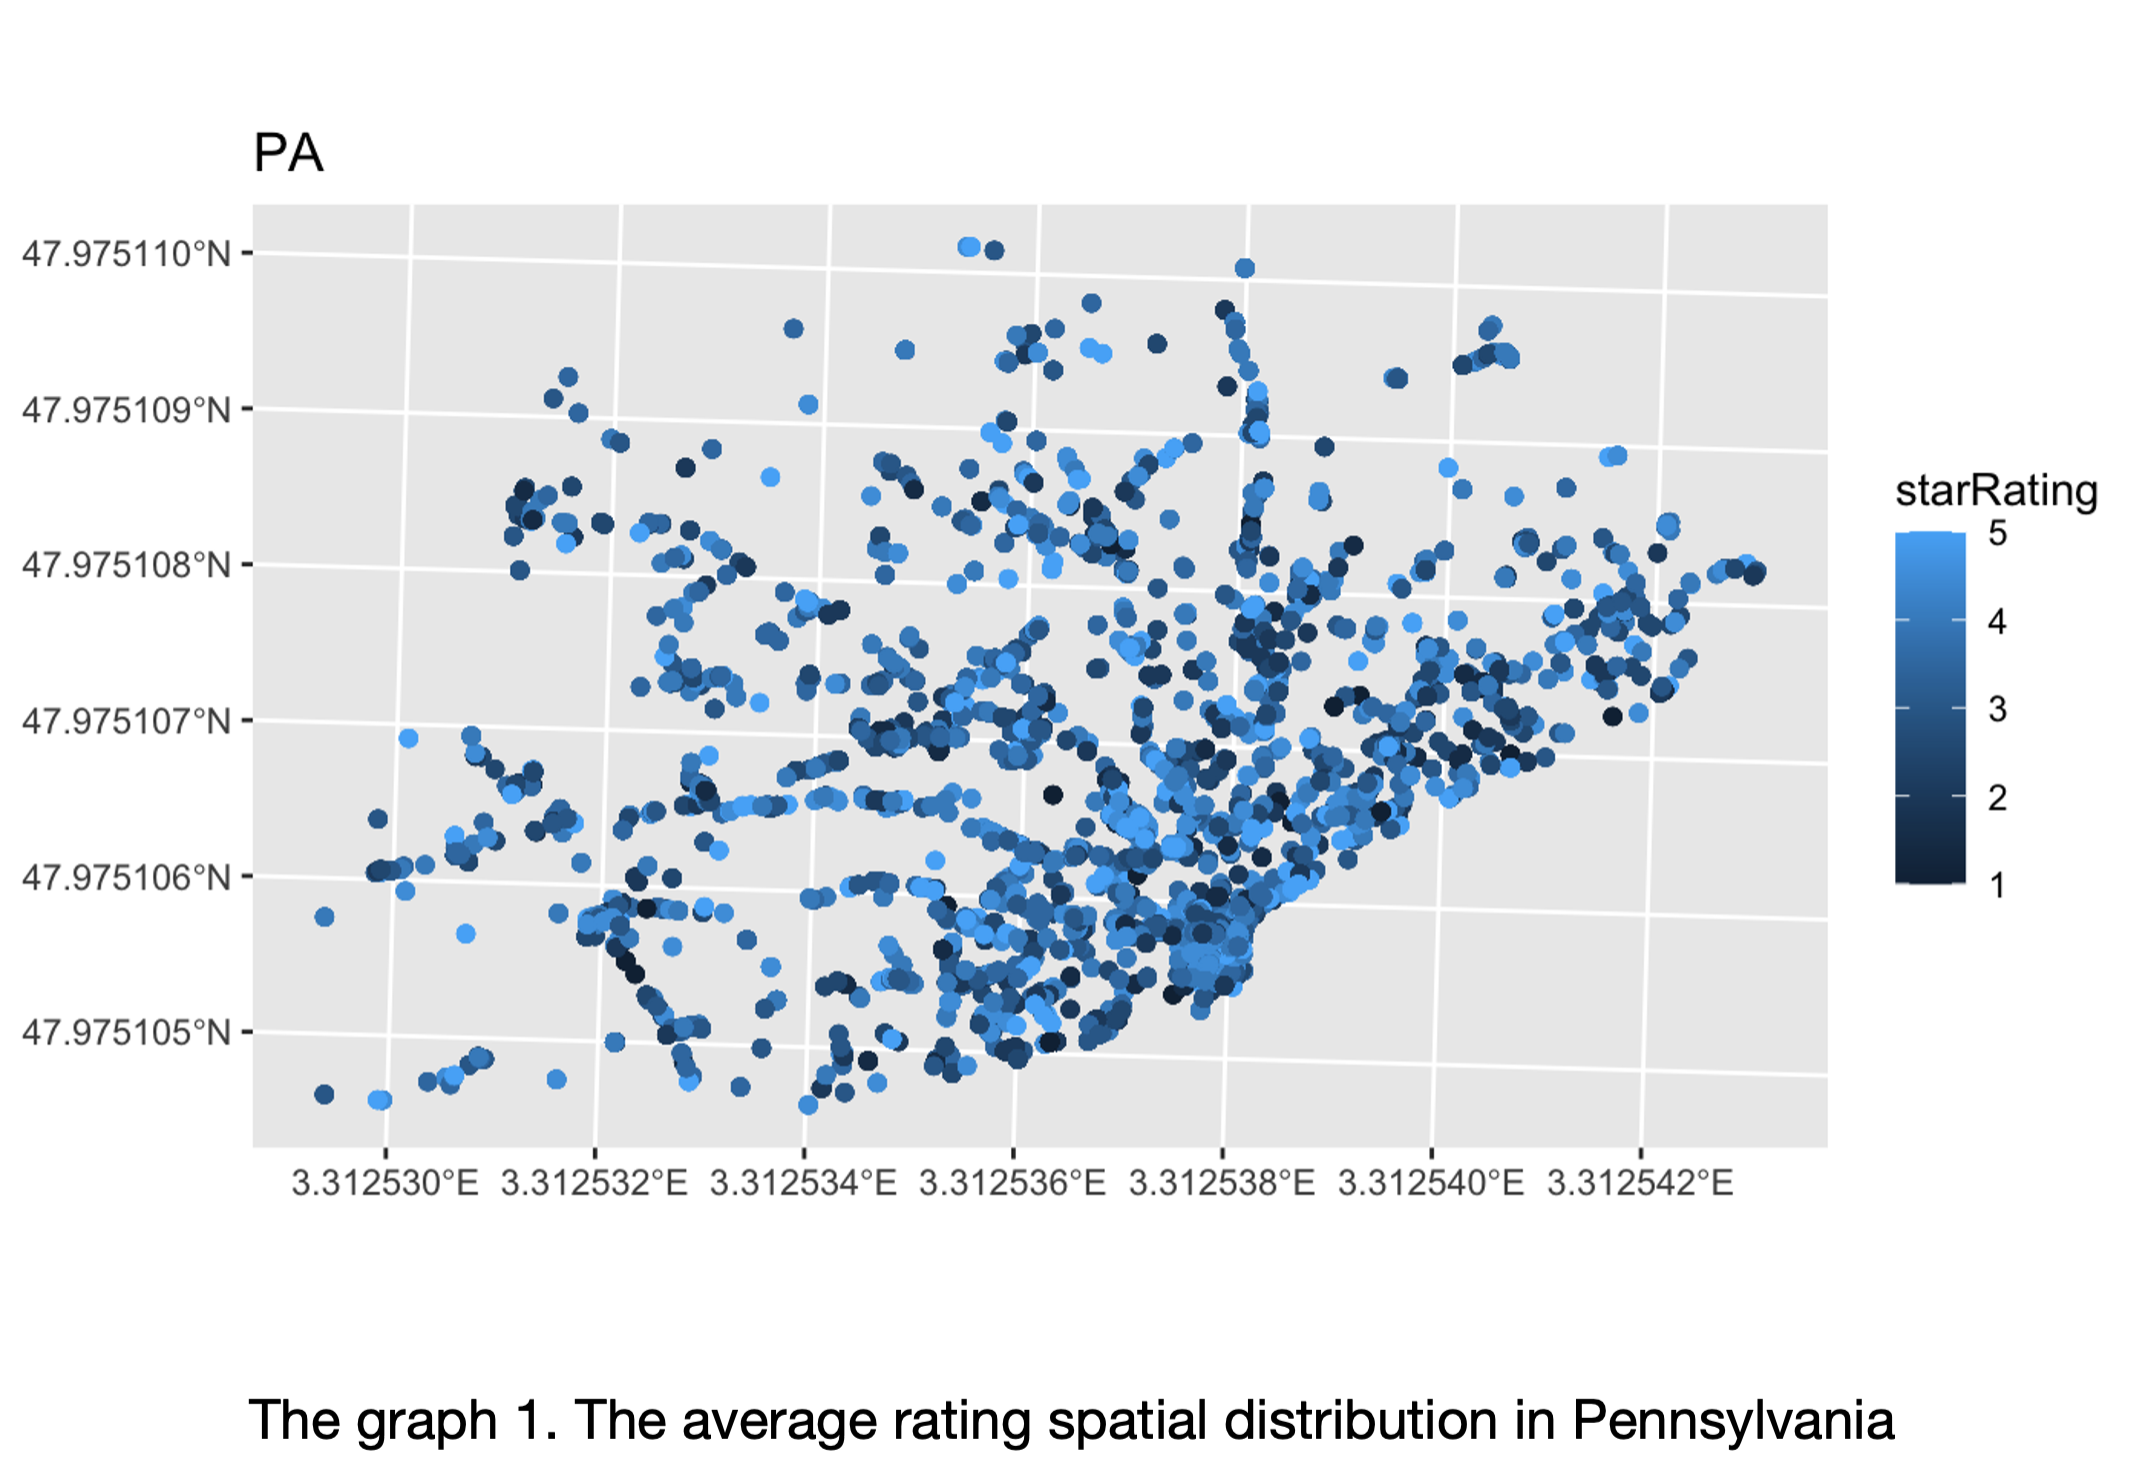
\includegraphics{figure2.png}

We fitted spatial linear models (\texttt{splm}) using the Matern
covariance function, identifying significant explanatory variables
influencing star ratings.

Spatial autocorrelation was confirmed, as ratings were more similar
among closer locations. The fitted variogram models aligned with
theoretical expectations, showing increasing semivariance with distance.

Specifically:

\begin{itemize}
\tightlist
\item
  \textbf{Credit card acceptance} significantly impacted star ratings in
  multiple states, notably IL, CA, IN, NJ, and DE.
\item
  \textbf{Review counts} (popularity indicator) also significantly
  influenced ratings in several states, underscoring the relationship
  between popularity and consumer satisfaction.
\item
  \textbf{Weekend operations} had a noticeable effect, particularly for
  businesses open on weekends, impacting ratings in select states.
\end{itemize}

\section{Conclusion}\label{conclusion}

Our analysis demonstrates that consumer star ratings exhibit notable
spatial correlation. Variables such as acceptance of credit cards,
review counts, and weekend operations significantly affect ratings and
differ regionally. Future analyses could include additional business
attributes or expand to broader geographical regions to provide deeper
insights.

\newpage{}

\section{Appendix}\label{appendix}

\subsection{Shiny Application}\label{shiny-application}

\textbf{Author:} Brian Cervantes Alvarez

\href{https://bcervantesalvarez.shinyapps.io/YelpReviewsDashboard/}{Shiny
Application}

\begin{Shaded}
\begin{Highlighting}[]
\CommentTok{\# app.R}

\FunctionTok{library}\NormalTok{(shiny)}
\FunctionTok{library}\NormalTok{(shinyjs)}
\FunctionTok{library}\NormalTok{(dplyr)}
\FunctionTok{library}\NormalTok{(readr)}
\FunctionTok{library}\NormalTok{(stringr)}
\FunctionTok{library}\NormalTok{(sf)}
\FunctionTok{library}\NormalTok{(leaflet)}
\FunctionTok{library}\NormalTok{(plotly)}
\FunctionTok{library}\NormalTok{(tidyr)}
\FunctionTok{library}\NormalTok{(lubridate)}
\FunctionTok{library}\NormalTok{(spmodel)}
\FunctionTok{library}\NormalTok{(gstat)}

\CommentTok{\#{-}{-}{-}{-}{-}{-}{-}{-}{-}{-}{-}{-}{-}{-}{-}{-}{-}{-}{-}{-}{-}{-}{-}{-}{-}{-}{-}{-}{-}}
\CommentTok{\# 1) Load Final Data}
\CommentTok{\#{-}{-}{-}{-}{-}{-}{-}{-}{-}{-}{-}{-}{-}{-}{-}{-}{-}{-}{-}{-}{-}{-}{-}{-}{-}{-}{-}{-}{-}}
\NormalTok{yelpDs }\OtherTok{\textless{}{-}} \FunctionTok{read\_csv}\NormalTok{(}\StringTok{"finalYelpData\_sampled.csv"}\NormalTok{) }\SpecialCharTok{\%\textgreater{}\%}
  \FunctionTok{filter}\NormalTok{(}\SpecialCharTok{!}\FunctionTok{is.na}\NormalTok{(latitude), }\SpecialCharTok{!}\FunctionTok{is.na}\NormalTok{(longitude))}

\CommentTok{\#{-}{-}{-}{-}{-}{-}{-}{-}{-}{-}{-}{-}{-}{-}{-}{-}{-}{-}{-}{-}{-}{-}{-}{-}{-}{-}{-}{-}{-}}
\CommentTok{\# 2) Helper Functions}
\CommentTok{\#{-}{-}{-}{-}{-}{-}{-}{-}{-}{-}{-}{-}{-}{-}{-}{-}{-}{-}{-}{-}{-}{-}{-}{-}{-}{-}{-}{-}{-}}
\NormalTok{convert\_hours\_str }\OtherTok{\textless{}{-}} \ControlFlowTok{function}\NormalTok{(h) \{}
  \ControlFlowTok{if}\NormalTok{ (}\FunctionTok{is.na}\NormalTok{(h) }\SpecialCharTok{||}\NormalTok{ h }\SpecialCharTok{==} \StringTok{"Closed"} \SpecialCharTok{||}\NormalTok{ h }\SpecialCharTok{==} \StringTok{"00:00:00 {-} 00:00:00"}\NormalTok{) \{}
    \FunctionTok{return}\NormalTok{(}\StringTok{"Closed"}\NormalTok{)}
\NormalTok{  \}}
\NormalTok{  parts }\OtherTok{\textless{}{-}} \FunctionTok{strsplit}\NormalTok{(h, }\StringTok{" {-} "}\NormalTok{)[[}\DecValTok{1}\NormalTok{]]}
  \ControlFlowTok{if}\NormalTok{ (}\FunctionTok{length}\NormalTok{(parts) }\SpecialCharTok{!=} \DecValTok{2}\NormalTok{) }\FunctionTok{return}\NormalTok{(}\StringTok{"Closed"}\NormalTok{)}
  
\NormalTok{  start\_time }\OtherTok{\textless{}{-}} \FunctionTok{strptime}\NormalTok{(parts[}\DecValTok{1}\NormalTok{], }\StringTok{"\%H:\%M:\%S"}\NormalTok{)}
\NormalTok{  end\_time   }\OtherTok{\textless{}{-}} \FunctionTok{strptime}\NormalTok{(parts[}\DecValTok{2}\NormalTok{], }\StringTok{"\%H:\%M:\%S"}\NormalTok{)}
  
\NormalTok{  start\_str }\OtherTok{\textless{}{-}} \FunctionTok{format}\NormalTok{(start\_time, }\StringTok{"\%I:\%M\%p"}\NormalTok{)}
\NormalTok{  end\_str   }\OtherTok{\textless{}{-}} \FunctionTok{format}\NormalTok{(end\_time,   }\StringTok{"\%I:\%M\%p"}\NormalTok{)}
  
  \CommentTok{\# Remove leading zero from hour}
\NormalTok{  start\_str }\OtherTok{\textless{}{-}} \FunctionTok{sub}\NormalTok{(}\StringTok{"\^{}0"}\NormalTok{, }\StringTok{""}\NormalTok{, start\_str)}
\NormalTok{  end\_str   }\OtherTok{\textless{}{-}} \FunctionTok{sub}\NormalTok{(}\StringTok{"\^{}0"}\NormalTok{, }\StringTok{""}\NormalTok{, end\_str)}
  
  \FunctionTok{paste}\NormalTok{(start\_str, }\StringTok{"{-}"}\NormalTok{, end\_str)}
\NormalTok{\}}

\NormalTok{star\_emoji }\OtherTok{\textless{}{-}} \FunctionTok{Vectorize}\NormalTok{(}\ControlFlowTok{function}\NormalTok{(rating) \{}
  \ControlFlowTok{if}\NormalTok{ (}\FunctionTok{is.na}\NormalTok{(rating) }\SpecialCharTok{||}\NormalTok{ rating }\SpecialCharTok{\textless{}=} \DecValTok{0}\NormalTok{) }\FunctionTok{return}\NormalTok{(}\StringTok{"No rating"}\NormalTok{)}
\NormalTok{  rating\_rounded\_half }\OtherTok{\textless{}{-}} \FunctionTok{round}\NormalTok{(rating }\SpecialCharTok{*} \DecValTok{2}\NormalTok{) }\SpecialCharTok{/} \DecValTok{2}
  \ControlFlowTok{if}\NormalTok{ (rating\_rounded\_half }\SpecialCharTok{\textgreater{}} \DecValTok{5}\NormalTok{) rating\_rounded\_half }\OtherTok{\textless{}{-}} \DecValTok{5}
\NormalTok{  full\_stars }\OtherTok{\textless{}{-}} \FunctionTok{floor}\NormalTok{(rating\_rounded\_half)}
\NormalTok{  half\_star  }\OtherTok{\textless{}{-}}\NormalTok{ (rating\_rounded\_half }\SpecialCharTok{{-}}\NormalTok{ full\_stars) }\SpecialCharTok{\textgreater{}=} \FloatTok{0.5}
\NormalTok{  star\_str   }\OtherTok{\textless{}{-}} \FunctionTok{paste}\NormalTok{(}\FunctionTok{rep}\NormalTok{(}\StringTok{"⭐"}\NormalTok{, full\_stars), }\AttributeTok{collapse=}\StringTok{""}\NormalTok{)}
  \ControlFlowTok{if}\NormalTok{ (half\_star) star\_str }\OtherTok{\textless{}{-}} \FunctionTok{paste0}\NormalTok{(star\_str, }\StringTok{"✨"}\NormalTok{)}
  \FunctionTok{paste0}\NormalTok{(rating, }\StringTok{" ("}\NormalTok{, star\_str, }\StringTok{")"}\NormalTok{)}
\NormalTok{\})}

\NormalTok{modelMap }\OtherTok{\textless{}{-}} \FunctionTok{c}\NormalTok{(}\AttributeTok{Sph=}\StringTok{"Spherical"}\NormalTok{, }\AttributeTok{Exp=}\StringTok{"Exponential"}\NormalTok{, }\AttributeTok{Mat=}\StringTok{"Matern"}\NormalTok{, }\AttributeTok{Gau=}\StringTok{"Gaussian"}\NormalTok{)}

\CommentTok{\#{-}{-}{-}{-}{-}{-}{-}{-}{-}{-}{-}{-}{-}{-}{-}{-}{-}{-}{-}{-}{-}{-}{-}{-}{-}{-}{-}{-}{-}}
\CommentTok{\# 3) USER INTERFACE (UI)}
\CommentTok{\#{-}{-}{-}{-}{-}{-}{-}{-}{-}{-}{-}{-}{-}{-}{-}{-}{-}{-}{-}{-}{-}{-}{-}{-}{-}{-}{-}{-}{-}}
\NormalTok{ui }\OtherTok{\textless{}{-}} \FunctionTok{withMathJax}\NormalTok{(}\FunctionTok{fluidPage}\NormalTok{(}
  \FunctionTok{useShinyjs}\NormalTok{(),}
\NormalTok{  tags}\SpecialCharTok{$}\FunctionTok{head}\NormalTok{(}
\NormalTok{    tags}\SpecialCharTok{$}\FunctionTok{link}\NormalTok{(}
      \AttributeTok{href=}\StringTok{"https://fonts.googleapis.com/css2?family=Open+Sans:wght@300;400;600\&display=swap"}\NormalTok{,}
      \AttributeTok{rel=}\StringTok{"stylesheet"}
\NormalTok{    ),}
    \CommentTok{\# Updated slider CSS: transparent unselected track, black active bar, orange handles}
\NormalTok{    tags}\SpecialCharTok{$}\FunctionTok{style}\NormalTok{(}\FunctionTok{HTML}\NormalTok{(}\StringTok{"}
\StringTok{      body \{}
\StringTok{        font{-}family: \textquotesingle{}Open Sans\textquotesingle{}, sans{-}serif;}
\StringTok{        background{-}color: \#FFFFFF;}
\StringTok{        color: \#000000;}
\StringTok{        font{-}size: 2rem;}
\StringTok{      \}}
\StringTok{      /* Tabset theme */}
\StringTok{      .nav{-}tabs\textgreater{}li\textgreater{}a \{}
\StringTok{        color: \#000000 !important; /* unselected tabs: black text */}
\StringTok{      \}}
\StringTok{      .nav{-}tabs\textgreater{}li\textgreater{}a:hover \{}
\StringTok{        background{-}color: \#D73F09 !important;}
\StringTok{        color: \#FFFFFF !important;}
\StringTok{        border{-}radius: 8px 8px 0 0;}
\StringTok{      \}}
\StringTok{      .nav{-}tabs\textgreater{}li.active\textgreater{}a,}
\StringTok{      .nav{-}tabs\textgreater{}li.active\textgreater{}a:focus,}
\StringTok{      .nav{-}tabs\textgreater{}li.active\textgreater{}a:hover \{}
\StringTok{        background{-}color: \#D73F09 !important;}
\StringTok{        color: \#FFFFFF !important;}
\StringTok{        border{-}radius: 8px 8px 0 0;}
\StringTok{      \}}

\StringTok{      /* Slider theme:}
\StringTok{         {-} transparent unselected track}
\StringTok{         {-} black active bar}
\StringTok{         {-} orange handles (\#D73F09)}
\StringTok{      */}
\StringTok{      .js{-}range{-}slider .irs{-}line \{}
\StringTok{        background: transparent !important;}
\StringTok{        border: none !important;}
\StringTok{      \}}
\StringTok{      .js{-}range{-}slider .irs{-}bar,}
\StringTok{      .js{-}range{-}slider .irs{-}bar{-}edge \{}
\StringTok{        background: \#000000 !important; /* black active region */}
\StringTok{        border{-}color: \#000000 !important;}
\StringTok{      \}}
\StringTok{      .js{-}range{-}slider .irs{-}handle\textgreater{}i,}
\StringTok{      .js{-}range{-}slider .irs{-}handle\textgreater{}i:first{-}child,}
\StringTok{      .js{-}range{-}slider .irs{-}handle\textgreater{}i:last{-}child \{}
\StringTok{        background: \#D73F09 !important; /* orange handles */}
\StringTok{        border{-}color: \#D73F09 !important;}
\StringTok{      \}}
\StringTok{      .js{-}range{-}slider .irs{-}single,}
\StringTok{      .js{-}range{-}slider .irs{-}to,}
\StringTok{      .js{-}range{-}slider .irs{-}from \{}
\StringTok{        background: \#000000 !important;}
\StringTok{        border{-}color: \#000000 !important;}
\StringTok{        color: \#FFFFFF !important;}
\StringTok{      \}}

\StringTok{      /* Box shadow class */}
\StringTok{      .boxShadow \{}
\StringTok{        box{-}shadow: rgba(0,0,0,0.25) 0px 54px 55px,}
\StringTok{                    rgba(0,0,0,0.12) 0px {-}12px 30px,}
\StringTok{                    rgba(0,0,0,0.12) 0px 4px 6px,}
\StringTok{                    rgba(0,0,0,0.17) 0px 12px 13px,}
\StringTok{                    rgba(0,0,0,0.09) 0px {-}3px 5px;}
\StringTok{        border{-}radius: 15px;}
\StringTok{      \}}
\StringTok{      \#reviewMap \{}
\StringTok{        width: 100\% !important;}
\StringTok{        height: 75vh !important;}
\StringTok{      \}}
\StringTok{      /* Top banner */}
\StringTok{      \#topBanner \{}
\StringTok{        background{-}color: \#D73F09;}
\StringTok{        color: \#FFFFFF;}
\StringTok{        padding: 15px;}
\StringTok{        margin: 10px;}
\StringTok{        border{-}radius: 8px;}
\StringTok{      \}}
\StringTok{      \#yelpLogoContainer \{}
\StringTok{        text{-}align: right;}
\StringTok{      \}}
\StringTok{      \#yelpLogoContainer div \{}
\StringTok{        display: inline{-}block;}
\StringTok{        background{-}color: \#FFFFFF;}
\StringTok{        padding: 5px;}
\StringTok{        border{-}radius: 8px;}
\StringTok{      \}}
\StringTok{      \#yelpLogoContainer img \{}
\StringTok{        width: 60px;}
\StringTok{      \}}
\StringTok{      .marker{-}cluster div \{}
\StringTok{        background{-}color: rgba(0,0,0,0.7) !important;}
\StringTok{        border{-}radius: 20px;}
\StringTok{        width: 40px;}
\StringTok{        height: 40px;}
\StringTok{        line{-}height: 40px;}
\StringTok{        color: \#FFFFFF !important;}
\StringTok{        text{-}align: center;}
\StringTok{      \}}

\StringTok{      /* Provide some vertical spacing for sidebars */}
\StringTok{      \#map\_sidebar,}
\StringTok{      \#cc\_sidebar,}
\StringTok{      \#facet\_sidebar,}
\StringTok{      \#wh\_sidebar,}
\StringTok{      \#dist\_sidebar,}
\StringTok{      \#star\_sidebar \{}
\StringTok{        margin{-}top: 15px;}
\StringTok{      \}}
\StringTok{      .form{-}group \{}
\StringTok{        margin{-}bottom: 15px !important;}
\StringTok{      \}}

\StringTok{      /* Black background, white text for selectInput */}
\StringTok{      .selectize{-}control.single .selectize{-}input \{}
\StringTok{        background{-}color: \#000000 !important;}
\StringTok{        color: \#FFFFFF !important;}
\StringTok{        border: 1px solid \#000000 !important;}
\StringTok{      \}}
\StringTok{      .selectize{-}dropdown,}
\StringTok{      .selectize{-}dropdown{-}content,}
\StringTok{      .selectize{-}control.single .selectize{-}input.dropdown{-}active \{}
\StringTok{        background{-}color: \#000000 !important;}
\StringTok{        color: \#FFFFFF !important;}
\StringTok{        border: 1px solid \#000000 !important;}
\StringTok{      \}}
\StringTok{    "}\NormalTok{))}
\NormalTok{  ),}
  
  \FunctionTok{fluidRow}\NormalTok{(}
    \AttributeTok{id=}\StringTok{"topBanner"}\NormalTok{,}
    \FunctionTok{column}\NormalTok{(}
      \AttributeTok{width=}\DecValTok{9}\NormalTok{,}
\NormalTok{      tags}\SpecialCharTok{$}\FunctionTok{h2}\NormalTok{(}\StringTok{"Yelp Reviews on Businesses Dashboard"}\NormalTok{),}
\NormalTok{      tags}\SpecialCharTok{$}\FunctionTok{p}\NormalTok{(}\StringTok{"This Shiny application showcases real{-}world data related to businesses and includes actual customer reviews. Explore star ratings, open hours, and spatial analysis with variogram modeling."}\NormalTok{)}
\NormalTok{    ),}
    \FunctionTok{column}\NormalTok{(}
      \AttributeTok{width=}\DecValTok{3}\NormalTok{,}
      \FunctionTok{div}\NormalTok{(}
        \AttributeTok{id=}\StringTok{"yelpLogoContainer"}\NormalTok{,}
        \FunctionTok{div}\NormalTok{(}
          \FunctionTok{img}\NormalTok{(}\AttributeTok{src=}\StringTok{"https://raw.githubusercontent.com/bcervantesalvarez/Portfolio/refs/heads/main/Assets/Images/yelpBurst.svg"}\NormalTok{, }\AttributeTok{alt=}\StringTok{"Yelp Logo"}\NormalTok{)}
\NormalTok{        )}
\NormalTok{      )}
\NormalTok{    )}
\NormalTok{  ),}
  \FunctionTok{br}\NormalTok{(),}
  
  \FunctionTok{tabsetPanel}\NormalTok{(}
    \CommentTok{\#=========================}
    \CommentTok{\# TAB 1: SPATIAL MAP}
    \CommentTok{\#=========================}
    \FunctionTok{tabPanel}\NormalTok{(}\StringTok{"Spatial Map"}\NormalTok{,}
      \FunctionTok{fluidRow}\NormalTok{(}
        \FunctionTok{column}\NormalTok{(}
          \AttributeTok{width=}\DecValTok{3}\NormalTok{,}
          \AttributeTok{id=}\StringTok{"map\_sidebar"}\NormalTok{,}
          \FunctionTok{selectInput}\NormalTok{(}\StringTok{"citySelect"}\NormalTok{, }\StringTok{"City:"}\NormalTok{, }\AttributeTok{choices=}\FunctionTok{c}\NormalTok{(}\StringTok{"All"}\NormalTok{, }\FunctionTok{sort}\NormalTok{(}\FunctionTok{unique}\NormalTok{(yelpDs}\SpecialCharTok{$}\NormalTok{city)))),}
          \FunctionTok{sliderInput}\NormalTok{(}\StringTok{"ratingRange"}\NormalTok{, }\StringTok{"Star Rating:"}\NormalTok{, }\AttributeTok{min=}\DecValTok{1}\NormalTok{, }\AttributeTok{max=}\DecValTok{5}\NormalTok{, }\AttributeTok{value=}\FunctionTok{c}\NormalTok{(}\DecValTok{1}\NormalTok{,}\DecValTok{5}\NormalTok{))}
\NormalTok{        ),}
        \FunctionTok{column}\NormalTok{(}
          \AttributeTok{width=}\DecValTok{9}\NormalTok{,}
          \AttributeTok{id=}\StringTok{"map\_main"}\NormalTok{,}
          \FunctionTok{actionButton}\NormalTok{(}\StringTok{"toggle\_map"}\NormalTok{, }\StringTok{"Hide Filters"}\NormalTok{),}
\NormalTok{          tags}\SpecialCharTok{$}\FunctionTok{h4}\NormalTok{(}\StringTok{"About the Spatial Map"}\NormalTok{),}
\NormalTok{          tags}\SpecialCharTok{$}\FunctionTok{p}\NormalTok{(}\StringTok{"This interactive map displays the locations of Yelp businesses based on your selected city and star rating range. Individual markers represent each business, and when many businesses are located close together, they group into clusters that you can click to zoom in and view more detail."}\NormalTok{),}
          \FunctionTok{div}\NormalTok{(}\AttributeTok{class=}\StringTok{"boxShadow"}\NormalTok{, }\FunctionTok{leafletOutput}\NormalTok{(}\StringTok{"reviewMap"}\NormalTok{, }\AttributeTok{height=}\StringTok{"600px"}\NormalTok{))}
\NormalTok{        )}
\NormalTok{      )}
\NormalTok{    ),}
    
    \CommentTok{\#=========================}
    \CommentTok{\# TAB 2: DATA VISUALIZATION}
    \CommentTok{\#=========================}
    \FunctionTok{tabPanel}\NormalTok{(}\StringTok{"Data Visualization"}\NormalTok{,}
      \FunctionTok{tabsetPanel}\NormalTok{(}
      \CommentTok{\# 2.1: Credit Cards vs. Star Rating}
      \FunctionTok{tabPanel}\NormalTok{(}\StringTok{"Credit Cards vs. Star Rating"}\NormalTok{,}
        \FunctionTok{fluidRow}\NormalTok{(}
          \FunctionTok{column}\NormalTok{(}
            \AttributeTok{width=}\DecValTok{3}\NormalTok{,}
            \AttributeTok{id=}\StringTok{"cc\_sidebar"}\NormalTok{,}
            \FunctionTok{selectInput}\NormalTok{(}\StringTok{"ccCity"}\NormalTok{, }\StringTok{"City:"}\NormalTok{, }\AttributeTok{choices=}\FunctionTok{c}\NormalTok{(}\StringTok{"All"}\NormalTok{, }\FunctionTok{sort}\NormalTok{(}\FunctionTok{unique}\NormalTok{(yelpDs}\SpecialCharTok{$}\NormalTok{city)))),}
            \FunctionTok{sliderInput}\NormalTok{(}\StringTok{"ccStarRange"}\NormalTok{, }\StringTok{"Star Rating:"}\NormalTok{, }\AttributeTok{min=}\DecValTok{1}\NormalTok{, }\AttributeTok{max=}\DecValTok{5}\NormalTok{, }\AttributeTok{value=}\FunctionTok{c}\NormalTok{(}\DecValTok{1}\NormalTok{,}\DecValTok{5}\NormalTok{))}
\NormalTok{          ),}
          \FunctionTok{column}\NormalTok{(}
            \AttributeTok{width=}\DecValTok{9}\NormalTok{,}
            \AttributeTok{id=}\StringTok{"cc\_main"}\NormalTok{,}
            \FunctionTok{actionButton}\NormalTok{(}\StringTok{"toggle\_cc"}\NormalTok{, }\StringTok{"Hide Filters"}\NormalTok{),}
\NormalTok{            tags}\SpecialCharTok{$}\FunctionTok{h4}\NormalTok{(}\StringTok{"Credit Cards vs. Star Rating"}\NormalTok{),}
\NormalTok{            tags}\SpecialCharTok{$}\FunctionTok{p}\NormalTok{(}\StringTok{"This plot shows the proportion of businesses accepting credit cards across different star ratings. Filter by city and star rating range to narrow the results."}\NormalTok{),}
            \FunctionTok{div}\NormalTok{(}\AttributeTok{class=}\StringTok{"boxShadow"}\NormalTok{, }\FunctionTok{plotlyOutput}\NormalTok{(}\StringTok{"creditCardStarPlot"}\NormalTok{, }\AttributeTok{height=}\StringTok{"600px"}\NormalTok{))}
\NormalTok{          )}
\NormalTok{        )}
\NormalTok{        ),}
      \CommentTok{\# 2.2: Open Hours by Day}
      \FunctionTok{tabPanel}\NormalTok{(}\StringTok{"Open Hours by Day"}\NormalTok{,}
        \FunctionTok{fluidRow}\NormalTok{(}
          \FunctionTok{column}\NormalTok{(}
            \AttributeTok{width=}\DecValTok{3}\NormalTok{,}
            \AttributeTok{id=}\StringTok{"facet\_sidebar"}\NormalTok{,}
            \FunctionTok{selectInput}\NormalTok{(}\StringTok{"facetCity"}\NormalTok{, }\StringTok{"City:"}\NormalTok{, }\AttributeTok{choices=}\FunctionTok{c}\NormalTok{(}\StringTok{"All"}\NormalTok{, }\FunctionTok{sort}\NormalTok{(}\FunctionTok{unique}\NormalTok{(yelpDs}\SpecialCharTok{$}\NormalTok{city)))),}
            \FunctionTok{sliderInput}\NormalTok{(}\StringTok{"facetStarRange"}\NormalTok{, }\StringTok{"Star Rating:"}\NormalTok{, }\AttributeTok{min=}\DecValTok{1}\NormalTok{, }\AttributeTok{max=}\DecValTok{5}\NormalTok{, }\AttributeTok{value=}\FunctionTok{c}\NormalTok{(}\DecValTok{1}\NormalTok{,}\DecValTok{5}\NormalTok{)),}
            \FunctionTok{checkboxGroupInput}\NormalTok{(}\StringTok{"whichDays"}\NormalTok{, }\StringTok{"Days of Week to Show:"}\NormalTok{,}
              \AttributeTok{choices=}\FunctionTok{c}\NormalTok{(}\StringTok{"Monday"}\OtherTok{=}\StringTok{"monday\_open\_hours"}\NormalTok{,}
                        \StringTok{"Tuesday"}\OtherTok{=}\StringTok{"tuesday\_open\_hours"}\NormalTok{,}
                        \StringTok{"Wednesday"}\OtherTok{=}\StringTok{"wednesday\_open\_hours"}\NormalTok{,}
                        \StringTok{"Thursday"}\OtherTok{=}\StringTok{"thursday\_open\_hours"}\NormalTok{,}
                        \StringTok{"Friday"}\OtherTok{=}\StringTok{"friday\_open\_hours"}\NormalTok{,}
                        \StringTok{"Saturday"}\OtherTok{=}\StringTok{"saturday\_open\_hours"}\NormalTok{,}
                        \StringTok{"Sunday"}\OtherTok{=}\StringTok{"sunday\_open\_hours"}\NormalTok{),}
              \AttributeTok{selected=}\FunctionTok{c}\NormalTok{(}\StringTok{"monday\_open\_hours"}\NormalTok{,}
                        \StringTok{"tuesday\_open\_hours"}\NormalTok{,}
                        \StringTok{"wednesday\_open\_hours"}\NormalTok{,}
                        \StringTok{"thursday\_open\_hours"}\NormalTok{,}
                        \StringTok{"friday\_open\_hours"}\NormalTok{,}
                        \StringTok{"saturday\_open\_hours"}\NormalTok{,}
                        \StringTok{"sunday\_open\_hours"}\NormalTok{)}
\NormalTok{            )}
\NormalTok{          ),}
          \FunctionTok{column}\NormalTok{(}
            \AttributeTok{width=}\DecValTok{9}\NormalTok{,}
            \AttributeTok{id=}\StringTok{"facet\_main"}\NormalTok{,}
            \FunctionTok{actionButton}\NormalTok{(}\StringTok{"toggle\_facet"}\NormalTok{, }\StringTok{"Hide Filters"}\NormalTok{),}
\NormalTok{            tags}\SpecialCharTok{$}\FunctionTok{h4}\NormalTok{(}\StringTok{"Open Hours by Day"}\NormalTok{),}
\NormalTok{            tags}\SpecialCharTok{$}\FunctionTok{p}\NormalTok{(}\StringTok{"Examine how businesses\textquotesingle{} daily open hours are distributed. Select which days to display, and filter by city and star rating."}\NormalTok{),}
            \FunctionTok{div}\NormalTok{(}\AttributeTok{class=}\StringTok{"boxShadow"}\NormalTok{, }\FunctionTok{plotlyOutput}\NormalTok{(}\StringTok{"openHoursDistribution"}\NormalTok{, }\AttributeTok{height=}\StringTok{"600px"}\NormalTok{))}
\NormalTok{          )}
\NormalTok{        )}
\NormalTok{        ),}
      \CommentTok{\# 2.3: Weekly Hours vs. Star Rating}
      \FunctionTok{tabPanel}\NormalTok{(}\StringTok{"Weekly Hours vs. Star Rating"}\NormalTok{,}
        \FunctionTok{fluidRow}\NormalTok{(}
          \FunctionTok{column}\NormalTok{(}
            \AttributeTok{width=}\DecValTok{3}\NormalTok{,}
            \AttributeTok{id=}\StringTok{"wh\_sidebar"}\NormalTok{,}
            \FunctionTok{selectInput}\NormalTok{(}\StringTok{"whCity"}\NormalTok{, }\StringTok{"City:"}\NormalTok{, }\AttributeTok{choices=}\FunctionTok{c}\NormalTok{(}\StringTok{"All"}\NormalTok{, }\FunctionTok{sort}\NormalTok{(}\FunctionTok{unique}\NormalTok{(yelpDs}\SpecialCharTok{$}\NormalTok{city)))),}
            \FunctionTok{sliderInput}\NormalTok{(}\StringTok{"whStarRange"}\NormalTok{, }\StringTok{"Star Rating:"}\NormalTok{, }\AttributeTok{min=}\DecValTok{1}\NormalTok{, }\AttributeTok{max=}\DecValTok{5}\NormalTok{, }\AttributeTok{value=}\FunctionTok{c}\NormalTok{(}\DecValTok{1}\NormalTok{,}\DecValTok{5}\NormalTok{)),}
            \FunctionTok{sliderInput}\NormalTok{(}\StringTok{"whHourRange"}\NormalTok{, }\StringTok{"Weekly Hours Range:"}\NormalTok{, }\AttributeTok{min=}\DecValTok{0}\NormalTok{, }\AttributeTok{max=}\DecValTok{168}\NormalTok{, }\AttributeTok{value=}\FunctionTok{c}\NormalTok{(}\DecValTok{0}\NormalTok{,}\DecValTok{168}\NormalTok{))}
\NormalTok{          ),}
          \FunctionTok{column}\NormalTok{(}
            \AttributeTok{width=}\DecValTok{9}\NormalTok{,}
            \AttributeTok{id=}\StringTok{"wh\_main"}\NormalTok{,}
            \FunctionTok{actionButton}\NormalTok{(}\StringTok{"toggle\_wh"}\NormalTok{, }\StringTok{"Hide Filters"}\NormalTok{),}
\NormalTok{            tags}\SpecialCharTok{$}\FunctionTok{h4}\NormalTok{(}\StringTok{"Weekly Hours vs. Star Rating"}\NormalTok{),}
\NormalTok{            tags}\SpecialCharTok{$}\FunctionTok{p}\NormalTok{(}\StringTok{"This bar chart shows average weekly open hours grouped by star rating. Adjust city, rating range, and weekly hours range to explore relationships."}\NormalTok{),}
            \FunctionTok{div}\NormalTok{(}\AttributeTok{class=}\StringTok{"boxShadow"}\NormalTok{, }\FunctionTok{plotlyOutput}\NormalTok{(}\StringTok{"openHoursVsStar"}\NormalTok{, }\AttributeTok{height=}\StringTok{"600px"}\NormalTok{))}
\NormalTok{          )}
\NormalTok{        )}
\NormalTok{        ),}
      \CommentTok{\# 2.4: Distribution of Weekly Hours}
      \FunctionTok{tabPanel}\NormalTok{(}\StringTok{"Distribution of Weekly Hours"}\NormalTok{,}
        \FunctionTok{fluidRow}\NormalTok{(}
          \FunctionTok{column}\NormalTok{(}
            \AttributeTok{width=}\DecValTok{3}\NormalTok{,}
            \AttributeTok{id=}\StringTok{"dist\_sidebar"}\NormalTok{,}
            \FunctionTok{selectInput}\NormalTok{(}\StringTok{"distCity"}\NormalTok{, }\StringTok{"City:"}\NormalTok{, }\AttributeTok{choices=}\FunctionTok{c}\NormalTok{(}\StringTok{"All"}\NormalTok{, }\FunctionTok{sort}\NormalTok{(}\FunctionTok{unique}\NormalTok{(yelpDs}\SpecialCharTok{$}\NormalTok{city)))),}
            \FunctionTok{sliderInput}\NormalTok{(}\StringTok{"distHourRange"}\NormalTok{, }\StringTok{"Weekly Hours Range:"}\NormalTok{, }\AttributeTok{min=}\DecValTok{0}\NormalTok{, }\AttributeTok{max=}\DecValTok{168}\NormalTok{, }\AttributeTok{value=}\FunctionTok{c}\NormalTok{(}\DecValTok{0}\NormalTok{,}\DecValTok{168}\NormalTok{))}
\NormalTok{          ),}
          \FunctionTok{column}\NormalTok{(}
            \AttributeTok{width=}\DecValTok{9}\NormalTok{,}
            \AttributeTok{id=}\StringTok{"dist\_main"}\NormalTok{,}
            \FunctionTok{actionButton}\NormalTok{(}\StringTok{"toggle\_dist"}\NormalTok{, }\StringTok{"Hide Filters"}\NormalTok{),}
\NormalTok{            tags}\SpecialCharTok{$}\FunctionTok{h4}\NormalTok{(}\StringTok{"Distribution of Weekly Hours"}\NormalTok{),}
\NormalTok{            tags}\SpecialCharTok{$}\FunctionTok{p}\NormalTok{(}\StringTok{"This histogram shows how many businesses fall into various weekly open{-}hour bins. Filter by city or choose a smaller hour range to focus on specific subsets."}\NormalTok{),}
            \FunctionTok{div}\NormalTok{(}\AttributeTok{class=}\StringTok{"boxShadow"}\NormalTok{, }\FunctionTok{plotlyOutput}\NormalTok{(}\StringTok{"weeklyHoursPlot"}\NormalTok{, }\AttributeTok{height=}\StringTok{"600px"}\NormalTok{))}
\NormalTok{          )}
\NormalTok{        )}
\NormalTok{        ),}
      \CommentTok{\# 2.5: Distribution of Star Ratings}
      \FunctionTok{tabPanel}\NormalTok{(}\StringTok{"Distribution of Star Ratings"}\NormalTok{,}
        \FunctionTok{fluidRow}\NormalTok{(}
          \FunctionTok{column}\NormalTok{(}
            \AttributeTok{width=}\DecValTok{3}\NormalTok{,}
            \AttributeTok{id=}\StringTok{"star\_sidebar"}\NormalTok{,}
            \FunctionTok{selectInput}\NormalTok{(}\StringTok{"starCity"}\NormalTok{, }\StringTok{"City:"}\NormalTok{, }\AttributeTok{choices=}\FunctionTok{c}\NormalTok{(}\StringTok{"All"}\NormalTok{, }\FunctionTok{sort}\NormalTok{(}\FunctionTok{unique}\NormalTok{(yelpDs}\SpecialCharTok{$}\NormalTok{city)))),}
            \FunctionTok{sliderInput}\NormalTok{(}\StringTok{"starFilterRange"}\NormalTok{, }\StringTok{"Star Rating Range:"}\NormalTok{, }\AttributeTok{min=}\DecValTok{1}\NormalTok{, }\AttributeTok{max=}\DecValTok{5}\NormalTok{, }\AttributeTok{value=}\FunctionTok{c}\NormalTok{(}\DecValTok{1}\NormalTok{,}\DecValTok{5}\NormalTok{))}
\NormalTok{          ),}
          \FunctionTok{column}\NormalTok{(}
            \AttributeTok{width=}\DecValTok{9}\NormalTok{,}
            \AttributeTok{id=}\StringTok{"star\_main"}\NormalTok{,}
            \FunctionTok{actionButton}\NormalTok{(}\StringTok{"toggle\_star"}\NormalTok{, }\StringTok{"Hide Filters"}\NormalTok{),}
\NormalTok{            tags}\SpecialCharTok{$}\FunctionTok{h4}\NormalTok{(}\StringTok{"Distribution of Star Ratings"}\NormalTok{),}
\NormalTok{            tags}\SpecialCharTok{$}\FunctionTok{p}\NormalTok{(}\StringTok{"View how star ratings are distributed among businesses. Filter by city or rating range to examine particular subsets."}\NormalTok{),}
            \FunctionTok{div}\NormalTok{(}\AttributeTok{class=}\StringTok{"boxShadow"}\NormalTok{, }\FunctionTok{plotlyOutput}\NormalTok{(}\StringTok{"distStarRatingPlot"}\NormalTok{, }\AttributeTok{height=}\StringTok{"600px"}\NormalTok{))}
\NormalTok{          )}
\NormalTok{        )}
\NormalTok{        )}
\NormalTok{      )}
\NormalTok{    ),}
    
    \CommentTok{\#=========================}
    \CommentTok{\# TAB 3: SPATIAL MODELING}
    \CommentTok{\#=========================}
    \FunctionTok{tabPanel}\NormalTok{(}\StringTok{"Spatial Modeling"}\NormalTok{,}
      \FunctionTok{sidebarLayout}\NormalTok{(}
        \FunctionTok{sidebarPanel}\NormalTok{(}
\NormalTok{          tags}\SpecialCharTok{$}\FunctionTok{div}\NormalTok{(}
            \AttributeTok{style=}\StringTok{"border:1px solid \#ccc; background{-}color:\#ffffcc; padding:8px; margin{-}bottom:10px;"}\NormalTok{,}
            \StringTok{"Warning: This model can take 15 seconds to 10 minutes depending on the State that is chosen."}
\NormalTok{          ),}
          \FunctionTok{selectInput}\NormalTok{(}\StringTok{"stateChoice"}\NormalTok{, }\StringTok{"Choose a State:"}\NormalTok{,}
                      \AttributeTok{choices=}\FunctionTok{sort}\NormalTok{(}\FunctionTok{unique}\NormalTok{(yelpDs}\SpecialCharTok{$}\NormalTok{state)), }\AttributeTok{selected=}\StringTok{"NJ"}\NormalTok{),}
          \FunctionTok{selectInput}\NormalTok{(}\StringTok{"modelChoice"}\NormalTok{, }\StringTok{"Model Type:"}\NormalTok{,}
                      \AttributeTok{choices=}\FunctionTok{c}\NormalTok{(}\StringTok{"Variogram only"}\NormalTok{, }\StringTok{"Variogram + Fit"}\NormalTok{)),}
          \FunctionTok{selectInput}\NormalTok{(}\StringTok{"vgmType"}\NormalTok{, }\StringTok{"Variogram Model:"}\NormalTok{,}
                      \AttributeTok{choices=}\FunctionTok{c}\NormalTok{(}\StringTok{"Sph"}\NormalTok{, }\StringTok{"Exp"}\NormalTok{, }\StringTok{"Mat"}\NormalTok{, }\StringTok{"Gau"}\NormalTok{),}
                      \AttributeTok{selected=}\StringTok{"Sph"}\NormalTok{),}
          \FunctionTok{numericInput}\NormalTok{(}\StringTok{"psillInit"}\NormalTok{, }\StringTok{"Initial Partial Sill:"}\NormalTok{, }\AttributeTok{value=}\FloatTok{0.1}\NormalTok{, }\AttributeTok{min=}\DecValTok{0}\NormalTok{, }\AttributeTok{max=}\DecValTok{999}\NormalTok{, }\AttributeTok{step=}\FloatTok{0.01}\NormalTok{),}
          \FunctionTok{numericInput}\NormalTok{(}\StringTok{"rangeInit"}\NormalTok{, }\StringTok{"Initial Range:"}\NormalTok{, }\AttributeTok{value=}\FloatTok{0.5}\NormalTok{, }\AttributeTok{min=}\DecValTok{0}\NormalTok{, }\AttributeTok{max=}\DecValTok{999}\NormalTok{, }\AttributeTok{step=}\FloatTok{0.01}\NormalTok{),}
          \FunctionTok{numericInput}\NormalTok{(}\StringTok{"nuggetInit"}\NormalTok{, }\StringTok{"Initial Nugget:"}\NormalTok{, }\AttributeTok{value=}\FloatTok{0.01}\NormalTok{, }\AttributeTok{min=}\DecValTok{0}\NormalTok{, }\AttributeTok{max=}\DecValTok{999}\NormalTok{, }\AttributeTok{step=}\FloatTok{0.01}\NormalTok{),}
          \FunctionTok{numericInput}\NormalTok{(}\StringTok{"kappaInit"}\NormalTok{, }\StringTok{"Kappa (Matern only):"}\NormalTok{, }\AttributeTok{value=}\DecValTok{1}\NormalTok{, }\AttributeTok{min=}\FloatTok{0.01}\NormalTok{, }\AttributeTok{max=}\DecValTok{5}\NormalTok{, }\AttributeTok{step=}\FloatTok{0.01}\NormalTok{),}
          \FunctionTok{actionButton}\NormalTok{(}\StringTok{"runModel"}\NormalTok{, }\StringTok{"Run Model"}\NormalTok{)}
\NormalTok{        ),}
        \FunctionTok{mainPanel}\NormalTok{(}
          \FunctionTok{fluidRow}\NormalTok{(}
            \FunctionTok{column}\NormalTok{(}
              \AttributeTok{width=}\DecValTok{12}\NormalTok{,}
\NormalTok{              tags}\SpecialCharTok{$}\FunctionTok{h4}\NormalTok{(}\StringTok{"Spatial Modeling: Variogram Overview"}\NormalTok{),}
\NormalTok{              tags}\SpecialCharTok{$}\FunctionTok{p}\NormalTok{(}
                \StringTok{"A variogram measures how the differences in your data change with distance. We examine star ratings to see potential spatial clustering. One common formulation is "}\NormalTok{,}
                \FunctionTok{withMathJax}\NormalTok{(}\StringTok{"$$}\SpecialCharTok{\textbackslash{}\textbackslash{}}\StringTok{gamma(h) = }\SpecialCharTok{\textbackslash{}\textbackslash{}}\StringTok{frac\{1\}\{2N(h)\} }\SpecialCharTok{\textbackslash{}\textbackslash{}}\StringTok{sum\_\{i,j}\SpecialCharTok{\textbackslash{}\textbackslash{}}\StringTok{in h\} [z(x\_i){-}z(x\_j)]\^{}2,$$"}\NormalTok{),}
                \StringTok{" where }\SpecialCharTok{\textbackslash{}\textbackslash{}}\StringTok{(z(x\_i)}\SpecialCharTok{\textbackslash{}\textbackslash{}}\StringTok{) is the logged star rating at location }\SpecialCharTok{\textbackslash{}\textbackslash{}}\StringTok{(x\_i}\SpecialCharTok{\textbackslash{}\textbackslash{}}\StringTok{) and }\SpecialCharTok{\textbackslash{}\textbackslash{}}\StringTok{(h}\SpecialCharTok{\textbackslash{}\textbackslash{}}\StringTok{) represents the separation distance. Key parameters include:"}\NormalTok{,}
\NormalTok{                tags}\SpecialCharTok{$}\FunctionTok{ul}\NormalTok{(}
\NormalTok{                  tags}\SpecialCharTok{$}\FunctionTok{li}\NormalTok{(tags}\SpecialCharTok{$}\FunctionTok{strong}\NormalTok{(}\StringTok{"Partial Sill:"}\NormalTok{), }\StringTok{" the variance contributed by spatial correlation."}\NormalTok{),}
\NormalTok{                  tags}\SpecialCharTok{$}\FunctionTok{li}\NormalTok{(tags}\SpecialCharTok{$}\FunctionTok{strong}\NormalTok{(}\StringTok{"Range:"}\NormalTok{), }\StringTok{" the distance at which autocorrelation becomes negligible."}\NormalTok{),}
\NormalTok{                  tags}\SpecialCharTok{$}\FunctionTok{li}\NormalTok{(tags}\SpecialCharTok{$}\FunctionTok{strong}\NormalTok{(}\StringTok{"Nugget:"}\NormalTok{), }\StringTok{" random/unexplained variance at zero distance."}\NormalTok{),}
\NormalTok{                  tags}\SpecialCharTok{$}\FunctionTok{li}\NormalTok{(tags}\SpecialCharTok{$}\FunctionTok{strong}\NormalTok{(}\StringTok{"Kappa:"}\NormalTok{), }\StringTok{" for the Matern model, controlling the shape of spatial decay."}\NormalTok{)}
\NormalTok{                ),}
                \StringTok{"Adjust these parameters and choose a variogram model (Spherical, Exponential, Gaussian, or Matern) to see how star ratings might be correlated over distance."}
\NormalTok{              )}
\NormalTok{            )}
\NormalTok{          ),}
          \FunctionTok{verbatimTextOutput}\NormalTok{(}\StringTok{"modelSummary"}\NormalTok{),}
          \FunctionTok{plotOutput}\NormalTok{(}\StringTok{"modelVisualization"}\NormalTok{, }\AttributeTok{width=}\StringTok{"700px"}\NormalTok{, }\AttributeTok{height=}\StringTok{"500px"}\NormalTok{)}
\NormalTok{        )}
\NormalTok{      )}
\NormalTok{    )}
\NormalTok{  )}
\NormalTok{))}

\CommentTok{\#{-}{-}{-}{-}{-}{-}{-}{-}{-}{-}{-}{-}{-}{-}{-}{-}{-}{-}{-}{-}{-}{-}{-}{-}{-}{-}{-}{-}{-}}
\CommentTok{\# 4) SERVER}
\CommentTok{\#{-}{-}{-}{-}{-}{-}{-}{-}{-}{-}{-}{-}{-}{-}{-}{-}{-}{-}{-}{-}{-}{-}{-}{-}{-}{-}{-}{-}{-}}
\NormalTok{server }\OtherTok{\textless{}{-}} \ControlFlowTok{function}\NormalTok{(input, output, session) \{}
  
  \CommentTok{\#{-}{-}{-}{-}{-}{-}{-}{-}{-}{-}{-}{-}{-}{-}{-}{-}{-}{-}{-}{-}{-}{-}{-}{-}{-}{-}{-}{-}{-}{-}{-}{-}{-}{-}{-}{-}}
  \CommentTok{\# Show/hide sidebars from main panel}
  \CommentTok{\#{-}{-}{-}{-}{-}{-}{-}{-}{-}{-}{-}{-}{-}{-}{-}{-}{-}{-}{-}{-}{-}{-}{-}{-}{-}{-}{-}{-}{-}{-}{-}{-}{-}{-}{-}{-}}
\NormalTok{  hideSidebar }\OtherTok{\textless{}{-}} \ControlFlowTok{function}\NormalTok{(sidebarID, mainID, buttonID) \{}
    \FunctionTok{runjs}\NormalTok{(}\FunctionTok{sprintf}\NormalTok{(}\StringTok{\textquotesingle{}document.getElementById("\%s").style.display = "none";\textquotesingle{}}\NormalTok{, sidebarID))}
    \FunctionTok{runjs}\NormalTok{(}\FunctionTok{sprintf}\NormalTok{(}\StringTok{\textquotesingle{}$("\#\%s").removeClass("col{-}sm{-}9").addClass("col{-}sm{-}12");\textquotesingle{}}\NormalTok{, mainID))}
    \FunctionTok{updateActionButton}\NormalTok{(session, buttonID, }\AttributeTok{label=}\StringTok{"Show Filters"}\NormalTok{)}
\NormalTok{  \}}
  
\NormalTok{  showSidebar }\OtherTok{\textless{}{-}} \ControlFlowTok{function}\NormalTok{(sidebarID, mainID, buttonID) \{}
    \FunctionTok{runjs}\NormalTok{(}\FunctionTok{sprintf}\NormalTok{(}\StringTok{\textquotesingle{}document.getElementById("\%s").style.display = "block";\textquotesingle{}}\NormalTok{, sidebarID))}
    \FunctionTok{runjs}\NormalTok{(}\FunctionTok{sprintf}\NormalTok{(}\StringTok{\textquotesingle{}$("\#\%s").removeClass("col{-}sm{-}12").addClass("col{-}sm{-}9");\textquotesingle{}}\NormalTok{, mainID))}
    \FunctionTok{updateActionButton}\NormalTok{(session, buttonID, }\AttributeTok{label=}\StringTok{"Hide Filters"}\NormalTok{)}
\NormalTok{  \}}
  
  \CommentTok{\# Track sidebar visibility}
\NormalTok{  mapVisible   }\OtherTok{\textless{}{-}} \FunctionTok{reactiveVal}\NormalTok{(}\ConstantTok{TRUE}\NormalTok{)}
\NormalTok{  ccVisible    }\OtherTok{\textless{}{-}} \FunctionTok{reactiveVal}\NormalTok{(}\ConstantTok{TRUE}\NormalTok{)}
\NormalTok{  facetVisible }\OtherTok{\textless{}{-}} \FunctionTok{reactiveVal}\NormalTok{(}\ConstantTok{TRUE}\NormalTok{)}
\NormalTok{  whVisible    }\OtherTok{\textless{}{-}} \FunctionTok{reactiveVal}\NormalTok{(}\ConstantTok{TRUE}\NormalTok{)}
\NormalTok{  distVisible  }\OtherTok{\textless{}{-}} \FunctionTok{reactiveVal}\NormalTok{(}\ConstantTok{TRUE}\NormalTok{)}
\NormalTok{  starVisible  }\OtherTok{\textless{}{-}} \FunctionTok{reactiveVal}\NormalTok{(}\ConstantTok{TRUE}\NormalTok{)}
  
  \FunctionTok{observeEvent}\NormalTok{(input}\SpecialCharTok{$}\NormalTok{toggle\_map, \{}
    \ControlFlowTok{if}\NormalTok{(}\FunctionTok{mapVisible}\NormalTok{()) \{}
      \FunctionTok{hideSidebar}\NormalTok{(}\StringTok{"map\_sidebar"}\NormalTok{, }\StringTok{"map\_main"}\NormalTok{, }\StringTok{"toggle\_map"}\NormalTok{)}
      \FunctionTok{mapVisible}\NormalTok{(}\ConstantTok{FALSE}\NormalTok{)}
\NormalTok{    \} }\ControlFlowTok{else}\NormalTok{ \{}
      \FunctionTok{showSidebar}\NormalTok{(}\StringTok{"map\_sidebar"}\NormalTok{, }\StringTok{"map\_main"}\NormalTok{, }\StringTok{"toggle\_map"}\NormalTok{)}
      \FunctionTok{mapVisible}\NormalTok{(}\ConstantTok{TRUE}\NormalTok{)}
\NormalTok{    \}}
\NormalTok{  \})}
  \FunctionTok{observeEvent}\NormalTok{(input}\SpecialCharTok{$}\NormalTok{toggle\_cc, \{}
    \ControlFlowTok{if}\NormalTok{(}\FunctionTok{ccVisible}\NormalTok{()) \{}
      \FunctionTok{hideSidebar}\NormalTok{(}\StringTok{"cc\_sidebar"}\NormalTok{, }\StringTok{"cc\_main"}\NormalTok{, }\StringTok{"toggle\_cc"}\NormalTok{)}
      \FunctionTok{ccVisible}\NormalTok{(}\ConstantTok{FALSE}\NormalTok{)}
\NormalTok{    \} }\ControlFlowTok{else}\NormalTok{ \{}
      \FunctionTok{showSidebar}\NormalTok{(}\StringTok{"cc\_sidebar"}\NormalTok{, }\StringTok{"cc\_main"}\NormalTok{, }\StringTok{"toggle\_cc"}\NormalTok{)}
      \FunctionTok{ccVisible}\NormalTok{(}\ConstantTok{TRUE}\NormalTok{)}
\NormalTok{    \}}
\NormalTok{  \})}
  \FunctionTok{observeEvent}\NormalTok{(input}\SpecialCharTok{$}\NormalTok{toggle\_facet, \{}
    \ControlFlowTok{if}\NormalTok{(}\FunctionTok{facetVisible}\NormalTok{()) \{}
      \FunctionTok{hideSidebar}\NormalTok{(}\StringTok{"facet\_sidebar"}\NormalTok{, }\StringTok{"facet\_main"}\NormalTok{, }\StringTok{"toggle\_facet"}\NormalTok{)}
      \FunctionTok{facetVisible}\NormalTok{(}\ConstantTok{FALSE}\NormalTok{)}
\NormalTok{    \} }\ControlFlowTok{else}\NormalTok{ \{}
      \FunctionTok{showSidebar}\NormalTok{(}\StringTok{"facet\_sidebar"}\NormalTok{, }\StringTok{"facet\_main"}\NormalTok{, }\StringTok{"toggle\_facet"}\NormalTok{)}
      \FunctionTok{facetVisible}\NormalTok{(}\ConstantTok{TRUE}\NormalTok{)}
\NormalTok{    \}}
\NormalTok{  \})}
  \FunctionTok{observeEvent}\NormalTok{(input}\SpecialCharTok{$}\NormalTok{toggle\_wh, \{}
    \ControlFlowTok{if}\NormalTok{(}\FunctionTok{whVisible}\NormalTok{()) \{}
      \FunctionTok{hideSidebar}\NormalTok{(}\StringTok{"wh\_sidebar"}\NormalTok{, }\StringTok{"wh\_main"}\NormalTok{, }\StringTok{"toggle\_wh"}\NormalTok{)}
      \FunctionTok{whVisible}\NormalTok{(}\ConstantTok{FALSE}\NormalTok{)}
\NormalTok{    \} }\ControlFlowTok{else}\NormalTok{ \{}
      \FunctionTok{showSidebar}\NormalTok{(}\StringTok{"wh\_sidebar"}\NormalTok{, }\StringTok{"wh\_main"}\NormalTok{, }\StringTok{"toggle\_wh"}\NormalTok{)}
      \FunctionTok{whVisible}\NormalTok{(}\ConstantTok{TRUE}\NormalTok{)}
\NormalTok{    \}}
\NormalTok{  \})}
  \FunctionTok{observeEvent}\NormalTok{(input}\SpecialCharTok{$}\NormalTok{toggle\_dist, \{}
    \ControlFlowTok{if}\NormalTok{(}\FunctionTok{distVisible}\NormalTok{()) \{}
      \FunctionTok{hideSidebar}\NormalTok{(}\StringTok{"dist\_sidebar"}\NormalTok{, }\StringTok{"dist\_main"}\NormalTok{, }\StringTok{"toggle\_dist"}\NormalTok{)}
      \FunctionTok{distVisible}\NormalTok{(}\ConstantTok{FALSE}\NormalTok{)}
\NormalTok{    \} }\ControlFlowTok{else}\NormalTok{ \{}
      \FunctionTok{showSidebar}\NormalTok{(}\StringTok{"dist\_sidebar"}\NormalTok{, }\StringTok{"dist\_main"}\NormalTok{, }\StringTok{"toggle\_dist"}\NormalTok{)}
      \FunctionTok{distVisible}\NormalTok{(}\ConstantTok{TRUE}\NormalTok{)}
\NormalTok{    \}}
\NormalTok{  \})}
  \FunctionTok{observeEvent}\NormalTok{(input}\SpecialCharTok{$}\NormalTok{toggle\_star, \{}
    \ControlFlowTok{if}\NormalTok{(}\FunctionTok{starVisible}\NormalTok{()) \{}
      \FunctionTok{hideSidebar}\NormalTok{(}\StringTok{"star\_sidebar"}\NormalTok{, }\StringTok{"star\_main"}\NormalTok{, }\StringTok{"toggle\_star"}\NormalTok{)}
      \FunctionTok{starVisible}\NormalTok{(}\ConstantTok{FALSE}\NormalTok{)}
\NormalTok{    \} }\ControlFlowTok{else}\NormalTok{ \{}
      \FunctionTok{showSidebar}\NormalTok{(}\StringTok{"star\_sidebar"}\NormalTok{, }\StringTok{"star\_main"}\NormalTok{, }\StringTok{"toggle\_star"}\NormalTok{)}
      \FunctionTok{starVisible}\NormalTok{(}\ConstantTok{TRUE}\NormalTok{)}
\NormalTok{    \}}
\NormalTok{  \})}
  
  \CommentTok{\#=====================================================}
  \CommentTok{\# TAB 1: SPATIAL MAP}
  \CommentTok{\#=====================================================}
\NormalTok{  filteredData }\OtherTok{\textless{}{-}} \FunctionTok{reactive}\NormalTok{(\{}
\NormalTok{    data }\OtherTok{\textless{}{-}}\NormalTok{ yelpDs}
    \ControlFlowTok{if}\NormalTok{ (input}\SpecialCharTok{$}\NormalTok{citySelect }\SpecialCharTok{!=} \StringTok{"All"}\NormalTok{) \{}
\NormalTok{      data }\OtherTok{\textless{}{-}}\NormalTok{ data }\SpecialCharTok{\%\textgreater{}\%} \FunctionTok{filter}\NormalTok{(city }\SpecialCharTok{==}\NormalTok{ input}\SpecialCharTok{$}\NormalTok{citySelect)}
\NormalTok{    \}}
\NormalTok{    data}
\NormalTok{  \})}
  
\NormalTok{  output}\SpecialCharTok{$}\NormalTok{reviewMap }\OtherTok{\textless{}{-}} \FunctionTok{renderLeaflet}\NormalTok{(\{}
    \FunctionTok{leaflet}\NormalTok{() }\SpecialCharTok{\%\textgreater{}\%}
      \FunctionTok{addProviderTiles}\NormalTok{(}\StringTok{"CartoDB.Positron"}\NormalTok{) }\SpecialCharTok{\%\textgreater{}\%}
      \FunctionTok{setView}\NormalTok{(}
        \AttributeTok{lng =} \FunctionTok{mean}\NormalTok{(yelpDs}\SpecialCharTok{$}\NormalTok{longitude, }\AttributeTok{na.rm=}\ConstantTok{TRUE}\NormalTok{),}
        \AttributeTok{lat =} \FunctionTok{mean}\NormalTok{(yelpDs}\SpecialCharTok{$}\NormalTok{latitude,  }\AttributeTok{na.rm=}\ConstantTok{TRUE}\NormalTok{),}
        \AttributeTok{zoom=}\DecValTok{4}
\NormalTok{      )}
\NormalTok{  \})}
  
  \FunctionTok{observe}\NormalTok{(\{}
    \FunctionTok{req}\NormalTok{(input}\SpecialCharTok{$}\NormalTok{reviewMap\_bounds, input}\SpecialCharTok{$}\NormalTok{reviewMap\_zoom)}
\NormalTok{    bounds }\OtherTok{\textless{}{-}}\NormalTok{ input}\SpecialCharTok{$}\NormalTok{reviewMap\_bounds}
\NormalTok{    zoom   }\OtherTok{\textless{}{-}}\NormalTok{ input}\SpecialCharTok{$}\NormalTok{reviewMap\_zoom}
    
\NormalTok{    data\_in\_bounds }\OtherTok{\textless{}{-}} \FunctionTok{filteredData}\NormalTok{() }\SpecialCharTok{\%\textgreater{}\%}
      \FunctionTok{filter}\NormalTok{(latitude }\SpecialCharTok{\textgreater{}=}\NormalTok{ bounds}\SpecialCharTok{$}\NormalTok{south, latitude }\SpecialCharTok{\textless{}=}\NormalTok{ bounds}\SpecialCharTok{$}\NormalTok{north,}
\NormalTok{             longitude }\SpecialCharTok{\textgreater{}=}\NormalTok{ bounds}\SpecialCharTok{$}\NormalTok{west,  longitude }\SpecialCharTok{\textless{}=}\NormalTok{ bounds}\SpecialCharTok{$}\NormalTok{east)}
    
\NormalTok{    aggregated }\OtherTok{\textless{}{-}}\NormalTok{ data\_in\_bounds }\SpecialCharTok{\%\textgreater{}\%}
      \FunctionTok{group\_by}\NormalTok{(businessName, latitude, longitude) }\SpecialCharTok{\%\textgreater{}\%}
      \FunctionTok{summarize}\NormalTok{(}
        \AttributeTok{starRatings    =} \FunctionTok{list}\NormalTok{(starRating),}
        \AttributeTok{reviewTexts    =} \FunctionTok{list}\NormalTok{(text),}
        \AttributeTok{total\_reviews  =} \FunctionTok{n}\NormalTok{(),}
        \AttributeTok{avg\_rating\_num =} \FunctionTok{mean}\NormalTok{(starRating, }\AttributeTok{na.rm=}\ConstantTok{TRUE}\NormalTok{),}
        \AttributeTok{mondayH        =} \FunctionTok{convert\_hours\_str}\NormalTok{(}\FunctionTok{first}\NormalTok{(mondayHours)),}
        \AttributeTok{tuesdayH       =} \FunctionTok{convert\_hours\_str}\NormalTok{(}\FunctionTok{first}\NormalTok{(tuesdayHours)),}
        \AttributeTok{wednesdayH     =} \FunctionTok{convert\_hours\_str}\NormalTok{(}\FunctionTok{first}\NormalTok{(wednesdayHours)),}
        \AttributeTok{thursdayH      =} \FunctionTok{convert\_hours\_str}\NormalTok{(}\FunctionTok{first}\NormalTok{(thursdayHours)),}
        \AttributeTok{fridayH        =} \FunctionTok{convert\_hours\_str}\NormalTok{(}\FunctionTok{first}\NormalTok{(fridayHours)),}
        \AttributeTok{saturdayH      =} \FunctionTok{convert\_hours\_str}\NormalTok{(}\FunctionTok{first}\NormalTok{(saturdayHours)),}
        \AttributeTok{sundayH        =} \FunctionTok{convert\_hours\_str}\NormalTok{(}\FunctionTok{first}\NormalTok{(sundayHours)),}
        \AttributeTok{.groups        =} \StringTok{"drop"}
\NormalTok{      ) }\SpecialCharTok{\%\textgreater{}\%}
      \FunctionTok{rowwise}\NormalTok{() }\SpecialCharTok{\%\textgreater{}\%}
      \FunctionTok{mutate}\NormalTok{(}
        \AttributeTok{idx\_lowest  =} \FunctionTok{which.min}\NormalTok{(starRatings),}
        \AttributeTok{idx\_highest =} \FunctionTok{which.max}\NormalTok{(starRatings),}
        \AttributeTok{idx\_highest =} \ControlFlowTok{if}\NormalTok{ (idx\_lowest }\SpecialCharTok{==}\NormalTok{ idx\_highest }\SpecialCharTok{\&\&} \FunctionTok{length}\NormalTok{(starRatings) }\SpecialCharTok{\textgreater{}} \DecValTok{1}\NormalTok{) \{}
          \ControlFlowTok{if}\NormalTok{ (idx\_lowest }\SpecialCharTok{==} \DecValTok{1}\NormalTok{) }\DecValTok{2} \ControlFlowTok{else} \DecValTok{1}
\NormalTok{        \} }\ControlFlowTok{else}\NormalTok{ idx\_highest,}
        \AttributeTok{lowest\_star\_num  =}\NormalTok{ starRatings[idx\_lowest],}
        \AttributeTok{highest\_star\_num =}\NormalTok{ starRatings[idx\_highest],}
        \AttributeTok{lowest\_review    =}\NormalTok{ reviewTexts[idx\_lowest],}
        \AttributeTok{highest\_review   =}\NormalTok{ reviewTexts[idx\_highest]}
\NormalTok{      ) }\SpecialCharTok{\%\textgreater{}\%}
      \FunctionTok{ungroup}\NormalTok{() }\SpecialCharTok{\%\textgreater{}\%}
      \FunctionTok{filter}\NormalTok{(}
\NormalTok{        avg\_rating\_num }\SpecialCharTok{\textgreater{}=}\NormalTok{ input}\SpecialCharTok{$}\NormalTok{ratingRange[}\DecValTok{1}\NormalTok{],}
\NormalTok{        avg\_rating\_num }\SpecialCharTok{\textless{}=}\NormalTok{ input}\SpecialCharTok{$}\NormalTok{ratingRange[}\DecValTok{2}\NormalTok{]}
\NormalTok{      ) }\SpecialCharTok{\%\textgreater{}\%}
      \FunctionTok{mutate}\NormalTok{(}
        \AttributeTok{avg\_rating =} \FunctionTok{star\_emoji}\NormalTok{(}\FunctionTok{round}\NormalTok{(avg\_rating\_num,}\DecValTok{1}\NormalTok{))}
\NormalTok{      )}
    
    \FunctionTok{leafletProxy}\NormalTok{(}\StringTok{"reviewMap"}\NormalTok{, }\AttributeTok{data=}\NormalTok{aggregated) }\SpecialCharTok{\%\textgreater{}\%}
      \FunctionTok{clearMarkers}\NormalTok{() }\SpecialCharTok{\%\textgreater{}\%}
      \FunctionTok{clearPopups}\NormalTok{()}
    
    \ControlFlowTok{if}\NormalTok{(}\FunctionTok{nrow}\NormalTok{(aggregated)}\SpecialCharTok{==}\DecValTok{0}\NormalTok{) }\FunctionTok{return}\NormalTok{()}
    
    \CommentTok{\# 3{-}part popup}
\NormalTok{    popup\_html }\OtherTok{\textless{}{-}} \ErrorTok{\textasciitilde{}}\FunctionTok{paste0}\NormalTok{(}
      \StringTok{"\textless{}div style=\textquotesingle{}width:300px;font{-}family:}\SpecialCharTok{\textbackslash{}"}\StringTok{Open Sans}\SpecialCharTok{\textbackslash{}"}\StringTok{,sans{-}serif;box{-}shadow:0 4px 8px rgba(0,0,0,0.2);border{-}radius:5px;overflow:hidden;\textquotesingle{}\textgreater{}"}\NormalTok{,}
      \StringTok{"\textless{}div style=\textquotesingle{}background{-}color:\#000000;color:\#FFFFFF;padding:10px;font{-}size:16px;font{-}weight:bold;\textquotesingle{}\textgreater{}"}\NormalTok{,}
\NormalTok{      businessName,}
      \StringTok{"\textless{}/div\textgreater{}"}\NormalTok{,}
      \StringTok{"\textless{}div style=\textquotesingle{}background{-}color:\#FFFFFF;color:\#000000;padding:10px;font{-}size:13px;\textquotesingle{}\textgreater{}"}\NormalTok{,}
      \StringTok{"\textless{}strong\textgreater{}Hours:\textless{}/strong\textgreater{}\textless{}br\textgreater{}"}\NormalTok{,}
      \StringTok{"Mon: "}\NormalTok{, mondayH, }\StringTok{"\textless{}br\textgreater{}"}\NormalTok{,}
      \StringTok{"Tue: "}\NormalTok{, tuesdayH, }\StringTok{"\textless{}br\textgreater{}"}\NormalTok{,}
      \StringTok{"Wed: "}\NormalTok{, wednesdayH, }\StringTok{"\textless{}br\textgreater{}"}\NormalTok{,}
      \StringTok{"Thu: "}\NormalTok{, thursdayH, }\StringTok{"\textless{}br\textgreater{}"}\NormalTok{,}
      \StringTok{"Fri: "}\NormalTok{, fridayH, }\StringTok{"\textless{}br\textgreater{}"}\NormalTok{,}
      \StringTok{"Sat: "}\NormalTok{, saturdayH, }\StringTok{"\textless{}br\textgreater{}"}\NormalTok{,}
      \StringTok{"Sun: "}\NormalTok{, sundayH,}
      \StringTok{"\textless{}/div\textgreater{}"}\NormalTok{,}
      \StringTok{"\textless{}div style=\textquotesingle{}background{-}color:\#D73F09;color:\#FFFFFF;padding:10px;font{-}size:13px;\textquotesingle{}\textgreater{}"}\NormalTok{,}
      \StringTok{"\textless{}strong\textgreater{}Avg. Star Rating:\textless{}/strong\textgreater{} "}\NormalTok{, avg\_rating, }\StringTok{"\textless{}br\textgreater{}"}\NormalTok{,}
      \StringTok{"\textless{}strong\textgreater{}Total Reviews:\textless{}/strong\textgreater{} "}\NormalTok{, total\_reviews, }\StringTok{"\textless{}br\textgreater{}"}\NormalTok{,}
      \StringTok{"\textless{}hr style=\textquotesingle{}margin:8px 0;border:none;border{-}top:1px solid \#ccc;\textquotesingle{}\textgreater{}"}\NormalTok{,}
      \StringTok{"\textless{}strong\textgreater{}Lowest Review:\textless{}/strong\textgreater{}\textless{}br\textgreater{}"}\NormalTok{,}
      \FunctionTok{substring}\NormalTok{(lowest\_review,}\DecValTok{1}\NormalTok{,}\DecValTok{100}\NormalTok{), }\StringTok{"\textless{}br\textgreater{}\textless{}br\textgreater{}"}\NormalTok{,}
      \StringTok{"\textless{}strong\textgreater{}Highest Review:\textless{}/strong\textgreater{}\textless{}br\textgreater{}"}\NormalTok{,}
      \FunctionTok{substring}\NormalTok{(highest\_review,}\DecValTok{1}\NormalTok{,}\DecValTok{100}\NormalTok{),}
      \StringTok{"\textless{}/div\textgreater{}"}\NormalTok{,}
      \StringTok{"\textless{}/div\textgreater{}"}
\NormalTok{    )}
    
    \ControlFlowTok{if}\NormalTok{ (zoom }\SpecialCharTok{\textgreater{}=} \DecValTok{16}\NormalTok{) \{}
      \FunctionTok{leafletProxy}\NormalTok{(}\StringTok{"reviewMap"}\NormalTok{, }\AttributeTok{data=}\NormalTok{aggregated) }\SpecialCharTok{\%\textgreater{}\%}
        \FunctionTok{addCircleMarkers}\NormalTok{(}
          \AttributeTok{lng=}\SpecialCharTok{\textasciitilde{}}\NormalTok{longitude, }\AttributeTok{lat=}\SpecialCharTok{\textasciitilde{}}\NormalTok{latitude,}
          \AttributeTok{popup=}\NormalTok{popup\_html,}
          \AttributeTok{color=}\StringTok{"\#000000"}\NormalTok{,}
          \AttributeTok{fillColor=}\StringTok{"\#D73F09"}\NormalTok{,}
          \AttributeTok{fillOpacity=}\FloatTok{0.9}\NormalTok{,}
          \AttributeTok{radius=}\DecValTok{6}
\NormalTok{        )}
\NormalTok{    \} }\ControlFlowTok{else}\NormalTok{ \{}
      \FunctionTok{leafletProxy}\NormalTok{(}\StringTok{"reviewMap"}\NormalTok{, }\AttributeTok{data=}\NormalTok{aggregated) }\SpecialCharTok{\%\textgreater{}\%}
        \FunctionTok{addCircleMarkers}\NormalTok{(}
          \AttributeTok{lng=}\SpecialCharTok{\textasciitilde{}}\NormalTok{longitude, }\AttributeTok{lat=}\SpecialCharTok{\textasciitilde{}}\NormalTok{latitude,}
          \AttributeTok{popup=}\NormalTok{popup\_html,}
          \AttributeTok{color=}\StringTok{"\#000000"}\NormalTok{,}
          \AttributeTok{fillColor=}\StringTok{"\#D73F09"}\NormalTok{,}
          \AttributeTok{fillOpacity=}\FloatTok{0.9}\NormalTok{,}
          \AttributeTok{radius=}\DecValTok{6}\NormalTok{,}
          \AttributeTok{clusterOptions=}\FunctionTok{markerClusterOptions}\NormalTok{(}
            \AttributeTok{iconCreateFunction=}\FunctionTok{JS}\NormalTok{(}\StringTok{"}
\StringTok{              function(cluster) \{}
\StringTok{                var count = cluster.getChildCount();}
\StringTok{                return new L.DivIcon(\{}
\StringTok{                  html: \textquotesingle{}\textless{}div title=}\SpecialCharTok{\textbackslash{}"}\StringTok{This cluster shows the number of businesses in this area. Click to zoom in.}\SpecialCharTok{\textbackslash{}"}\StringTok{ style=}\SpecialCharTok{\textbackslash{}"}\StringTok{background{-}color: rgba(0,0,0,0.7); border{-}radius: 20px; width: 40px; height: 40px; line{-}height: 40px; color: \#FFFFFF; text{-}align: center;}\SpecialCharTok{\textbackslash{}"}\StringTok{\textgreater{}\textquotesingle{} + count + \textquotesingle{}\textless{}/div\textgreater{}\textquotesingle{},}
\StringTok{                  className: \textquotesingle{}marker{-}cluster\textquotesingle{}, iconSize: new L.Point(40, 40)}
\StringTok{                \});}
\StringTok{              \}}
\StringTok{            "}\NormalTok{)}
\NormalTok{          )}
\NormalTok{        )}
\NormalTok{    \}}
\NormalTok{  \})}
  
  \CommentTok{\#=====================================================}
  \CommentTok{\# TAB 2: DATA VISUALIZATION}
  \CommentTok{\#=====================================================}
  \CommentTok{\# 2.1: Credit Cards vs. Star Rating}
\NormalTok{  creditPlotData }\OtherTok{\textless{}{-}} \FunctionTok{reactive}\NormalTok{(\{}
\NormalTok{    data }\OtherTok{\textless{}{-}}\NormalTok{ yelpDs}
    \ControlFlowTok{if}\NormalTok{ (input}\SpecialCharTok{$}\NormalTok{ccCity }\SpecialCharTok{!=} \StringTok{"All"}\NormalTok{) \{}
\NormalTok{      data }\OtherTok{\textless{}{-}}\NormalTok{ data }\SpecialCharTok{\%\textgreater{}\%} \FunctionTok{filter}\NormalTok{(city}\SpecialCharTok{==}\NormalTok{input}\SpecialCharTok{$}\NormalTok{ccCity)}
\NormalTok{    \}}
\NormalTok{    data }\SpecialCharTok{\%\textgreater{}\%} \FunctionTok{filter}\NormalTok{(starRating}\SpecialCharTok{\textgreater{}=}\NormalTok{input}\SpecialCharTok{$}\NormalTok{ccStarRange[}\DecValTok{1}\NormalTok{],}
\NormalTok{                    starRating}\SpecialCharTok{\textless{}=}\NormalTok{input}\SpecialCharTok{$}\NormalTok{ccStarRange[}\DecValTok{2}\NormalTok{])}
\NormalTok{  \})}
\NormalTok{  output}\SpecialCharTok{$}\NormalTok{creditCardStarPlot }\OtherTok{\textless{}{-}} \FunctionTok{renderPlotly}\NormalTok{(\{}
    \FunctionTok{req}\NormalTok{(}\FunctionTok{creditPlotData}\NormalTok{())}
\NormalTok{    df }\OtherTok{\textless{}{-}} \FunctionTok{creditPlotData}\NormalTok{()}
\NormalTok{    p }\OtherTok{\textless{}{-}}\NormalTok{ df }\SpecialCharTok{\%\textgreater{}\%}
      \FunctionTok{ggplot}\NormalTok{(}\FunctionTok{aes}\NormalTok{(}\AttributeTok{x=}\NormalTok{starRating, }\AttributeTok{fill=}\NormalTok{acceptsCreditCards)) }\SpecialCharTok{+}
      \FunctionTok{geom\_bar}\NormalTok{(}\FunctionTok{aes}\NormalTok{(}\AttributeTok{y=}\NormalTok{..count..}\SpecialCharTok{/}\FunctionTok{tapply}\NormalTok{(..count..,..group..,sum)[..group..]),}
               \AttributeTok{position=}\StringTok{"dodge"}\NormalTok{) }\SpecialCharTok{+}
      \FunctionTok{scale\_y\_continuous}\NormalTok{(}\AttributeTok{labels=}\NormalTok{scales}\SpecialCharTok{::}\NormalTok{percent) }\SpecialCharTok{+}
      \FunctionTok{scale\_x\_continuous}\NormalTok{(}\AttributeTok{breaks=}\FunctionTok{seq}\NormalTok{(}\DecValTok{1}\NormalTok{,}\DecValTok{5}\NormalTok{,}\FloatTok{0.5}\NormalTok{)) }\SpecialCharTok{+}
      \FunctionTok{labs}\NormalTok{(}\AttributeTok{title=}\StringTok{"Credit Cards vs. Star Rating"}\NormalTok{,}
           \AttributeTok{x=}\StringTok{"Star Rating"}\NormalTok{,}
           \AttributeTok{y=}\StringTok{"Percentage of Businesses"}\NormalTok{,}
           \AttributeTok{fill=}\StringTok{"Accepts CC?"}\NormalTok{) }\SpecialCharTok{+}
      \FunctionTok{scale\_fill\_manual}\NormalTok{(}\AttributeTok{values=}\FunctionTok{c}\NormalTok{(}\StringTok{"FALSE"}\OtherTok{=}\StringTok{"\#A7ACA2"}\NormalTok{,}\StringTok{"TRUE"}\OtherTok{=}\StringTok{"\#00859B"}\NormalTok{)) }\SpecialCharTok{+}
      \FunctionTok{theme\_minimal}\NormalTok{()}
    \FunctionTok{ggplotly}\NormalTok{(p)}
\NormalTok{  \})}
  
  \CommentTok{\# 2.2: Open Hours by Day}
\NormalTok{  facetPlotData }\OtherTok{\textless{}{-}} \FunctionTok{reactive}\NormalTok{(\{}
\NormalTok{    data }\OtherTok{\textless{}{-}}\NormalTok{ yelpDs}
    \ControlFlowTok{if}\NormalTok{ (input}\SpecialCharTok{$}\NormalTok{facetCity }\SpecialCharTok{!=} \StringTok{"All"}\NormalTok{) \{}
\NormalTok{      data }\OtherTok{\textless{}{-}}\NormalTok{ data }\SpecialCharTok{\%\textgreater{}\%} \FunctionTok{filter}\NormalTok{(city}\SpecialCharTok{==}\NormalTok{input}\SpecialCharTok{$}\NormalTok{facetCity)}
\NormalTok{    \}}
\NormalTok{    data }\OtherTok{\textless{}{-}}\NormalTok{ data }\SpecialCharTok{\%\textgreater{}\%} \FunctionTok{filter}\NormalTok{(starRating}\SpecialCharTok{\textgreater{}=}\NormalTok{input}\SpecialCharTok{$}\NormalTok{facetStarRange[}\DecValTok{1}\NormalTok{],}
\NormalTok{                            starRating}\SpecialCharTok{\textless{}=}\NormalTok{input}\SpecialCharTok{$}\NormalTok{facetStarRange[}\DecValTok{2}\NormalTok{])}
    \ControlFlowTok{if}\NormalTok{(}\FunctionTok{length}\NormalTok{(input}\SpecialCharTok{$}\NormalTok{whichDays)}\SpecialCharTok{==}\DecValTok{0}\NormalTok{) }\FunctionTok{return}\NormalTok{(}\FunctionTok{data.frame}\NormalTok{())}
\NormalTok{    data}
\NormalTok{  \})}
\NormalTok{  output}\SpecialCharTok{$}\NormalTok{openHoursDistribution }\OtherTok{\textless{}{-}} \FunctionTok{renderPlotly}\NormalTok{(\{}
    \FunctionTok{req}\NormalTok{(}\FunctionTok{facetPlotData}\NormalTok{())}
\NormalTok{    df }\OtherTok{\textless{}{-}} \FunctionTok{facetPlotData}\NormalTok{()}
    \ControlFlowTok{if}\NormalTok{(}\FunctionTok{nrow}\NormalTok{(df)}\SpecialCharTok{==}\DecValTok{0}\NormalTok{) \{}
      \FunctionTok{return}\NormalTok{(}\FunctionTok{plotly\_empty}\NormalTok{(}\AttributeTok{type=}\StringTok{"scatter"}\NormalTok{, }\AttributeTok{title=}\StringTok{"No days selected or no data."}\NormalTok{))}
\NormalTok{    \}}
\NormalTok{    dayCols }\OtherTok{\textless{}{-}}\NormalTok{ input}\SpecialCharTok{$}\NormalTok{whichDays}
    \ControlFlowTok{if}\NormalTok{(}\SpecialCharTok{!}\FunctionTok{all}\NormalTok{(dayCols }\SpecialCharTok{\%in\%} \FunctionTok{names}\NormalTok{(df))) \{}
      \FunctionTok{return}\NormalTok{(}\FunctionTok{plotly\_empty}\NormalTok{(}\AttributeTok{type=}\StringTok{"scatter"}\NormalTok{, }\AttributeTok{title=}\StringTok{"Chosen day columns not found."}\NormalTok{))}
\NormalTok{    \}}
\NormalTok{    open\_hours\_long }\OtherTok{\textless{}{-}}\NormalTok{ df }\SpecialCharTok{\%\textgreater{}\%} \FunctionTok{select}\NormalTok{(}\FunctionTok{all\_of}\NormalTok{(dayCols)) }\SpecialCharTok{\%\textgreater{}\%}
      \FunctionTok{pivot\_longer}\NormalTok{(}\AttributeTok{cols=}\FunctionTok{everything}\NormalTok{(), }\AttributeTok{names\_to=}\StringTok{"day"}\NormalTok{, }\AttributeTok{values\_to=}\StringTok{"open\_hours"}\NormalTok{)}
\NormalTok{    p }\OtherTok{\textless{}{-}}\NormalTok{ open\_hours\_long }\SpecialCharTok{\%\textgreater{}\%}
      \FunctionTok{ggplot}\NormalTok{(}\FunctionTok{aes}\NormalTok{(}\AttributeTok{x=}\NormalTok{open\_hours)) }\SpecialCharTok{+}
      \FunctionTok{geom\_histogram}\NormalTok{(}\AttributeTok{binwidth=}\DecValTok{1}\NormalTok{, }\AttributeTok{fill=}\StringTok{"\#006A8E"}\NormalTok{) }\SpecialCharTok{+}
      \FunctionTok{facet\_wrap}\NormalTok{(}\SpecialCharTok{\textasciitilde{}}\NormalTok{ day, }\AttributeTok{scales=}\StringTok{"free\_y"}\NormalTok{) }\SpecialCharTok{+}
      \FunctionTok{scale\_x\_continuous}\NormalTok{(}\AttributeTok{breaks=}\FunctionTok{seq}\NormalTok{(}\DecValTok{0}\NormalTok{,}\DecValTok{24}\NormalTok{,}\DecValTok{4}\NormalTok{)) }\SpecialCharTok{+}
      \FunctionTok{labs}\NormalTok{(}\AttributeTok{title=}\StringTok{"Distribution of Open Hours by Selected Days"}\NormalTok{,}
           \AttributeTok{x=}\StringTok{"Open Hours"}\NormalTok{, }\AttributeTok{y=}\StringTok{"Count"}\NormalTok{) }\SpecialCharTok{+}
      \FunctionTok{theme\_minimal}\NormalTok{()}
    \FunctionTok{ggplotly}\NormalTok{(p)}
\NormalTok{  \})}
  
  \CommentTok{\# 2.3: Weekly Hours vs. Star Rating}
\NormalTok{  whPlotData }\OtherTok{\textless{}{-}} \FunctionTok{reactive}\NormalTok{(\{}
\NormalTok{    data }\OtherTok{\textless{}{-}}\NormalTok{ yelpDs}
    \ControlFlowTok{if}\NormalTok{ (input}\SpecialCharTok{$}\NormalTok{whCity}\SpecialCharTok{!=}\StringTok{"All"}\NormalTok{) \{}
\NormalTok{      data }\OtherTok{\textless{}{-}}\NormalTok{ data }\SpecialCharTok{\%\textgreater{}\%} \FunctionTok{filter}\NormalTok{(city}\SpecialCharTok{==}\NormalTok{input}\SpecialCharTok{$}\NormalTok{whCity)}
\NormalTok{    \}}
\NormalTok{    data }\OtherTok{\textless{}{-}}\NormalTok{ data }\SpecialCharTok{\%\textgreater{}\%}
      \FunctionTok{filter}\NormalTok{(starRating}\SpecialCharTok{\textgreater{}=}\NormalTok{input}\SpecialCharTok{$}\NormalTok{whStarRange[}\DecValTok{1}\NormalTok{],}
\NormalTok{             starRating}\SpecialCharTok{\textless{}=}\NormalTok{input}\SpecialCharTok{$}\NormalTok{whStarRange[}\DecValTok{2}\NormalTok{])}
    \ControlFlowTok{if}\NormalTok{(}\StringTok{"weeklyHours"} \SpecialCharTok{\%in\%} \FunctionTok{names}\NormalTok{(data)) \{}
\NormalTok{      data }\OtherTok{\textless{}{-}}\NormalTok{ data }\SpecialCharTok{\%\textgreater{}\%} \FunctionTok{filter}\NormalTok{(weeklyHours}\SpecialCharTok{\textgreater{}=}\NormalTok{input}\SpecialCharTok{$}\NormalTok{whHourRange[}\DecValTok{1}\NormalTok{],}
\NormalTok{                              weeklyHours}\SpecialCharTok{\textless{}=}\NormalTok{input}\SpecialCharTok{$}\NormalTok{whHourRange[}\DecValTok{2}\NormalTok{])}
\NormalTok{    \}}
\NormalTok{    data}
\NormalTok{  \})}
\NormalTok{  output}\SpecialCharTok{$}\NormalTok{openHoursVsStar }\OtherTok{\textless{}{-}} \FunctionTok{renderPlotly}\NormalTok{(\{}
    \FunctionTok{req}\NormalTok{(}\FunctionTok{whPlotData}\NormalTok{())}
\NormalTok{    df }\OtherTok{\textless{}{-}} \FunctionTok{whPlotData}\NormalTok{()}
\NormalTok{    p }\OtherTok{\textless{}{-}}\NormalTok{ df }\SpecialCharTok{\%\textgreater{}\%}
      \FunctionTok{ggplot}\NormalTok{(}\FunctionTok{aes}\NormalTok{(}\AttributeTok{x=}\FunctionTok{factor}\NormalTok{(starRating), }\AttributeTok{y=}\NormalTok{weeklyHours)) }\SpecialCharTok{+}
      \FunctionTok{stat\_summary}\NormalTok{(}\AttributeTok{fun=}\StringTok{"mean"}\NormalTok{, }\AttributeTok{geom=}\StringTok{"bar"}\NormalTok{, }\AttributeTok{fill=}\StringTok{"\#C4D6A4"}\NormalTok{, }\AttributeTok{color=}\StringTok{"black"}\NormalTok{) }\SpecialCharTok{+}
      \FunctionTok{scale\_x\_discrete}\NormalTok{(}\AttributeTok{breaks=}\FunctionTok{seq}\NormalTok{(}\DecValTok{1}\NormalTok{,}\DecValTok{5}\NormalTok{,}\FloatTok{0.5}\NormalTok{)) }\SpecialCharTok{+}
      \FunctionTok{labs}\NormalTok{(}\AttributeTok{title=}\StringTok{"Weekly Hours vs. Star Rating"}\NormalTok{,}
           \AttributeTok{x=}\StringTok{"Star Rating"}\NormalTok{, }\AttributeTok{y=}\StringTok{"Avg Weekly Hours"}\NormalTok{) }\SpecialCharTok{+}
      \FunctionTok{theme\_minimal}\NormalTok{()}
    \FunctionTok{ggplotly}\NormalTok{(p)}
\NormalTok{  \})}
  
  \CommentTok{\# 2.4: Distribution of Weekly Hours}
\NormalTok{  distPlotData }\OtherTok{\textless{}{-}} \FunctionTok{reactive}\NormalTok{(\{}
\NormalTok{    data }\OtherTok{\textless{}{-}}\NormalTok{ yelpDs}
    \ControlFlowTok{if}\NormalTok{ (input}\SpecialCharTok{$}\NormalTok{distCity}\SpecialCharTok{!=}\StringTok{"All"}\NormalTok{) \{}
\NormalTok{      data }\OtherTok{\textless{}{-}}\NormalTok{ data }\SpecialCharTok{\%\textgreater{}\%} \FunctionTok{filter}\NormalTok{(city}\SpecialCharTok{==}\NormalTok{input}\SpecialCharTok{$}\NormalTok{distCity)}
\NormalTok{    \}}
    \ControlFlowTok{if}\NormalTok{(}\StringTok{"weeklyHours"} \SpecialCharTok{\%in\%} \FunctionTok{names}\NormalTok{(data)) \{}
\NormalTok{      data }\OtherTok{\textless{}{-}}\NormalTok{ data }\SpecialCharTok{\%\textgreater{}\%} \FunctionTok{filter}\NormalTok{(weeklyHours}\SpecialCharTok{\textgreater{}=}\NormalTok{input}\SpecialCharTok{$}\NormalTok{distHourRange[}\DecValTok{1}\NormalTok{],}
\NormalTok{                              weeklyHours}\SpecialCharTok{\textless{}=}\NormalTok{input}\SpecialCharTok{$}\NormalTok{distHourRange[}\DecValTok{2}\NormalTok{])}
\NormalTok{    \}}
\NormalTok{    data}
\NormalTok{  \})}
\NormalTok{  output}\SpecialCharTok{$}\NormalTok{weeklyHoursPlot }\OtherTok{\textless{}{-}} \FunctionTok{renderPlotly}\NormalTok{(\{}
    \FunctionTok{req}\NormalTok{(}\FunctionTok{distPlotData}\NormalTok{())}
\NormalTok{    df }\OtherTok{\textless{}{-}} \FunctionTok{distPlotData}\NormalTok{()}
\NormalTok{    p }\OtherTok{\textless{}{-}}\NormalTok{ df }\SpecialCharTok{\%\textgreater{}\%}
      \FunctionTok{ggplot}\NormalTok{(}\FunctionTok{aes}\NormalTok{(}\AttributeTok{x=}\NormalTok{weeklyHours)) }\SpecialCharTok{+}
      \FunctionTok{geom\_histogram}\NormalTok{(}\AttributeTok{binwidth=}\DecValTok{5}\NormalTok{, }\AttributeTok{fill=}\StringTok{"\#FDD26E"}\NormalTok{, }\AttributeTok{color=}\StringTok{"black"}\NormalTok{) }\SpecialCharTok{+}
      \FunctionTok{labs}\NormalTok{(}\AttributeTok{title=}\StringTok{"Distribution of Weekly Hours"}\NormalTok{,}
           \AttributeTok{x=}\StringTok{"Weekly Hours"}\NormalTok{, }\AttributeTok{y=}\StringTok{"Count"}\NormalTok{) }\SpecialCharTok{+}
      \FunctionTok{theme\_minimal}\NormalTok{()}
    \FunctionTok{ggplotly}\NormalTok{(p)}
\NormalTok{  \})}
  
  \CommentTok{\# 2.5: Distribution of Star Ratings}
\NormalTok{  starDistData }\OtherTok{\textless{}{-}} \FunctionTok{reactive}\NormalTok{(\{}
\NormalTok{    data }\OtherTok{\textless{}{-}}\NormalTok{ yelpDs}
    \ControlFlowTok{if}\NormalTok{ (input}\SpecialCharTok{$}\NormalTok{starCity}\SpecialCharTok{!=}\StringTok{"All"}\NormalTok{) \{}
\NormalTok{      data }\OtherTok{\textless{}{-}}\NormalTok{ data }\SpecialCharTok{\%\textgreater{}\%} \FunctionTok{filter}\NormalTok{(city}\SpecialCharTok{==}\NormalTok{input}\SpecialCharTok{$}\NormalTok{starCity)}
\NormalTok{    \}}
\NormalTok{    data }\SpecialCharTok{\%\textgreater{}\%} \FunctionTok{filter}\NormalTok{(starRating}\SpecialCharTok{\textgreater{}=}\NormalTok{input}\SpecialCharTok{$}\NormalTok{starFilterRange[}\DecValTok{1}\NormalTok{],}
\NormalTok{                    starRating}\SpecialCharTok{\textless{}=}\NormalTok{input}\SpecialCharTok{$}\NormalTok{starFilterRange[}\DecValTok{2}\NormalTok{])}
\NormalTok{  \})}
\NormalTok{  output}\SpecialCharTok{$}\NormalTok{distStarRatingPlot }\OtherTok{\textless{}{-}} \FunctionTok{renderPlotly}\NormalTok{(\{}
    \FunctionTok{req}\NormalTok{(}\FunctionTok{starDistData}\NormalTok{())}
\NormalTok{    df }\OtherTok{\textless{}{-}} \FunctionTok{starDistData}\NormalTok{()}
\NormalTok{    p }\OtherTok{\textless{}{-}}\NormalTok{ df }\SpecialCharTok{\%\textgreater{}\%}
      \FunctionTok{ggplot}\NormalTok{(}\FunctionTok{aes}\NormalTok{(}\AttributeTok{x=}\NormalTok{starRating)) }\SpecialCharTok{+}
      \FunctionTok{geom\_histogram}\NormalTok{(}\AttributeTok{binwidth=}\FloatTok{0.5}\NormalTok{, }\AttributeTok{fill=}\StringTok{"\#C6DAE7"}\NormalTok{, }\AttributeTok{color=}\StringTok{"black"}\NormalTok{) }\SpecialCharTok{+}
      \FunctionTok{scale\_x\_continuous}\NormalTok{(}\AttributeTok{breaks=}\FunctionTok{seq}\NormalTok{(}\DecValTok{1}\NormalTok{,}\DecValTok{5}\NormalTok{,}\FloatTok{0.5}\NormalTok{)) }\SpecialCharTok{+}
      \FunctionTok{labs}\NormalTok{(}\AttributeTok{title=}\StringTok{"Distribution of Star Ratings"}\NormalTok{,}
           \AttributeTok{x=}\StringTok{"Star Rating"}\NormalTok{, }\AttributeTok{y=}\StringTok{"Count"}\NormalTok{) }\SpecialCharTok{+}
      \FunctionTok{theme\_minimal}\NormalTok{()}
    \FunctionTok{ggplotly}\NormalTok{(p)}
\NormalTok{  \})}
  
  \CommentTok{\#=====================================================}
  \CommentTok{\# TAB 3: SPATIAL MODELING}
  \CommentTok{\#=====================================================}
\NormalTok{  modelData }\OtherTok{\textless{}{-}} \FunctionTok{reactiveValues}\NormalTok{(}
    \AttributeTok{varioObj=}\ConstantTok{NULL}\NormalTok{,}
    \AttributeTok{fittedVario=}\ConstantTok{NULL}\NormalTok{,}
    \AttributeTok{message=}\StringTok{"No model run yet."}
\NormalTok{  )}
  
  \FunctionTok{observeEvent}\NormalTok{(input}\SpecialCharTok{$}\NormalTok{runModel, \{}
    \CommentTok{\# Clear old results each time user re{-}runs}
\NormalTok{    modelData}\SpecialCharTok{$}\NormalTok{varioObj    }\OtherTok{\textless{}{-}} \ConstantTok{NULL}
\NormalTok{    modelData}\SpecialCharTok{$}\NormalTok{fittedVario }\OtherTok{\textless{}{-}} \ConstantTok{NULL}
\NormalTok{    modelData}\SpecialCharTok{$}\NormalTok{message     }\OtherTok{\textless{}{-}} \StringTok{"No model run yet."}
    
    \FunctionTok{showNotification}\NormalTok{(}\StringTok{"Running spatial model... Please wait."}\NormalTok{, }\AttributeTok{type=}\StringTok{"message"}\NormalTok{, }\AttributeTok{duration=}\ConstantTok{NULL}\NormalTok{)}
    \FunctionTok{withProgress}\NormalTok{(}\AttributeTok{message=}\StringTok{"Computing model..."}\NormalTok{, }\AttributeTok{value=}\DecValTok{0}\NormalTok{, \{}
      \FunctionTok{incProgress}\NormalTok{(}\FloatTok{0.2}\NormalTok{, }\AttributeTok{detail=}\StringTok{"Filtering data by state..."}\NormalTok{)}
\NormalTok{      state\_df }\OtherTok{\textless{}{-}}\NormalTok{ yelpDs }\SpecialCharTok{\%\textgreater{}\%} \FunctionTok{filter}\NormalTok{(state}\SpecialCharTok{==}\NormalTok{input}\SpecialCharTok{$}\NormalTok{stateChoice)}
      \ControlFlowTok{if}\NormalTok{(}\FunctionTok{nrow}\NormalTok{(state\_df)}\SpecialCharTok{\textless{}}\DecValTok{10}\NormalTok{) \{}
\NormalTok{        modelData}\SpecialCharTok{$}\NormalTok{message }\OtherTok{\textless{}{-}} \FunctionTok{paste}\NormalTok{(}\StringTok{"Not enough data for state:"}\NormalTok{, input}\SpecialCharTok{$}\NormalTok{stateChoice)}
        \FunctionTok{return}\NormalTok{()}
\NormalTok{      \}}
      \FunctionTok{incProgress}\NormalTok{(}\FloatTok{0.4}\NormalTok{, }\AttributeTok{detail=}\StringTok{"Converting data to spatial format..."}\NormalTok{)}
\NormalTok{      state\_sf }\OtherTok{\textless{}{-}} \FunctionTok{st\_as\_sf}\NormalTok{(state\_df, }\AttributeTok{coords=}\FunctionTok{c}\NormalTok{(}\StringTok{"longitude"}\NormalTok{,}\StringTok{"latitude"}\NormalTok{), }\AttributeTok{crs=}\DecValTok{4326}\NormalTok{)}
\NormalTok{      state\_sp }\OtherTok{\textless{}{-}} \FunctionTok{as}\NormalTok{(state\_sf, }\StringTok{"Spatial"}\NormalTok{)}
      
      \FunctionTok{incProgress}\NormalTok{(}\FloatTok{0.6}\NormalTok{, }\AttributeTok{detail=}\StringTok{"Filtering out invalid star ratings..."}\NormalTok{)}
\NormalTok{      starPos }\OtherTok{\textless{}{-}}\NormalTok{ state\_sp}\SpecialCharTok{@}\NormalTok{data}\SpecialCharTok{$}\NormalTok{starRating}\SpecialCharTok{\textgreater{}}\DecValTok{0}
\NormalTok{      sp\_for\_vario }\OtherTok{\textless{}{-}}\NormalTok{ state\_sp[starPos,]}
      \ControlFlowTok{if}\NormalTok{(}\FunctionTok{nrow}\NormalTok{(sp\_for\_vario}\SpecialCharTok{@}\NormalTok{data)}\SpecialCharTok{\textless{}}\DecValTok{10}\NormalTok{) \{}
\NormalTok{        modelData}\SpecialCharTok{$}\NormalTok{message }\OtherTok{\textless{}{-}} \FunctionTok{paste}\NormalTok{(}\StringTok{"Not enough valid starRating for state:"}\NormalTok{, input}\SpecialCharTok{$}\NormalTok{stateChoice)}
        \FunctionTok{return}\NormalTok{()}
\NormalTok{      \}}
      
      \FunctionTok{incProgress}\NormalTok{(}\FloatTok{0.8}\NormalTok{, }\AttributeTok{detail=}\StringTok{"Computing variogram..."}\NormalTok{)}
\NormalTok{      vario }\OtherTok{\textless{}{-}} \FunctionTok{variogram}\NormalTok{(}\FunctionTok{log}\NormalTok{(starRating)}\SpecialCharTok{\textasciitilde{}}\DecValTok{1}\NormalTok{, }\AttributeTok{data=}\NormalTok{sp\_for\_vario)}
\NormalTok{      modelData}\SpecialCharTok{$}\NormalTok{varioObj }\OtherTok{\textless{}{-}}\NormalTok{ vario}
\NormalTok{      modelData}\SpecialCharTok{$}\NormalTok{message }\OtherTok{\textless{}{-}} \FunctionTok{paste}\NormalTok{(}\StringTok{"Variogram computed for"}\NormalTok{, input}\SpecialCharTok{$}\NormalTok{stateChoice)}
      
      \ControlFlowTok{if}\NormalTok{(}\FunctionTok{tolower}\NormalTok{(input}\SpecialCharTok{$}\NormalTok{modelChoice)}\SpecialCharTok{==}\StringTok{"variogram + fit"}\NormalTok{) \{}
        \FunctionTok{incProgress}\NormalTok{(}\FloatTok{0.9}\NormalTok{, }\AttributeTok{detail=}\FunctionTok{paste}\NormalTok{(}\StringTok{"Fitting"}\NormalTok{, modelMap[[input}\SpecialCharTok{$}\NormalTok{vgmType]], }\StringTok{"variogram model..."}\NormalTok{))}
\NormalTok{        init\_psill  }\OtherTok{\textless{}{-}}\NormalTok{ input}\SpecialCharTok{$}\NormalTok{psillInit}
\NormalTok{        init\_range  }\OtherTok{\textless{}{-}}\NormalTok{ input}\SpecialCharTok{$}\NormalTok{rangeInit}
\NormalTok{        init\_nugget }\OtherTok{\textless{}{-}}\NormalTok{ input}\SpecialCharTok{$}\NormalTok{nuggetInit}
\NormalTok{        init\_kappa  }\OtherTok{\textless{}{-}} \ControlFlowTok{if}\NormalTok{(input}\SpecialCharTok{$}\NormalTok{vgmType}\SpecialCharTok{==}\StringTok{"Mat"}\NormalTok{) input}\SpecialCharTok{$}\NormalTok{kappaInit }\ControlFlowTok{else} \DecValTok{0}
        
\NormalTok{        init\_vgm }\OtherTok{\textless{}{-}} \FunctionTok{vgm}\NormalTok{(}
          \AttributeTok{model  =}\NormalTok{ input}\SpecialCharTok{$}\NormalTok{vgmType,}
          \AttributeTok{psill  =}\NormalTok{ init\_psill,}
          \AttributeTok{range  =}\NormalTok{ init\_range,}
          \AttributeTok{nugget =}\NormalTok{ init\_nugget,}
          \AttributeTok{kappa  =}\NormalTok{ init\_kappa}
\NormalTok{        )}
        
\NormalTok{        fit\_v }\OtherTok{\textless{}{-}} \FunctionTok{tryCatch}\NormalTok{(\{}
          \FunctionTok{fit.variogram}\NormalTok{(vario, }\AttributeTok{model=}\NormalTok{init\_vgm)}
\NormalTok{        \}, }\AttributeTok{error=}\ControlFlowTok{function}\NormalTok{(e)\{ }\ConstantTok{NULL}\NormalTok{ \})}
        
        \ControlFlowTok{if}\NormalTok{(}\FunctionTok{is.null}\NormalTok{(fit\_v)) \{}
\NormalTok{          modelData}\SpecialCharTok{$}\NormalTok{fittedVario }\OtherTok{\textless{}{-}} \ConstantTok{NULL}
\NormalTok{          modelData}\SpecialCharTok{$}\NormalTok{message }\OtherTok{\textless{}{-}} \FunctionTok{paste}\NormalTok{(}\StringTok{"Error fitting"}\NormalTok{, modelMap[[input}\SpecialCharTok{$}\NormalTok{vgmType]],}
                                     \StringTok{"model for"}\NormalTok{, input}\SpecialCharTok{$}\NormalTok{stateChoice)}
\NormalTok{        \} }\ControlFlowTok{else}\NormalTok{ \{}
\NormalTok{          modelData}\SpecialCharTok{$}\NormalTok{fittedVario }\OtherTok{\textless{}{-}}\NormalTok{ fit\_v}
\NormalTok{          modelData}\SpecialCharTok{$}\NormalTok{message }\OtherTok{\textless{}{-}} \FunctionTok{paste}\NormalTok{(}\StringTok{"Variogram +"}\NormalTok{, modelMap[[input}\SpecialCharTok{$}\NormalTok{vgmType]],}
                                     \StringTok{"fit done for"}\NormalTok{, input}\SpecialCharTok{$}\NormalTok{stateChoice)}
\NormalTok{        \}}
\NormalTok{      \}}
\NormalTok{    \})}
    \FunctionTok{showNotification}\NormalTok{(}\StringTok{"Model run complete!"}\NormalTok{, }\AttributeTok{type=}\StringTok{"message"}\NormalTok{, }\AttributeTok{duration=}\DecValTok{5}\NormalTok{)}
\NormalTok{  \})}
  
\NormalTok{  output}\SpecialCharTok{$}\NormalTok{modelSummary }\OtherTok{\textless{}{-}} \FunctionTok{renderPrint}\NormalTok{(\{}
    \ControlFlowTok{if}\NormalTok{(}\FunctionTok{is.null}\NormalTok{(modelData}\SpecialCharTok{$}\NormalTok{varioObj)) \{}
      \FunctionTok{cat}\NormalTok{(modelData}\SpecialCharTok{$}\NormalTok{message)}
\NormalTok{    \} }\ControlFlowTok{else}\NormalTok{ \{}
      \FunctionTok{cat}\NormalTok{(modelData}\SpecialCharTok{$}\NormalTok{message, }\StringTok{"}\SpecialCharTok{\textbackslash{}n\textbackslash{}n}\StringTok{"}\NormalTok{)}
      \FunctionTok{cat}\NormalTok{(}\StringTok{"Sample Variogram:}\SpecialCharTok{\textbackslash{}n}\StringTok{"}\NormalTok{)}
      \FunctionTok{print}\NormalTok{(modelData}\SpecialCharTok{$}\NormalTok{varioObj)}
      \ControlFlowTok{if}\NormalTok{(}\SpecialCharTok{!}\FunctionTok{is.null}\NormalTok{(modelData}\SpecialCharTok{$}\NormalTok{fittedVario)) \{}
        \FunctionTok{cat}\NormalTok{(}\StringTok{"}\SpecialCharTok{\textbackslash{}n}\StringTok{Fitted Variogram:}\SpecialCharTok{\textbackslash{}n}\StringTok{"}\NormalTok{)}
        \FunctionTok{print}\NormalTok{(modelData}\SpecialCharTok{$}\NormalTok{fittedVario)}
\NormalTok{      \}}
\NormalTok{    \}}
\NormalTok{  \})}
  
\NormalTok{  output}\SpecialCharTok{$}\NormalTok{modelVisualization }\OtherTok{\textless{}{-}} \FunctionTok{renderPlot}\NormalTok{(\{}
    \ControlFlowTok{if}\NormalTok{(}\FunctionTok{is.null}\NormalTok{(modelData}\SpecialCharTok{$}\NormalTok{varioObj)) \{}
      \FunctionTok{plot}\NormalTok{(}\DecValTok{1}\SpecialCharTok{:}\DecValTok{10}\NormalTok{,}\DecValTok{1}\SpecialCharTok{:}\DecValTok{10}\NormalTok{,}\AttributeTok{main=}\StringTok{"No variogram computed yet."}\NormalTok{)}
      \FunctionTok{return}\NormalTok{()}
\NormalTok{    \}}
\NormalTok{    vario }\OtherTok{\textless{}{-}}\NormalTok{ modelData}\SpecialCharTok{$}\NormalTok{varioObj}
    \ControlFlowTok{if}\NormalTok{(}\FunctionTok{is.null}\NormalTok{(modelData}\SpecialCharTok{$}\NormalTok{fittedVario)) \{}
      \FunctionTok{plot}\NormalTok{(vario, }\AttributeTok{main=}\FunctionTok{paste}\NormalTok{(}\StringTok{"Sample Variogram {-}"}\NormalTok{, input}\SpecialCharTok{$}\NormalTok{stateChoice))}
\NormalTok{    \} }\ControlFlowTok{else}\NormalTok{ \{}
      \FunctionTok{plot}\NormalTok{(vario, modelData}\SpecialCharTok{$}\NormalTok{fittedVario,}
           \AttributeTok{main=}\FunctionTok{paste0}\NormalTok{(}\StringTok{"Variogram + "}\NormalTok{, modelMap[[input}\SpecialCharTok{$}\NormalTok{vgmType]], }\StringTok{" Fit {-} "}\NormalTok{, input}\SpecialCharTok{$}\NormalTok{stateChoice))}
\NormalTok{    \}}
\NormalTok{  \})}
\NormalTok{\}}

\FunctionTok{shinyApp}\NormalTok{(ui, server)}
\end{Highlighting}
\end{Shaded}

\newpage{}

\subsection{Data Visualization}\label{data-visualization-1}

\textbf{Author:} Casey Nagai

\begin{Shaded}
\begin{Highlighting}[]
\PreprocessorTok{{-}{-}{-}}
\FunctionTok{title}\KeywordTok{:}\AttributeTok{ }\StringTok{"Final Project Code"}
\FunctionTok{format}\KeywordTok{:}\AttributeTok{ html}
\FunctionTok{editor}\KeywordTok{:}\AttributeTok{ visual}
\PreprocessorTok{{-}{-}{-}}
\end{Highlighting}
\end{Shaded}

\begin{Shaded}
\begin{Highlighting}[]
\FunctionTok{library}\NormalTok{(ggplot2)}
\FunctionTok{library}\NormalTok{(sf)}
\FunctionTok{library}\NormalTok{(mapview)}
\FunctionTok{library}\NormalTok{(lubridate)}
\FunctionTok{library}\NormalTok{(stringr)}
\FunctionTok{library}\NormalTok{(dplyr)}
\FunctionTok{library}\NormalTok{(tidyr)}

\NormalTok{yelp\_data }\OtherTok{=} \FunctionTok{read.csv}\NormalTok{(}\StringTok{"yelpBusiness.csv"}\NormalTok{)}
\end{Highlighting}
\end{Shaded}

Our dataset contains information about which businesses accept payment
by credit card. We can see some noticeable differences between the
distributions of star ratings among businesses which accept credit card
and those who don't. Since there are many more of the former, we have
normalized the counts by the number of businesses of each type.

\begin{Shaded}
\begin{Highlighting}[]
\FunctionTok{ggplot}\NormalTok{(yelp\_data, }\AttributeTok{mapping=}\FunctionTok{aes}\NormalTok{(}\AttributeTok{x=}\NormalTok{starRating, }\AttributeTok{fill=}\NormalTok{acceptsCreditCards)) }\SpecialCharTok{+}
  \FunctionTok{geom\_bar}\NormalTok{(}\FunctionTok{aes}\NormalTok{(}\AttributeTok{y=}\FunctionTok{after\_stat}\NormalTok{(}\FunctionTok{c}\NormalTok{(}
\NormalTok{    count[group}\SpecialCharTok{==}\DecValTok{1}\NormalTok{] }\SpecialCharTok{/} \FunctionTok{sum}\NormalTok{(count[group}\SpecialCharTok{==}\DecValTok{1}\NormalTok{]),}
\NormalTok{    count[group}\SpecialCharTok{==}\DecValTok{2}\NormalTok{] }\SpecialCharTok{/} \FunctionTok{sum}\NormalTok{(count[group}\SpecialCharTok{==}\DecValTok{2}\NormalTok{])}
\NormalTok{  ))), }\AttributeTok{position=}\StringTok{"dodge"}\NormalTok{) }\SpecialCharTok{+}
  \FunctionTok{xlab}\NormalTok{(}\StringTok{"Star Rating"}\NormalTok{) }\SpecialCharTok{+}
  \FunctionTok{scale\_x\_continuous}\NormalTok{(}\AttributeTok{breaks=}\FunctionTok{c}\NormalTok{(}\DecValTok{1}\NormalTok{, }\FloatTok{1.5}\NormalTok{, }\DecValTok{2}\NormalTok{, }\FloatTok{2.5}\NormalTok{, }\DecValTok{3}\NormalTok{, }\FloatTok{3.5}\NormalTok{, }\DecValTok{4}\NormalTok{, }\FloatTok{4.5}\NormalTok{, }\DecValTok{5}\NormalTok{)) }\SpecialCharTok{+}
  \FunctionTok{ylab}\NormalTok{(}\StringTok{"Percentage of Businesses"}\NormalTok{) }\SpecialCharTok{+}
  \FunctionTok{scale\_y\_continuous}\NormalTok{(}\AttributeTok{labels =}\NormalTok{ scales}\SpecialCharTok{::}\NormalTok{percent) }\SpecialCharTok{+}
  \FunctionTok{scale\_fill\_discrete}\NormalTok{(}\AttributeTok{name =} \StringTok{"Accepts Credit Cards"}\NormalTok{, }\AttributeTok{labels =} \FunctionTok{c}\NormalTok{(}\StringTok{"Does not accept"}\NormalTok{, }\StringTok{"Accepts"}\NormalTok{), }\AttributeTok{guide =} \FunctionTok{guide\_legend}\NormalTok{(}\AttributeTok{reverse=}\ConstantTok{TRUE}\NormalTok{))}
\end{Highlighting}
\end{Shaded}

\begin{Shaded}
\begin{Highlighting}[]
\NormalTok{convert\_hours }\OtherTok{\textless{}{-}} \ControlFlowTok{function}\NormalTok{(hour\_str) \{}
  \CommentTok{\# If closed or NA, return 0 hours}
  \ControlFlowTok{if}\NormalTok{(}\FunctionTok{is.na}\NormalTok{(hour\_str) }\SpecialCharTok{||}\NormalTok{ hour\_str }\SpecialCharTok{==} \StringTok{"Closed"}\NormalTok{) }\FunctionTok{return}\NormalTok{(}\DecValTok{0}\NormalTok{)}
  
  \CommentTok{\# Split string into start and end times}
\NormalTok{  parts }\OtherTok{\textless{}{-}} \FunctionTok{str\_split}\NormalTok{(hour\_str, }\StringTok{" {-} "}\NormalTok{, }\AttributeTok{simplify =} \ConstantTok{TRUE}\NormalTok{)}
\NormalTok{  start\_time }\OtherTok{\textless{}{-}}\NormalTok{ lubridate}\SpecialCharTok{::}\FunctionTok{hms}\NormalTok{(parts[}\DecValTok{1}\NormalTok{])}
\NormalTok{  end\_time   }\OtherTok{\textless{}{-}}\NormalTok{ lubridate}\SpecialCharTok{::}\FunctionTok{hms}\NormalTok{(parts[}\DecValTok{2}\NormalTok{])}
  
  \CommentTok{\# Compute duration in hours}
\NormalTok{  duration }\OtherTok{\textless{}{-}} \FunctionTok{as.numeric}\NormalTok{(end\_time }\SpecialCharTok{{-}}\NormalTok{ start\_time, }\AttributeTok{units =} \StringTok{"hours"}\NormalTok{)}
  \ControlFlowTok{if}\NormalTok{(duration }\SpecialCharTok{\textless{}=} \DecValTok{0}\NormalTok{) duration }\OtherTok{\textless{}{-}}\NormalTok{ duration }\SpecialCharTok{+} \DecValTok{24}  \CommentTok{\# Adjust for overnight shifts}
  
  \FunctionTok{return}\NormalTok{(duration)}
\NormalTok{\}}

\NormalTok{yelp\_data}\SpecialCharTok{$}\NormalTok{monday\_open\_hours }\OtherTok{\textless{}{-}} \FunctionTok{sapply}\NormalTok{(yelp\_data}\SpecialCharTok{$}\NormalTok{mondayHours, convert\_hours)}
\NormalTok{yelp\_data}\SpecialCharTok{$}\NormalTok{tuesday\_open\_hours }\OtherTok{\textless{}{-}} \FunctionTok{sapply}\NormalTok{(yelp\_data}\SpecialCharTok{$}\NormalTok{tuesdayHours, convert\_hours)}
\NormalTok{yelp\_data}\SpecialCharTok{$}\NormalTok{wednesday\_open\_hours }\OtherTok{\textless{}{-}} \FunctionTok{sapply}\NormalTok{(yelp\_data}\SpecialCharTok{$}\NormalTok{wednesdayHours, convert\_hours)}
\NormalTok{yelp\_data}\SpecialCharTok{$}\NormalTok{thursday\_open\_hours }\OtherTok{\textless{}{-}} \FunctionTok{sapply}\NormalTok{(yelp\_data}\SpecialCharTok{$}\NormalTok{thursdayHours, convert\_hours)}
\NormalTok{yelp\_data}\SpecialCharTok{$}\NormalTok{friday\_open\_hours }\OtherTok{\textless{}{-}} \FunctionTok{sapply}\NormalTok{(yelp\_data}\SpecialCharTok{$}\NormalTok{fridayHours, convert\_hours)}
\NormalTok{yelp\_data}\SpecialCharTok{$}\NormalTok{saturday\_open\_hours }\OtherTok{\textless{}{-}} \FunctionTok{sapply}\NormalTok{(yelp\_data}\SpecialCharTok{$}\NormalTok{saturdayHours, convert\_hours)}
\NormalTok{yelp\_data}\SpecialCharTok{$}\NormalTok{sunday\_open\_hours }\OtherTok{\textless{}{-}} \FunctionTok{sapply}\NormalTok{(yelp\_data}\SpecialCharTok{$}\NormalTok{sundayHours, convert\_hours)}

\NormalTok{yelp\_data}\SpecialCharTok{$}\NormalTok{weeklyHours }\OtherTok{=}\NormalTok{ yelp\_data[}\FunctionTok{c}\NormalTok{(}\StringTok{"monday\_open\_hours"}\NormalTok{, }\StringTok{"tuesday\_open\_hours"}\NormalTok{, }\StringTok{"wednesday\_open\_hours"}\NormalTok{, }\StringTok{"thursday\_open\_hours"}\NormalTok{, }\StringTok{"friday\_open\_hours"}\NormalTok{, }\StringTok{"saturday\_open\_hours"}\NormalTok{, }\StringTok{"sunday\_open\_hours"}\NormalTok{)] }\SpecialCharTok{\%\textgreater{}\%}
  \FunctionTok{rowSums}\NormalTok{()}

\NormalTok{open\_hours\_long }\OtherTok{\textless{}{-}}\NormalTok{ yelp\_data }\SpecialCharTok{\%\textgreater{}\%}
  \FunctionTok{select}\NormalTok{(monday\_open\_hours, tuesday\_open\_hours, wednesday\_open\_hours,}
\NormalTok{         thursday\_open\_hours, friday\_open\_hours, saturday\_open\_hours, sunday\_open\_hours) }\SpecialCharTok{\%\textgreater{}\%}
  \FunctionTok{pivot\_longer}\NormalTok{(}\AttributeTok{cols =} \FunctionTok{everything}\NormalTok{(), }\AttributeTok{names\_to =} \StringTok{"day"}\NormalTok{, }\AttributeTok{values\_to =} \StringTok{"open\_hours"}\NormalTok{)}
\end{Highlighting}
\end{Shaded}

We also have data on the open hours of businesses, so we can look at the
distribution of open hours across the week. It seems that activity is
lowest on the weekends, especially Sunday, which makes sense.

\begin{Shaded}
\begin{Highlighting}[]
\FunctionTok{ggplot}\NormalTok{(open\_hours\_long, }\FunctionTok{aes}\NormalTok{(}\AttributeTok{x =}\NormalTok{ open\_hours)) }\SpecialCharTok{+}
  \FunctionTok{geom\_histogram}\NormalTok{(}\AttributeTok{binwidth =} \DecValTok{1}\NormalTok{, }\AttributeTok{fill =} \StringTok{"steelblue"}\NormalTok{) }\SpecialCharTok{+}
  \FunctionTok{facet\_wrap}\NormalTok{(}\SpecialCharTok{\textasciitilde{}}\NormalTok{ day) }\SpecialCharTok{+}
  \FunctionTok{scale\_x\_continuous}\NormalTok{(}\AttributeTok{breaks =} \FunctionTok{seq}\NormalTok{(}\DecValTok{0}\NormalTok{, }\DecValTok{24}\NormalTok{, }\AttributeTok{by =} \DecValTok{4}\NormalTok{)) }\SpecialCharTok{+}
  \FunctionTok{labs}\NormalTok{(}\AttributeTok{title =} \StringTok{"Distribution of Open Hours by Day"}\NormalTok{, }\AttributeTok{x =} \StringTok{"Open Hours"}\NormalTok{, }\AttributeTok{y =} \StringTok{"Count"}\NormalTok{)}
\end{Highlighting}
\end{Shaded}

Interestingly enough, there doesn't seem to be a strong relationship
between open hours and popularity. The spike at 1.5 stars is also
noteworthy.

\begin{Shaded}
\begin{Highlighting}[]
\FunctionTok{ggplot}\NormalTok{(yelp\_data, }\AttributeTok{mapping=}\FunctionTok{aes}\NormalTok{(}\AttributeTok{x=}\NormalTok{starRating, }\AttributeTok{y=}\NormalTok{weeklyHours)) }\SpecialCharTok{+}
  \FunctionTok{geom\_bar}\NormalTok{(}\AttributeTok{stat=}\StringTok{"summary"}\NormalTok{, }\AttributeTok{fun =} \StringTok{"mean"}\NormalTok{, }\AttributeTok{fill=}\StringTok{"steelblue"}\NormalTok{, }\AttributeTok{colour=}\StringTok{"black"}\NormalTok{) }\SpecialCharTok{+}
  \FunctionTok{scale\_x\_continuous}\NormalTok{(}\AttributeTok{breaks=}\FunctionTok{c}\NormalTok{(}\DecValTok{1}\NormalTok{, }\FloatTok{1.5}\NormalTok{, }\DecValTok{2}\NormalTok{, }\FloatTok{2.5}\NormalTok{, }\DecValTok{3}\NormalTok{, }\FloatTok{3.5}\NormalTok{, }\DecValTok{4}\NormalTok{, }\FloatTok{4.5}\NormalTok{, }\DecValTok{5}\NormalTok{)) }\SpecialCharTok{+}
  \FunctionTok{xlab}\NormalTok{(}\StringTok{"Star Rating"}\NormalTok{) }\SpecialCharTok{+}
  \FunctionTok{ylab}\NormalTok{(}\StringTok{"Average Open Hours per Week"}\NormalTok{)}
\end{Highlighting}
\end{Shaded}

Finally, we can look at the geographical distribution of stores and
their hours on a map. In many places, we can see clusters of 24-hour
stores located close together.

\begin{Shaded}
\begin{Highlighting}[]
\NormalTok{yelp\_data\_sf }\OtherTok{=} \FunctionTok{st\_as\_sf}\NormalTok{(yelp\_data, }\AttributeTok{coords=}\FunctionTok{c}\NormalTok{(}\StringTok{"longitude"}\NormalTok{, }\StringTok{"latitude"}\NormalTok{), }\AttributeTok{crs=}\DecValTok{4326}\NormalTok{)}
\FunctionTok{mapview}\NormalTok{(yelp\_data\_sf, }\AttributeTok{zcol=}\StringTok{"weeklyHours"}\NormalTok{)}
\end{Highlighting}
\end{Shaded}

\newpage{}

\subsection{Spatial Analysis}\label{spatial-analysis-1}

\textbf{Author:} Polina Iasakova

\begin{Shaded}
\begin{Highlighting}[]
\PreprocessorTok{{-}{-}{-}}
\FunctionTok{title}\KeywordTok{:}\AttributeTok{ }\StringTok{"spatial\_project"}
\FunctionTok{format}\KeywordTok{:}\AttributeTok{ pdf}
\FunctionTok{editor}\KeywordTok{:}\AttributeTok{ visual}
\PreprocessorTok{{-}{-}{-}}
\end{Highlighting}
\end{Shaded}

\begin{Shaded}
\begin{Highlighting}[]
\FunctionTok{library}\NormalTok{(tidyverse)}
\FunctionTok{library}\NormalTok{(readr)}
\FunctionTok{library}\NormalTok{(sp) }
\FunctionTok{library}\NormalTok{(sf) }
\FunctionTok{library}\NormalTok{(mapview)}
\FunctionTok{library}\NormalTok{(gstat) }
\FunctionTok{library}\NormalTok{(spmodel)}

\FunctionTok{library}\NormalTok{(spData) }\CommentTok{\# Please get version 2.3.3, not 2.3.4.}
\FunctionTok{library}\NormalTok{(spdep)}
\FunctionTok{library}\NormalTok{(versions)}
\end{Highlighting}
\end{Shaded}

\begin{Shaded}
\begin{Highlighting}[]
\CommentTok{\# install.versions(\textquotesingle{}spData\textquotesingle{}, \textquotesingle{}2.3.3\textquotesingle{}) }
\CommentTok{\# }
\CommentTok{\# require(remotes)}
\CommentTok{\# install\_version("spData", version = "2.3.3")}
\end{Highlighting}
\end{Shaded}

\begin{Shaded}
\begin{Highlighting}[]
\NormalTok{yelpBusinessMerged }\OtherTok{\textless{}{-}} \FunctionTok{read.csv}\NormalTok{(}\StringTok{"yelpBusinessReviewsMerged.csv"}\NormalTok{)}
\end{Highlighting}
\end{Shaded}

\begin{Shaded}
\begin{Highlighting}[]
\NormalTok{yelpBusinessMerged}\SpecialCharTok{$}\NormalTok{acceptsCreditCards[yelpBusinessMerged}\SpecialCharTok{$}\NormalTok{acceptsCreditCards}\SpecialCharTok{==}\ConstantTok{TRUE}\NormalTok{] }\OtherTok{=} \DecValTok{1}
\NormalTok{yelpBusinessMerged}\SpecialCharTok{$}\NormalTok{acceptsCreditCards[yelpBusinessMerged}\SpecialCharTok{$}\NormalTok{acceptsCreditCards}\SpecialCharTok{==}\ConstantTok{FALSE}\NormalTok{] }\OtherTok{=} \DecValTok{0}

\NormalTok{yelpBusinessMerged}\SpecialCharTok{$}\NormalTok{reviewCount\_perc }\OtherTok{=}\NormalTok{ yelpBusinessMerged}\SpecialCharTok{$}\NormalTok{reviewCount }\SpecialCharTok{/}  \FunctionTok{max}\NormalTok{(yelpBusinessMerged}\SpecialCharTok{$}\NormalTok{reviewCount) }

\NormalTok{yelpBusinessMerged}\SpecialCharTok{$}\NormalTok{weekends }\OtherTok{=}\NormalTok{ (yelpBusinessMerged}\SpecialCharTok{$}\NormalTok{saturdayHours }\SpecialCharTok{!=} \StringTok{\textquotesingle{}Closed\textquotesingle{}}\NormalTok{) }\SpecialCharTok{+}\NormalTok{ (yelpBusinessMerged}\SpecialCharTok{$}\NormalTok{sundayHours }\SpecialCharTok{!=} \StringTok{\textquotesingle{}Closed\textquotesingle{}}\NormalTok{)}
\end{Highlighting}
\end{Shaded}

\begin{Shaded}
\begin{Highlighting}[]
\FunctionTok{unique}\NormalTok{(yelpBusinessMerged}\SpecialCharTok{$}\NormalTok{state)}

\FunctionTok{paste}\NormalTok{(}\StringTok{\textquotesingle{}PA\textquotesingle{}}\NormalTok{ , }\FunctionTok{sum}\NormalTok{(yelpBusinessMerged}\SpecialCharTok{$}\NormalTok{state }\SpecialCharTok{==} \StringTok{\textquotesingle{}PA\textquotesingle{}}\NormalTok{))}
\FunctionTok{paste}\NormalTok{(}\StringTok{\textquotesingle{}FL\textquotesingle{}}\NormalTok{ , }\FunctionTok{sum}\NormalTok{(yelpBusinessMerged}\SpecialCharTok{$}\NormalTok{state }\SpecialCharTok{==} \StringTok{\textquotesingle{}FL\textquotesingle{}}\NormalTok{))}
\FunctionTok{paste}\NormalTok{(}\StringTok{\textquotesingle{}LA\textquotesingle{}}\NormalTok{, }\FunctionTok{sum}\NormalTok{(yelpBusinessMerged}\SpecialCharTok{$}\NormalTok{state }\SpecialCharTok{==} \StringTok{\textquotesingle{}LA\textquotesingle{}}\NormalTok{))}
\FunctionTok{paste}\NormalTok{(}\StringTok{\textquotesingle{}TN\textquotesingle{}}\NormalTok{ , }\FunctionTok{sum}\NormalTok{(yelpBusinessMerged}\SpecialCharTok{$}\NormalTok{state }\SpecialCharTok{==} \StringTok{\textquotesingle{}TN\textquotesingle{}}\NormalTok{))}
\FunctionTok{paste}\NormalTok{(}\StringTok{\textquotesingle{}NV\textquotesingle{}}\NormalTok{ , }\FunctionTok{sum}\NormalTok{(yelpBusinessMerged}\SpecialCharTok{$}\NormalTok{state }\SpecialCharTok{==} \StringTok{\textquotesingle{}NV\textquotesingle{}}\NormalTok{))}
\FunctionTok{paste}\NormalTok{(}\StringTok{\textquotesingle{}MO\textquotesingle{}}\NormalTok{ , }\FunctionTok{sum}\NormalTok{(yelpBusinessMerged}\SpecialCharTok{$}\NormalTok{state }\SpecialCharTok{==} \StringTok{\textquotesingle{}MO\textquotesingle{}}\NormalTok{))}
\FunctionTok{paste}\NormalTok{(}\StringTok{\textquotesingle{}IN\textquotesingle{}}\NormalTok{ , }\FunctionTok{sum}\NormalTok{(yelpBusinessMerged}\SpecialCharTok{$}\NormalTok{state }\SpecialCharTok{==} \StringTok{\textquotesingle{}IN\textquotesingle{}}\NormalTok{))}
\FunctionTok{paste}\NormalTok{(}\StringTok{\textquotesingle{}CA\textquotesingle{}}\NormalTok{ , }\FunctionTok{sum}\NormalTok{(yelpBusinessMerged}\SpecialCharTok{$}\NormalTok{state }\SpecialCharTok{==} \StringTok{\textquotesingle{}CA\textquotesingle{}}\NormalTok{))}
\FunctionTok{paste}\NormalTok{(}\StringTok{\textquotesingle{}AZ\textquotesingle{}}\NormalTok{ , }\FunctionTok{sum}\NormalTok{(yelpBusinessMerged}\SpecialCharTok{$}\NormalTok{state }\SpecialCharTok{==} \StringTok{\textquotesingle{}AZ\textquotesingle{}}\NormalTok{))}
\FunctionTok{paste}\NormalTok{(}\StringTok{\textquotesingle{}NJ\textquotesingle{}}\NormalTok{ , }\FunctionTok{sum}\NormalTok{(yelpBusinessMerged}\SpecialCharTok{$}\NormalTok{state }\SpecialCharTok{==} \StringTok{\textquotesingle{}NJ\textquotesingle{}}\NormalTok{))}
\FunctionTok{paste}\NormalTok{(}\StringTok{\textquotesingle{}ID\textquotesingle{}}\NormalTok{ , }\FunctionTok{sum}\NormalTok{(yelpBusinessMerged}\SpecialCharTok{$}\NormalTok{state }\SpecialCharTok{==} \StringTok{\textquotesingle{}ID\textquotesingle{}}\NormalTok{))}
\FunctionTok{paste}\NormalTok{(}\StringTok{\textquotesingle{}DE\textquotesingle{}}\NormalTok{ , }\FunctionTok{sum}\NormalTok{(yelpBusinessMerged}\SpecialCharTok{$}\NormalTok{state }\SpecialCharTok{==} \StringTok{\textquotesingle{}DE\textquotesingle{}}\NormalTok{))}
\FunctionTok{paste}\NormalTok{(}\StringTok{\textquotesingle{}IL\textquotesingle{}}\NormalTok{ , }\FunctionTok{sum}\NormalTok{(yelpBusinessMerged}\SpecialCharTok{$}\NormalTok{state }\SpecialCharTok{==} \StringTok{\textquotesingle{}IL\textquotesingle{}}\NormalTok{))}
\FunctionTok{paste}\NormalTok{(}\StringTok{\textquotesingle{}SD\textquotesingle{}}\NormalTok{ , }\FunctionTok{sum}\NormalTok{(yelpBusinessMerged}\SpecialCharTok{$}\NormalTok{state }\SpecialCharTok{==} \StringTok{\textquotesingle{}SD\textquotesingle{}}\NormalTok{))}
\FunctionTok{paste}\NormalTok{(}\StringTok{\textquotesingle{}WA\textquotesingle{}}\NormalTok{ , }\FunctionTok{sum}\NormalTok{(yelpBusinessMerged}\SpecialCharTok{$}\NormalTok{state }\SpecialCharTok{==} \StringTok{\textquotesingle{}WA\textquotesingle{}}\NormalTok{))}
\end{Highlighting}
\end{Shaded}

\begin{Shaded}
\begin{Highlighting}[]
\NormalTok{df\_LA }\OtherTok{=}\NormalTok{ yelpBusinessMerged[}\FunctionTok{which}\NormalTok{(yelpBusinessMerged}\SpecialCharTok{$}\NormalTok{state }\SpecialCharTok{==} \StringTok{\textquotesingle{}LA\textquotesingle{}}\NormalTok{),]}
\NormalTok{yelp\_la }\OtherTok{\textless{}{-}} \FunctionTok{st\_as\_sf}\NormalTok{(df\_LA, }\AttributeTok{coords =} \FunctionTok{c}\NormalTok{(}\StringTok{"longitude"}\NormalTok{, }\StringTok{"latitude"}\NormalTok{), }\AttributeTok{crs =} \DecValTok{28992}\NormalTok{)}

\NormalTok{df\_PA }\OtherTok{=}\NormalTok{ yelpBusinessMerged[}\FunctionTok{which}\NormalTok{(yelpBusinessMerged}\SpecialCharTok{$}\NormalTok{state }\SpecialCharTok{==} \StringTok{\textquotesingle{}PA\textquotesingle{}}\NormalTok{),]}
\NormalTok{yelp\_pa }\OtherTok{\textless{}{-}} \FunctionTok{st\_as\_sf}\NormalTok{(df\_PA, }\AttributeTok{coords =} \FunctionTok{c}\NormalTok{(}\StringTok{"longitude"}\NormalTok{, }\StringTok{"latitude"}\NormalTok{), }\AttributeTok{crs =} \DecValTok{28992}\NormalTok{)}

\NormalTok{df\_IN }\OtherTok{=}\NormalTok{ yelpBusinessMerged[}\FunctionTok{which}\NormalTok{(yelpBusinessMerged}\SpecialCharTok{$}\NormalTok{state }\SpecialCharTok{==} \StringTok{\textquotesingle{}IN\textquotesingle{}}\NormalTok{),]}
\NormalTok{yelp\_in }\OtherTok{\textless{}{-}} \FunctionTok{st\_as\_sf}\NormalTok{(df\_IN, }\AttributeTok{coords =} \FunctionTok{c}\NormalTok{(}\StringTok{"longitude"}\NormalTok{, }\StringTok{"latitude"}\NormalTok{), }\AttributeTok{crs =} \DecValTok{28992}\NormalTok{)}

\NormalTok{df\_FL }\OtherTok{=}\NormalTok{ yelpBusinessMerged[}\FunctionTok{which}\NormalTok{(yelpBusinessMerged}\SpecialCharTok{$}\NormalTok{state }\SpecialCharTok{==} \StringTok{\textquotesingle{}FL\textquotesingle{}}\NormalTok{),]}
\NormalTok{yelp\_fl }\OtherTok{\textless{}{-}} \FunctionTok{st\_as\_sf}\NormalTok{(df\_FL, }\AttributeTok{coords =} \FunctionTok{c}\NormalTok{(}\StringTok{"longitude"}\NormalTok{, }\StringTok{"latitude"}\NormalTok{), }\AttributeTok{crs =} \DecValTok{28992}\NormalTok{)}

\NormalTok{df\_TN }\OtherTok{=}\NormalTok{ yelpBusinessMerged[}\FunctionTok{which}\NormalTok{(yelpBusinessMerged}\SpecialCharTok{$}\NormalTok{state }\SpecialCharTok{==} \StringTok{\textquotesingle{}TN\textquotesingle{}}\NormalTok{),]}
\NormalTok{yelp\_tn }\OtherTok{\textless{}{-}} \FunctionTok{st\_as\_sf}\NormalTok{(df\_TN, }\AttributeTok{coords =} \FunctionTok{c}\NormalTok{(}\StringTok{"longitude"}\NormalTok{, }\StringTok{"latitude"}\NormalTok{), }\AttributeTok{crs =} \DecValTok{28992}\NormalTok{)}

\NormalTok{df\_NV }\OtherTok{=}\NormalTok{ yelpBusinessMerged[}\FunctionTok{which}\NormalTok{(yelpBusinessMerged}\SpecialCharTok{$}\NormalTok{state }\SpecialCharTok{==} \StringTok{\textquotesingle{}NV\textquotesingle{}}\NormalTok{),]}
\NormalTok{yelp\_nv }\OtherTok{\textless{}{-}} \FunctionTok{st\_as\_sf}\NormalTok{(df\_NV, }\AttributeTok{coords =} \FunctionTok{c}\NormalTok{(}\StringTok{"longitude"}\NormalTok{, }\StringTok{"latitude"}\NormalTok{), }\AttributeTok{crs =} \DecValTok{28992}\NormalTok{)}

\NormalTok{df\_AZ }\OtherTok{=}\NormalTok{ yelpBusinessMerged[}\FunctionTok{which}\NormalTok{(yelpBusinessMerged}\SpecialCharTok{$}\NormalTok{state }\SpecialCharTok{==} \StringTok{\textquotesingle{}AZ\textquotesingle{}}\NormalTok{),]}
\NormalTok{yelp\_az }\OtherTok{\textless{}{-}} \FunctionTok{st\_as\_sf}\NormalTok{(df\_AZ, }\AttributeTok{coords =} \FunctionTok{c}\NormalTok{(}\StringTok{"longitude"}\NormalTok{, }\StringTok{"latitude"}\NormalTok{), }\AttributeTok{crs =} \DecValTok{28992}\NormalTok{)}

\NormalTok{df\_DE }\OtherTok{=}\NormalTok{ yelpBusinessMerged[}\FunctionTok{which}\NormalTok{(yelpBusinessMerged}\SpecialCharTok{$}\NormalTok{state }\SpecialCharTok{==} \StringTok{\textquotesingle{}DE\textquotesingle{}}\NormalTok{),]}
\NormalTok{yelp\_de }\OtherTok{\textless{}{-}} \FunctionTok{st\_as\_sf}\NormalTok{(df\_DE, }\AttributeTok{coords =} \FunctionTok{c}\NormalTok{(}\StringTok{"longitude"}\NormalTok{, }\StringTok{"latitude"}\NormalTok{), }\AttributeTok{crs =} \DecValTok{28992}\NormalTok{)}

\NormalTok{df\_MO }\OtherTok{=}\NormalTok{ yelpBusinessMerged[}\FunctionTok{which}\NormalTok{(yelpBusinessMerged}\SpecialCharTok{$}\NormalTok{state }\SpecialCharTok{==} \StringTok{\textquotesingle{}MO\textquotesingle{}}\NormalTok{),]}
\NormalTok{yelp\_mo }\OtherTok{\textless{}{-}} \FunctionTok{st\_as\_sf}\NormalTok{(df\_MO, }\AttributeTok{coords =} \FunctionTok{c}\NormalTok{(}\StringTok{"longitude"}\NormalTok{, }\StringTok{"latitude"}\NormalTok{), }\AttributeTok{crs =} \DecValTok{28992}\NormalTok{)}

\NormalTok{df\_ID }\OtherTok{=}\NormalTok{ yelpBusinessMerged[}\FunctionTok{which}\NormalTok{(yelpBusinessMerged}\SpecialCharTok{$}\NormalTok{state }\SpecialCharTok{==} \StringTok{\textquotesingle{}ID\textquotesingle{}}\NormalTok{),]}
\NormalTok{yelp\_id }\OtherTok{\textless{}{-}} \FunctionTok{st\_as\_sf}\NormalTok{(df\_ID, }\AttributeTok{coords =} \FunctionTok{c}\NormalTok{(}\StringTok{"longitude"}\NormalTok{, }\StringTok{"latitude"}\NormalTok{), }\AttributeTok{crs =} \DecValTok{28992}\NormalTok{)}

\NormalTok{df\_NJ }\OtherTok{=}\NormalTok{ yelpBusinessMerged[}\FunctionTok{which}\NormalTok{(yelpBusinessMerged}\SpecialCharTok{$}\NormalTok{state }\SpecialCharTok{==} \StringTok{\textquotesingle{}NJ\textquotesingle{}}\NormalTok{),]}
\NormalTok{yelp\_nj }\OtherTok{\textless{}{-}} \FunctionTok{st\_as\_sf}\NormalTok{(df\_NJ, }\AttributeTok{coords =} \FunctionTok{c}\NormalTok{(}\StringTok{"longitude"}\NormalTok{, }\StringTok{"latitude"}\NormalTok{), }\AttributeTok{crs =} \DecValTok{28992}\NormalTok{)}

\NormalTok{df\_CA }\OtherTok{=}\NormalTok{ yelpBusinessMerged[}\FunctionTok{which}\NormalTok{(yelpBusinessMerged}\SpecialCharTok{$}\NormalTok{state }\SpecialCharTok{==} \StringTok{\textquotesingle{}CA\textquotesingle{}}\NormalTok{),]}
\NormalTok{yelp\_ca }\OtherTok{\textless{}{-}} \FunctionTok{st\_as\_sf}\NormalTok{(df\_CA, }\AttributeTok{coords =} \FunctionTok{c}\NormalTok{(}\StringTok{"longitude"}\NormalTok{, }\StringTok{"latitude"}\NormalTok{), }\AttributeTok{crs =} \DecValTok{28992}\NormalTok{)}

\NormalTok{df\_IL }\OtherTok{=}\NormalTok{ yelpBusinessMerged[}\FunctionTok{which}\NormalTok{(yelpBusinessMerged}\SpecialCharTok{$}\NormalTok{state }\SpecialCharTok{==} \StringTok{\textquotesingle{}IL\textquotesingle{}}\NormalTok{),]}
\NormalTok{yelp\_il }\OtherTok{\textless{}{-}} \FunctionTok{st\_as\_sf}\NormalTok{(df\_IL, }\AttributeTok{coords =} \FunctionTok{c}\NormalTok{(}\StringTok{"longitude"}\NormalTok{, }\StringTok{"latitude"}\NormalTok{), }\AttributeTok{crs =} \DecValTok{28992}\NormalTok{)}
\end{Highlighting}
\end{Shaded}

\begin{Shaded}
\begin{Highlighting}[]
\FunctionTok{ggplot}\NormalTok{(}\AttributeTok{data=}\NormalTok{yelp\_la,) }\SpecialCharTok{+} \FunctionTok{geom\_sf}\NormalTok{(}\FunctionTok{aes}\NormalTok{(}\AttributeTok{color=}\NormalTok{starRating)) }\SpecialCharTok{+} \FunctionTok{ggtitle}\NormalTok{(}\StringTok{\textquotesingle{}LA\textquotesingle{}}\NormalTok{)}
\FunctionTok{ggplot}\NormalTok{(}\AttributeTok{data=}\NormalTok{yelp\_in) }\SpecialCharTok{+} \FunctionTok{geom\_sf}\NormalTok{(}\FunctionTok{aes}\NormalTok{(}\AttributeTok{color=}\NormalTok{starRating)) }\SpecialCharTok{+} \FunctionTok{ggtitle}\NormalTok{(}\StringTok{\textquotesingle{}IN\textquotesingle{}}\NormalTok{)}
\FunctionTok{ggplot}\NormalTok{(}\AttributeTok{data=}\NormalTok{yelp\_fl) }\SpecialCharTok{+} \FunctionTok{geom\_sf}\NormalTok{(}\FunctionTok{aes}\NormalTok{(}\AttributeTok{color=}\NormalTok{starRating)) }\SpecialCharTok{+} \FunctionTok{ggtitle}\NormalTok{(}\StringTok{\textquotesingle{}FL\textquotesingle{}}\NormalTok{)}
\FunctionTok{ggplot}\NormalTok{(}\AttributeTok{data=}\NormalTok{yelp\_tn) }\SpecialCharTok{+} \FunctionTok{geom\_sf}\NormalTok{(}\FunctionTok{aes}\NormalTok{(}\AttributeTok{color=}\NormalTok{starRating)) }\SpecialCharTok{+} \FunctionTok{ggtitle}\NormalTok{(}\StringTok{\textquotesingle{}TN\textquotesingle{}}\NormalTok{)}
\FunctionTok{ggplot}\NormalTok{(}\AttributeTok{data=}\NormalTok{yelp\_nv) }\SpecialCharTok{+} \FunctionTok{geom\_sf}\NormalTok{(}\FunctionTok{aes}\NormalTok{(}\AttributeTok{color=}\NormalTok{starRating)) }\SpecialCharTok{+} \FunctionTok{ggtitle}\NormalTok{(}\StringTok{\textquotesingle{}NV\textquotesingle{}}\NormalTok{)}
\FunctionTok{ggplot}\NormalTok{(}\AttributeTok{data=}\NormalTok{yelp\_az) }\SpecialCharTok{+} \FunctionTok{geom\_sf}\NormalTok{(}\FunctionTok{aes}\NormalTok{(}\AttributeTok{color=}\NormalTok{starRating)) }\SpecialCharTok{+} \FunctionTok{ggtitle}\NormalTok{(}\StringTok{\textquotesingle{}AZ\textquotesingle{}}\NormalTok{)}
\FunctionTok{ggplot}\NormalTok{(}\AttributeTok{data=}\NormalTok{yelp\_de) }\SpecialCharTok{+} \FunctionTok{geom\_sf}\NormalTok{(}\FunctionTok{aes}\NormalTok{(}\AttributeTok{color=}\NormalTok{starRating)) }\SpecialCharTok{+} \FunctionTok{ggtitle}\NormalTok{(}\StringTok{\textquotesingle{}DE\textquotesingle{}}\NormalTok{)}
\FunctionTok{ggplot}\NormalTok{(}\AttributeTok{data=}\NormalTok{yelp\_mo) }\SpecialCharTok{+} \FunctionTok{geom\_sf}\NormalTok{(}\FunctionTok{aes}\NormalTok{(}\AttributeTok{color=}\NormalTok{starRating)) }\SpecialCharTok{+} \FunctionTok{ggtitle}\NormalTok{(}\StringTok{\textquotesingle{}MO\textquotesingle{}}\NormalTok{)}
\FunctionTok{ggplot}\NormalTok{(}\AttributeTok{data=}\NormalTok{yelp\_id) }\SpecialCharTok{+} \FunctionTok{geom\_sf}\NormalTok{(}\FunctionTok{aes}\NormalTok{(}\AttributeTok{color=}\NormalTok{starRating)) }\SpecialCharTok{+} \FunctionTok{ggtitle}\NormalTok{(}\StringTok{\textquotesingle{}ID\textquotesingle{}}\NormalTok{)}
\FunctionTok{ggplot}\NormalTok{(}\AttributeTok{data=}\NormalTok{yelp\_nj) }\SpecialCharTok{+} \FunctionTok{geom\_sf}\NormalTok{(}\FunctionTok{aes}\NormalTok{(}\AttributeTok{color=}\NormalTok{starRating)) }\SpecialCharTok{+} \FunctionTok{ggtitle}\NormalTok{(}\StringTok{\textquotesingle{}NJ\textquotesingle{}}\NormalTok{)}
\FunctionTok{ggplot}\NormalTok{(}\AttributeTok{data=}\NormalTok{yelp\_ca) }\SpecialCharTok{+} \FunctionTok{geom\_sf}\NormalTok{(}\FunctionTok{aes}\NormalTok{(}\AttributeTok{color=}\NormalTok{starRating)) }\SpecialCharTok{+} \FunctionTok{ggtitle}\NormalTok{(}\StringTok{\textquotesingle{}CA\textquotesingle{}}\NormalTok{)}
\FunctionTok{ggplot}\NormalTok{(}\AttributeTok{data=}\NormalTok{yelp\_il) }\SpecialCharTok{+} \FunctionTok{geom\_sf}\NormalTok{(}\FunctionTok{aes}\NormalTok{(}\AttributeTok{color=}\NormalTok{starRating)) }\SpecialCharTok{+} \FunctionTok{ggtitle}\NormalTok{(}\StringTok{\textquotesingle{}IL\textquotesingle{}}\NormalTok{)}
\end{Highlighting}
\end{Shaded}

PA 99409

\begin{Shaded}
\begin{Highlighting}[]
\NormalTok{yelp\_PA }\OtherTok{\textless{}{-}} \FunctionTok{st\_as\_sf}\NormalTok{(df\_PA, }\AttributeTok{coords =} \FunctionTok{c}\NormalTok{(}\StringTok{"longitude"}\NormalTok{, }\StringTok{"latitude"}\NormalTok{), }\AttributeTok{crs =} \DecValTok{28992}\NormalTok{)}
\end{Highlighting}
\end{Shaded}

\begin{Shaded}
\begin{Highlighting}[]
\NormalTok{v }\OtherTok{\textless{}{-}} \FunctionTok{variogram}\NormalTok{(}\FunctionTok{log}\NormalTok{(starRating) }\SpecialCharTok{\textasciitilde{}} \DecValTok{1}\NormalTok{, yelp\_PA)}
\FunctionTok{plot}\NormalTok{(v)}
\end{Highlighting}
\end{Shaded}

\begin{Shaded}
\begin{Highlighting}[]
\NormalTok{v\_fit\_PA }\OtherTok{\textless{}{-}} \FunctionTok{fit.variogram}\NormalTok{(}\AttributeTok{object=}\NormalTok{v, }
                           \AttributeTok{model=}\FunctionTok{vgm}\NormalTok{(}\AttributeTok{psill =} \FloatTok{0.1}\NormalTok{, }\AttributeTok{model =} \StringTok{"Mat"}\NormalTok{, }
                                     \AttributeTok{range =} \FloatTok{0.4}\NormalTok{, }\AttributeTok{nugget =} \FloatTok{0.04}\NormalTok{, }\AttributeTok{kappa =} \DecValTok{1}\NormalTok{))}
\NormalTok{v\_fit\_PA}

\CommentTok{\# Plot the fitted spherical variogram with the sample variogram.}
\FunctionTok{plot}\NormalTok{(v, v\_fit\_PA)}
\end{Highlighting}
\end{Shaded}

\begin{Shaded}
\begin{Highlighting}[]
\CommentTok{\# yelp\_gstat \textless{}{-} gstat(formula=starRating \textasciitilde{} reviewCount + cool + funny + useful + acceptsCreditCards, data=yelp\_sf, model=v\_sph\_fit)}
\CommentTok{\# yelp\_gstat}
\CommentTok{\# \# predict(yelp\_gstat, newdata=yelp\_pred)}
\end{Highlighting}
\end{Shaded}

\begin{Shaded}
\begin{Highlighting}[]
\NormalTok{start\_time }\OtherTok{\textless{}{-}} \FunctionTok{Sys.time}\NormalTok{()}


\NormalTok{yelp\_splm\_PA }\OtherTok{\textless{}{-}} \FunctionTok{splm}\NormalTok{(starRating }\SpecialCharTok{\textasciitilde{}}\NormalTok{ reviewCount }\SpecialCharTok{+}\NormalTok{ cool }\SpecialCharTok{+}\NormalTok{ funny }\SpecialCharTok{+}\NormalTok{ useful }\SpecialCharTok{+}\NormalTok{ acceptsCreditCards }\SpecialCharTok{+}\NormalTok{ weekends, }\AttributeTok{data=}\NormalTok{yelp\_PA, }\AttributeTok{spcov\_type=}\StringTok{\textquotesingle{}matern\textquotesingle{}}\NormalTok{)}
\FunctionTok{summary}\NormalTok{(yelp\_splm\_PA)}

\NormalTok{end\_time }\OtherTok{\textless{}{-}} \FunctionTok{Sys.time}\NormalTok{()}
\NormalTok{end\_time }\SpecialCharTok{{-}}\NormalTok{ start\_time}
\end{Highlighting}
\end{Shaded}

\begin{Shaded}
\begin{Highlighting}[]
\FunctionTok{save}\NormalTok{(yelp\_splm\_PA, }\AttributeTok{file=}\StringTok{"yelp\_splm\_PA.Rdata"}\NormalTok{)}
\end{Highlighting}
\end{Shaded}

\begin{Shaded}
\begin{Highlighting}[]
\CommentTok{\# ggplot(data=yelp\_sf) + geom\_sf(aes(color=starRating))}
\CommentTok{\#                                \# size=acceptsCreditCards))}
\CommentTok{\# ggplot(data=yelp\_sf) + geom\_point(aes(x=reviewCount, y=starRating), size=3)}
\end{Highlighting}
\end{Shaded}

FL 70732

\begin{Shaded}
\begin{Highlighting}[]
\NormalTok{yelp\_FL }\OtherTok{\textless{}{-}} \FunctionTok{st\_as\_sf}\NormalTok{(df\_FL, }\AttributeTok{coords =} \FunctionTok{c}\NormalTok{(}\StringTok{"longitude"}\NormalTok{, }\StringTok{"latitude"}\NormalTok{), }\AttributeTok{crs =} \DecValTok{28992}\NormalTok{)}
\end{Highlighting}
\end{Shaded}

\begin{Shaded}
\begin{Highlighting}[]
\NormalTok{v }\OtherTok{\textless{}{-}} \FunctionTok{variogram}\NormalTok{(}\FunctionTok{log}\NormalTok{(starRating) }\SpecialCharTok{\textasciitilde{}} \DecValTok{1}\NormalTok{, yelp\_FL)}
\FunctionTok{plot}\NormalTok{(v)}
\end{Highlighting}
\end{Shaded}

\begin{Shaded}
\begin{Highlighting}[]
\NormalTok{v\_fit\_FL }\OtherTok{\textless{}{-}} \FunctionTok{fit.variogram}\NormalTok{(}\AttributeTok{object=}\NormalTok{v, }
                           \AttributeTok{model=}\FunctionTok{vgm}\NormalTok{(}\AttributeTok{psill =} \FloatTok{0.1}\NormalTok{, }\AttributeTok{model =} \StringTok{"Mat"}\NormalTok{, }
                                     \AttributeTok{range =} \FloatTok{0.4}\NormalTok{, }\AttributeTok{nugget =} \FloatTok{0.04}\NormalTok{, }\AttributeTok{kappa =} \DecValTok{1}\NormalTok{))}
\NormalTok{v\_fit\_FL}

\CommentTok{\# Plot the fitted spherical variogram with the sample variogram.}
\FunctionTok{plot}\NormalTok{(v, v\_fit\_FL)}
\end{Highlighting}
\end{Shaded}

\begin{Shaded}
\begin{Highlighting}[]
\NormalTok{start\_time }\OtherTok{\textless{}{-}} \FunctionTok{Sys.time}\NormalTok{()}


\NormalTok{yelp\_splm\_FL }\OtherTok{\textless{}{-}} \FunctionTok{splm}\NormalTok{(starRating }\SpecialCharTok{\textasciitilde{}}\NormalTok{ reviewCount }\SpecialCharTok{+}\NormalTok{ cool }\SpecialCharTok{+}\NormalTok{ funny }\SpecialCharTok{+}\NormalTok{ useful }\SpecialCharTok{+}\NormalTok{ acceptsCreditCards }\SpecialCharTok{+}\NormalTok{ weekends, }\AttributeTok{data=}\NormalTok{yelp\_FL, }\AttributeTok{spcov\_type=}\StringTok{\textquotesingle{}matern\textquotesingle{}}\NormalTok{)}
\FunctionTok{summary}\NormalTok{(yelp\_splm\_FL)}

\NormalTok{end\_time }\OtherTok{\textless{}{-}} \FunctionTok{Sys.time}\NormalTok{()}
\NormalTok{end\_time }\SpecialCharTok{{-}}\NormalTok{ start\_time}
\end{Highlighting}
\end{Shaded}

\begin{Shaded}
\begin{Highlighting}[]
\FunctionTok{save}\NormalTok{(yelp\_splm\_FL, }\AttributeTok{file=}\StringTok{"yelp\_splm\_FL.Rdata"}\NormalTok{)}
\end{Highlighting}
\end{Shaded}

LA 52027

\begin{Shaded}
\begin{Highlighting}[]
\NormalTok{yelp\_LA }\OtherTok{\textless{}{-}} \FunctionTok{st\_as\_sf}\NormalTok{(df\_LA, }\AttributeTok{coords =} \FunctionTok{c}\NormalTok{(}\StringTok{"longitude"}\NormalTok{, }\StringTok{"latitude"}\NormalTok{), }\AttributeTok{crs =} \DecValTok{28992}\NormalTok{)}
\end{Highlighting}
\end{Shaded}

\begin{Shaded}
\begin{Highlighting}[]
\NormalTok{v }\OtherTok{\textless{}{-}} \FunctionTok{variogram}\NormalTok{(}\FunctionTok{log}\NormalTok{(starRating) }\SpecialCharTok{\textasciitilde{}} \DecValTok{1}\NormalTok{, yelp\_LA)}
\FunctionTok{plot}\NormalTok{(v)}
\end{Highlighting}
\end{Shaded}

\begin{Shaded}
\begin{Highlighting}[]
\NormalTok{v\_fit\_LA }\OtherTok{\textless{}{-}} \FunctionTok{fit.variogram}\NormalTok{(}\AttributeTok{object=}\NormalTok{v, }
                           \AttributeTok{model=}\FunctionTok{vgm}\NormalTok{(}\AttributeTok{psill =} \FloatTok{0.1}\NormalTok{, }\AttributeTok{model =} \StringTok{"Mat"}\NormalTok{, }
                                     \AttributeTok{range =} \FloatTok{0.4}\NormalTok{, }\AttributeTok{nugget =} \FloatTok{0.04}\NormalTok{, }\AttributeTok{kappa =} \DecValTok{1}\NormalTok{))}
\NormalTok{v\_fit\_LA}

\CommentTok{\# Plot the fitted spherical variogram with the sample variogram.}
\FunctionTok{plot}\NormalTok{(v, v\_fit\_LA)}
\end{Highlighting}
\end{Shaded}

\begin{Shaded}
\begin{Highlighting}[]
\NormalTok{start\_time }\OtherTok{\textless{}{-}} \FunctionTok{Sys.time}\NormalTok{()}


\NormalTok{yelp\_splm\_LA }\OtherTok{\textless{}{-}} \FunctionTok{splm}\NormalTok{(starRating }\SpecialCharTok{\textasciitilde{}}\NormalTok{ reviewCount }\SpecialCharTok{+}\NormalTok{ cool }\SpecialCharTok{+}\NormalTok{ funny }\SpecialCharTok{+}\NormalTok{ useful }\SpecialCharTok{+}\NormalTok{ acceptsCreditCards }\SpecialCharTok{+}\NormalTok{ weekends, }\AttributeTok{data=}\NormalTok{yelp\_LA, }\AttributeTok{spcov\_type=}\StringTok{\textquotesingle{}matern\textquotesingle{}}\NormalTok{)}
\FunctionTok{summary}\NormalTok{(yelp\_splm\_LA)}

\NormalTok{end\_time }\OtherTok{\textless{}{-}} \FunctionTok{Sys.time}\NormalTok{()}
\NormalTok{end\_time }\SpecialCharTok{{-}}\NormalTok{ start\_time}
\end{Highlighting}
\end{Shaded}

\begin{Shaded}
\begin{Highlighting}[]
\FunctionTok{save}\NormalTok{(yelp\_splm\_LA, }\AttributeTok{file=}\StringTok{"yelp\_splm\_LA.Rdata"}\NormalTok{)}
\end{Highlighting}
\end{Shaded}

TN 44232

\begin{Shaded}
\begin{Highlighting}[]
\NormalTok{yelp\_TN }\OtherTok{\textless{}{-}} \FunctionTok{st\_as\_sf}\NormalTok{(df\_TN, }\AttributeTok{coords =} \FunctionTok{c}\NormalTok{(}\StringTok{"longitude"}\NormalTok{, }\StringTok{"latitude"}\NormalTok{), }\AttributeTok{crs =} \DecValTok{28992}\NormalTok{)}
\end{Highlighting}
\end{Shaded}

\begin{Shaded}
\begin{Highlighting}[]
\NormalTok{v }\OtherTok{\textless{}{-}} \FunctionTok{variogram}\NormalTok{(}\FunctionTok{log}\NormalTok{(starRating) }\SpecialCharTok{\textasciitilde{}} \DecValTok{1}\NormalTok{, yelp\_TN)}
\FunctionTok{plot}\NormalTok{(v)}
\end{Highlighting}
\end{Shaded}

\begin{Shaded}
\begin{Highlighting}[]
\NormalTok{v\_fit\_TN }\OtherTok{\textless{}{-}} \FunctionTok{fit.variogram}\NormalTok{(}\AttributeTok{object=}\NormalTok{v, }
                           \AttributeTok{model=}\FunctionTok{vgm}\NormalTok{(}\AttributeTok{psill =} \FloatTok{0.1}\NormalTok{, }\AttributeTok{model =} \StringTok{"Mat"}\NormalTok{, }
                                     \AttributeTok{range =} \FloatTok{0.4}\NormalTok{, }\AttributeTok{nugget =} \FloatTok{0.04}\NormalTok{, }\AttributeTok{kappa =} \DecValTok{1}\NormalTok{))}
\NormalTok{v\_fit\_TN}

\CommentTok{\# Plot the fitted spherical variogram with the sample variogram.}
\FunctionTok{plot}\NormalTok{(v, v\_fit\_TN)}
\end{Highlighting}
\end{Shaded}

\begin{Shaded}
\begin{Highlighting}[]
\NormalTok{start\_time }\OtherTok{\textless{}{-}} \FunctionTok{Sys.time}\NormalTok{()}


\NormalTok{yelp\_splm\_TN }\OtherTok{\textless{}{-}} \FunctionTok{splm}\NormalTok{(starRating }\SpecialCharTok{\textasciitilde{}}\NormalTok{ reviewCount }\SpecialCharTok{+}\NormalTok{ cool }\SpecialCharTok{+}\NormalTok{ funny }\SpecialCharTok{+}\NormalTok{ useful }\SpecialCharTok{+}\NormalTok{ acceptsCreditCards }\SpecialCharTok{+}\NormalTok{ weekends, }\AttributeTok{data=}\NormalTok{yelp\_TN, }\AttributeTok{spcov\_type=}\StringTok{\textquotesingle{}matern\textquotesingle{}}\NormalTok{)}
\FunctionTok{summary}\NormalTok{(yelp\_splm\_TN)}

\NormalTok{end\_time }\OtherTok{\textless{}{-}} \FunctionTok{Sys.time}\NormalTok{()}
\NormalTok{end\_time }\SpecialCharTok{{-}}\NormalTok{ start\_time}
\end{Highlighting}
\end{Shaded}

\begin{Shaded}
\begin{Highlighting}[]
\FunctionTok{save}\NormalTok{(yelp\_splm\_TN, }\AttributeTok{file=}\StringTok{"yelp\_splm\_TN.Rdata"}\NormalTok{)}
\end{Highlighting}
\end{Shaded}

NV 34655

\begin{Shaded}
\begin{Highlighting}[]
\NormalTok{yelp\_NV }\OtherTok{\textless{}{-}} \FunctionTok{st\_as\_sf}\NormalTok{(df\_NV, }\AttributeTok{coords =} \FunctionTok{c}\NormalTok{(}\StringTok{"longitude"}\NormalTok{, }\StringTok{"latitude"}\NormalTok{), }\AttributeTok{crs =} \DecValTok{28992}\NormalTok{)}
\end{Highlighting}
\end{Shaded}

\begin{Shaded}
\begin{Highlighting}[]
\NormalTok{v }\OtherTok{\textless{}{-}} \FunctionTok{variogram}\NormalTok{(}\FunctionTok{log}\NormalTok{(starRating) }\SpecialCharTok{\textasciitilde{}} \DecValTok{1}\NormalTok{, yelp\_NV)}
\FunctionTok{plot}\NormalTok{(v)}
\end{Highlighting}
\end{Shaded}

\begin{Shaded}
\begin{Highlighting}[]
\NormalTok{v\_fit\_NV }\OtherTok{\textless{}{-}} \FunctionTok{fit.variogram}\NormalTok{(}\AttributeTok{object=}\NormalTok{v, }
                           \AttributeTok{model=}\FunctionTok{vgm}\NormalTok{(}\AttributeTok{psill =} \FloatTok{0.1}\NormalTok{, }\AttributeTok{model =} \StringTok{"Mat"}\NormalTok{, }
                                     \AttributeTok{range =} \FloatTok{0.4}\NormalTok{, }\AttributeTok{nugget =} \FloatTok{0.06}\NormalTok{, }\AttributeTok{kappa =}\NormalTok{ ))}
\NormalTok{v\_fit\_NV}

\CommentTok{\# Plot the fitted spherical variogram with the sample variogram.}
\FunctionTok{plot}\NormalTok{(v, v\_fit\_NV)}
\end{Highlighting}
\end{Shaded}

\begin{Shaded}
\begin{Highlighting}[]
\NormalTok{start\_time }\OtherTok{\textless{}{-}} \FunctionTok{Sys.time}\NormalTok{()}


\NormalTok{yelp\_splm\_NV }\OtherTok{\textless{}{-}} \FunctionTok{splm}\NormalTok{(starRating }\SpecialCharTok{\textasciitilde{}}\NormalTok{ reviewCount }\SpecialCharTok{+}\NormalTok{ cool }\SpecialCharTok{+}\NormalTok{ funny }\SpecialCharTok{+}\NormalTok{ useful }\SpecialCharTok{+}\NormalTok{ acceptsCreditCards }\SpecialCharTok{+}\NormalTok{ weekends, }\AttributeTok{data=}\NormalTok{yelp\_NV, }\AttributeTok{spcov\_type=}\StringTok{\textquotesingle{}matern\textquotesingle{}}\NormalTok{)}
\FunctionTok{summary}\NormalTok{(yelp\_splm\_NV)}

\NormalTok{end\_time }\OtherTok{\textless{}{-}} \FunctionTok{Sys.time}\NormalTok{()}
\NormalTok{end\_time }\SpecialCharTok{{-}}\NormalTok{ start\_time}
\end{Highlighting}
\end{Shaded}

\begin{Shaded}
\begin{Highlighting}[]
\FunctionTok{save}\NormalTok{(yelp\_splm\_NV, }\AttributeTok{file=}\StringTok{"yelp\_splm\_NV.Rdata"}\NormalTok{)}
\end{Highlighting}
\end{Shaded}

MO 32717

\begin{Shaded}
\begin{Highlighting}[]
\NormalTok{yelp\_MO }\OtherTok{\textless{}{-}} \FunctionTok{st\_as\_sf}\NormalTok{(df\_MO, }\AttributeTok{coords =} \FunctionTok{c}\NormalTok{(}\StringTok{"longitude"}\NormalTok{, }\StringTok{"latitude"}\NormalTok{), }\AttributeTok{crs =} \DecValTok{28992}\NormalTok{)}
\end{Highlighting}
\end{Shaded}

\begin{Shaded}
\begin{Highlighting}[]
\NormalTok{v }\OtherTok{\textless{}{-}} \FunctionTok{variogram}\NormalTok{(}\FunctionTok{log}\NormalTok{(starRating) }\SpecialCharTok{\textasciitilde{}} \DecValTok{1}\NormalTok{, yelp\_MO)}
\FunctionTok{plot}\NormalTok{(v)}
\end{Highlighting}
\end{Shaded}

\begin{Shaded}
\begin{Highlighting}[]
\NormalTok{v\_fit\_MO }\OtherTok{\textless{}{-}} \FunctionTok{fit.variogram}\NormalTok{(}\AttributeTok{object=}\NormalTok{v, }
                           \AttributeTok{model=}\FunctionTok{vgm}\NormalTok{(}\AttributeTok{psill =} \DecValTok{50}\NormalTok{, }\AttributeTok{model =} \StringTok{"Hol"}\NormalTok{, }
                                     \AttributeTok{range =} \FloatTok{0.7}\NormalTok{, }\AttributeTok{nugget =} \FloatTok{0.059}\NormalTok{))}
\NormalTok{v\_fit\_MO}

\CommentTok{\# Plot the fitted spherical variogram with the sample variogram.}
\FunctionTok{plot}\NormalTok{(v, v\_fit\_MO)}
\end{Highlighting}
\end{Shaded}

\begin{Shaded}
\begin{Highlighting}[]
\NormalTok{start\_time }\OtherTok{\textless{}{-}} \FunctionTok{Sys.time}\NormalTok{()}


\NormalTok{yelp\_splm\_MO }\OtherTok{\textless{}{-}} \FunctionTok{splm}\NormalTok{(starRating }\SpecialCharTok{\textasciitilde{}}\NormalTok{ reviewCount }\SpecialCharTok{+}\NormalTok{ cool }\SpecialCharTok{+}\NormalTok{ funny }\SpecialCharTok{+}\NormalTok{ useful }\SpecialCharTok{+}\NormalTok{ acceptsCreditCards }\SpecialCharTok{+}\NormalTok{ weekends, }\AttributeTok{data=}\NormalTok{yelp\_MO, }\AttributeTok{spcov\_type=}\StringTok{\textquotesingle{}matern\textquotesingle{}}\NormalTok{)}
\FunctionTok{summary}\NormalTok{(yelp\_splm\_MO)}

\NormalTok{end\_time }\OtherTok{\textless{}{-}} \FunctionTok{Sys.time}\NormalTok{()}
\NormalTok{end\_time }\SpecialCharTok{{-}}\NormalTok{ start\_time}
\end{Highlighting}
\end{Shaded}

\begin{Shaded}
\begin{Highlighting}[]
\FunctionTok{save}\NormalTok{(yelp\_splm\_MO, }\AttributeTok{file=}\StringTok{"yelp\_splm\_MO.Rdata"}\NormalTok{)}
\end{Highlighting}
\end{Shaded}

IN 29343

\begin{Shaded}
\begin{Highlighting}[]
\NormalTok{yelp\_IN }\OtherTok{\textless{}{-}} \FunctionTok{st\_as\_sf}\NormalTok{(df\_IN, }\AttributeTok{coords =} \FunctionTok{c}\NormalTok{(}\StringTok{"longitude"}\NormalTok{, }\StringTok{"latitude"}\NormalTok{), }\AttributeTok{crs =} \DecValTok{28992}\NormalTok{)}
\end{Highlighting}
\end{Shaded}

\begin{Shaded}
\begin{Highlighting}[]
\NormalTok{v }\OtherTok{\textless{}{-}} \FunctionTok{variogram}\NormalTok{(}\FunctionTok{log}\NormalTok{(starRating) }\SpecialCharTok{\textasciitilde{}} \DecValTok{1}\NormalTok{, yelp\_IN)}
\FunctionTok{plot}\NormalTok{(v)}
\end{Highlighting}
\end{Shaded}

\begin{Shaded}
\begin{Highlighting}[]
\NormalTok{v\_fit\_IN }\OtherTok{\textless{}{-}} \FunctionTok{fit.variogram}\NormalTok{(}\AttributeTok{object=}\NormalTok{v, }
                           \AttributeTok{model=}\FunctionTok{vgm}\NormalTok{(}\AttributeTok{psill =} \FloatTok{0.1}\NormalTok{, }\AttributeTok{model =} \StringTok{"Mat"}\NormalTok{, }
                                     \AttributeTok{range =} \FloatTok{0.4}\NormalTok{, }\AttributeTok{nugget =} \FloatTok{0.04}\NormalTok{, }\AttributeTok{kappa =} \DecValTok{1}\NormalTok{))}
\NormalTok{v\_fit\_IN}

\CommentTok{\# Plot the fitted spherical variogram with the sample variogram.}
\FunctionTok{plot}\NormalTok{(v, v\_fit\_IN)}
\end{Highlighting}
\end{Shaded}

\begin{Shaded}
\begin{Highlighting}[]
\NormalTok{start\_time }\OtherTok{\textless{}{-}} \FunctionTok{Sys.time}\NormalTok{()}


\NormalTok{yelp\_splm\_IN }\OtherTok{\textless{}{-}} \FunctionTok{splm}\NormalTok{(starRating }\SpecialCharTok{\textasciitilde{}}\NormalTok{ reviewCount }\SpecialCharTok{+}\NormalTok{ cool }\SpecialCharTok{+}\NormalTok{ funny }\SpecialCharTok{+}\NormalTok{ useful }\SpecialCharTok{+}\NormalTok{ acceptsCreditCards }\SpecialCharTok{+}\NormalTok{ weekends, }\AttributeTok{data=}\NormalTok{yelp\_IN, }\AttributeTok{spcov\_type=}\StringTok{\textquotesingle{}matern\textquotesingle{}}\NormalTok{)}
\FunctionTok{summary}\NormalTok{(yelp\_splm\_IN)}

\NormalTok{end\_time }\OtherTok{\textless{}{-}} \FunctionTok{Sys.time}\NormalTok{()}
\NormalTok{end\_time }\SpecialCharTok{{-}}\NormalTok{ start\_time}
\end{Highlighting}
\end{Shaded}

\begin{Shaded}
\begin{Highlighting}[]
\FunctionTok{save}\NormalTok{(yelp\_splm\_IN, }\AttributeTok{file=}\StringTok{"yelp\_splm\_IN.Rdata"}\NormalTok{)}
\end{Highlighting}
\end{Shaded}

CA 29281

\begin{Shaded}
\begin{Highlighting}[]
\NormalTok{yelp\_CA }\OtherTok{\textless{}{-}} \FunctionTok{st\_as\_sf}\NormalTok{(df\_CA, }\AttributeTok{coords =} \FunctionTok{c}\NormalTok{(}\StringTok{"longitude"}\NormalTok{, }\StringTok{"latitude"}\NormalTok{), }\AttributeTok{crs =} \DecValTok{28992}\NormalTok{)}
\end{Highlighting}
\end{Shaded}

\begin{Shaded}
\begin{Highlighting}[]
\NormalTok{v }\OtherTok{\textless{}{-}} \FunctionTok{variogram}\NormalTok{(}\FunctionTok{log}\NormalTok{(starRating) }\SpecialCharTok{\textasciitilde{}} \DecValTok{1}\NormalTok{, yelp\_CA)}
\FunctionTok{plot}\NormalTok{(v)}
\end{Highlighting}
\end{Shaded}

\begin{Shaded}
\begin{Highlighting}[]
\NormalTok{v\_fit\_CA }\OtherTok{\textless{}{-}} \FunctionTok{fit.variogram}\NormalTok{(}\AttributeTok{object=}\NormalTok{v, }
                           \AttributeTok{model=}\FunctionTok{vgm}\NormalTok{(}\AttributeTok{psill =} \FloatTok{0.1}\NormalTok{, }\AttributeTok{model =} \StringTok{"Mat"}\NormalTok{, }
                                     \AttributeTok{range =} \FloatTok{0.4}\NormalTok{, }\AttributeTok{nugget =} \FloatTok{0.04}\NormalTok{, }\AttributeTok{kappa =} \DecValTok{1}\NormalTok{))}
\NormalTok{v\_fit\_CA}

\CommentTok{\# Plot the fitted spherical variogram with the sample variogram.}
\FunctionTok{plot}\NormalTok{(v, v\_fit\_CA)}
\end{Highlighting}
\end{Shaded}

\begin{Shaded}
\begin{Highlighting}[]
\NormalTok{start\_time }\OtherTok{\textless{}{-}} \FunctionTok{Sys.time}\NormalTok{()}


\NormalTok{yelp\_splm\_CA }\OtherTok{\textless{}{-}} \FunctionTok{splm}\NormalTok{(starRating }\SpecialCharTok{\textasciitilde{}}\NormalTok{ reviewCount }\SpecialCharTok{+}\NormalTok{ cool }\SpecialCharTok{+}\NormalTok{ funny }\SpecialCharTok{+}\NormalTok{ useful }\SpecialCharTok{+}\NormalTok{ acceptsCreditCards }\SpecialCharTok{+}\NormalTok{ weekends, }\AttributeTok{data=}\NormalTok{yelp\_CA, }\AttributeTok{spcov\_type=}\StringTok{\textquotesingle{}matern\textquotesingle{}}\NormalTok{)}
\FunctionTok{summary}\NormalTok{(yelp\_splm\_CA)}

\NormalTok{end\_time }\OtherTok{\textless{}{-}} \FunctionTok{Sys.time}\NormalTok{()}
\NormalTok{end\_time }\SpecialCharTok{{-}}\NormalTok{ start\_time}
\end{Highlighting}
\end{Shaded}

\begin{Shaded}
\begin{Highlighting}[]
\FunctionTok{save}\NormalTok{(yelp\_splm\_CA, }\AttributeTok{file=}\StringTok{"yelp\_splm\_CA.Rdata"}\NormalTok{)}
\end{Highlighting}
\end{Shaded}

AZ 27397

\begin{Shaded}
\begin{Highlighting}[]
\NormalTok{yelp\_AZ }\OtherTok{\textless{}{-}} \FunctionTok{st\_as\_sf}\NormalTok{(df\_AZ, }\AttributeTok{coords =} \FunctionTok{c}\NormalTok{(}\StringTok{"longitude"}\NormalTok{, }\StringTok{"latitude"}\NormalTok{), }\AttributeTok{crs =} \DecValTok{28992}\NormalTok{)}
\end{Highlighting}
\end{Shaded}

\begin{Shaded}
\begin{Highlighting}[]
\NormalTok{v }\OtherTok{\textless{}{-}} \FunctionTok{variogram}\NormalTok{(}\FunctionTok{log}\NormalTok{(starRating) }\SpecialCharTok{\textasciitilde{}} \DecValTok{1}\NormalTok{, yelp\_AZ)}
\FunctionTok{plot}\NormalTok{(v)}
\end{Highlighting}
\end{Shaded}

\begin{Shaded}
\begin{Highlighting}[]
\NormalTok{v\_fit\_AZ }\OtherTok{\textless{}{-}} \FunctionTok{fit.variogram}\NormalTok{(}\AttributeTok{object=}\NormalTok{v, }
                           \AttributeTok{model=}\FunctionTok{vgm}\NormalTok{(}\AttributeTok{psill =} \FloatTok{0.1}\NormalTok{, }\AttributeTok{model =} \StringTok{"Mat"}\NormalTok{, }
                                     \AttributeTok{range =} \FloatTok{0.4}\NormalTok{, }\AttributeTok{nugget =} \FloatTok{0.06}\NormalTok{, }\AttributeTok{kappa =} \DecValTok{1}\NormalTok{))}
\NormalTok{v\_fit\_AZ}

\CommentTok{\# Plot the fitted spherical variogram with the sample variogram.}
\FunctionTok{plot}\NormalTok{(v, v\_fit\_AZ)}
\end{Highlighting}
\end{Shaded}

\begin{Shaded}
\begin{Highlighting}[]
\CommentTok{\#AZ}

\NormalTok{start\_time }\OtherTok{\textless{}{-}} \FunctionTok{Sys.time}\NormalTok{()}

\NormalTok{yelp\_splm\_AZ }\OtherTok{\textless{}{-}} \FunctionTok{splm}\NormalTok{(starRating }\SpecialCharTok{\textasciitilde{}}\NormalTok{ reviewCount }\SpecialCharTok{+}\NormalTok{ cool }\SpecialCharTok{+}\NormalTok{ funny }\SpecialCharTok{+}\NormalTok{ useful }\SpecialCharTok{+}\NormalTok{ acceptsCreditCards }\SpecialCharTok{+}\NormalTok{ weekends, }\AttributeTok{data=}\NormalTok{yelp\_AZ, }\AttributeTok{spcov\_type=}\StringTok{\textquotesingle{}matern\textquotesingle{}}\NormalTok{)}
\FunctionTok{summary}\NormalTok{(yelp\_splm\_AZ)}

\NormalTok{end\_time }\OtherTok{\textless{}{-}} \FunctionTok{Sys.time}\NormalTok{()}
\NormalTok{end\_time }\SpecialCharTok{{-}}\NormalTok{ start\_time}
\end{Highlighting}
\end{Shaded}

\begin{Shaded}
\begin{Highlighting}[]
\FunctionTok{save}\NormalTok{(yelp\_splm\_AZ, }\AttributeTok{file=}\StringTok{"yelp\_splm\_AZ.Rdata"}\NormalTok{)}
\end{Highlighting}
\end{Shaded}

NJ 14624

\begin{Shaded}
\begin{Highlighting}[]
\NormalTok{yelp\_NJ }\OtherTok{\textless{}{-}} \FunctionTok{st\_as\_sf}\NormalTok{(df\_NJ, }\AttributeTok{coords =} \FunctionTok{c}\NormalTok{(}\StringTok{"longitude"}\NormalTok{, }\StringTok{"latitude"}\NormalTok{), }\AttributeTok{crs =} \DecValTok{28992}\NormalTok{)}
\end{Highlighting}
\end{Shaded}

\begin{Shaded}
\begin{Highlighting}[]
\NormalTok{v }\OtherTok{\textless{}{-}} \FunctionTok{variogram}\NormalTok{(}\FunctionTok{log}\NormalTok{(starRating) }\SpecialCharTok{\textasciitilde{}} \DecValTok{1}\NormalTok{, yelp\_NJ)}
\FunctionTok{plot}\NormalTok{(v)}
\end{Highlighting}
\end{Shaded}

\begin{Shaded}
\begin{Highlighting}[]
\NormalTok{v\_fit\_NJ }\OtherTok{\textless{}{-}} \FunctionTok{fit.variogram}\NormalTok{(}\AttributeTok{object=}\NormalTok{v, }
                           \AttributeTok{model=}\FunctionTok{vgm}\NormalTok{(}\AttributeTok{psill =} \FloatTok{0.1}\NormalTok{, }\AttributeTok{model =} \StringTok{"Mat"}\NormalTok{, }
                                     \AttributeTok{range =} \FloatTok{0.4}\NormalTok{, }\AttributeTok{nugget =} \FloatTok{0.04}\NormalTok{, }\AttributeTok{kappa =} \DecValTok{1}\NormalTok{))}
\NormalTok{v\_fit\_NJ}

\CommentTok{\# Plot the fitted spherical variogram with the sample variogram.}
\FunctionTok{plot}\NormalTok{(v, v\_fit\_NJ)}
\end{Highlighting}
\end{Shaded}

\begin{Shaded}
\begin{Highlighting}[]
\NormalTok{start\_time }\OtherTok{\textless{}{-}} \FunctionTok{Sys.time}\NormalTok{()}


\NormalTok{yelp\_splm\_NJ }\OtherTok{\textless{}{-}} \FunctionTok{splm}\NormalTok{(starRating }\SpecialCharTok{\textasciitilde{}}\NormalTok{ reviewCount }\SpecialCharTok{+}\NormalTok{ cool }\SpecialCharTok{+}\NormalTok{ funny }\SpecialCharTok{+}\NormalTok{ useful }\SpecialCharTok{+}\NormalTok{ acceptsCreditCards }\SpecialCharTok{+}\NormalTok{ weekends, }\AttributeTok{data=}\NormalTok{yelp\_NJ, }\AttributeTok{spcov\_type=}\StringTok{\textquotesingle{}matern\textquotesingle{}}\NormalTok{)}
\FunctionTok{summary}\NormalTok{(yelp\_splm\_NJ)}

\NormalTok{end\_time }\OtherTok{\textless{}{-}} \FunctionTok{Sys.time}\NormalTok{()}
\NormalTok{end\_time }\SpecialCharTok{{-}}\NormalTok{ start\_time}
\end{Highlighting}
\end{Shaded}

\begin{Shaded}
\begin{Highlighting}[]
\FunctionTok{save}\NormalTok{(yelp\_splm\_NJ, }\AttributeTok{file=}\StringTok{"yelp\_splm\_NJ.Rdata"}\NormalTok{)}
\end{Highlighting}
\end{Shaded}

ID 10218

\begin{Shaded}
\begin{Highlighting}[]
\NormalTok{yelp\_ID }\OtherTok{\textless{}{-}} \FunctionTok{st\_as\_sf}\NormalTok{(df\_ID, }\AttributeTok{coords =} \FunctionTok{c}\NormalTok{(}\StringTok{"longitude"}\NormalTok{, }\StringTok{"latitude"}\NormalTok{), }\AttributeTok{crs =} \DecValTok{28992}\NormalTok{)}
\end{Highlighting}
\end{Shaded}

\begin{Shaded}
\begin{Highlighting}[]
\NormalTok{v }\OtherTok{\textless{}{-}} \FunctionTok{variogram}\NormalTok{(}\FunctionTok{log}\NormalTok{(starRating) }\SpecialCharTok{\textasciitilde{}} \DecValTok{1}\NormalTok{, yelp\_ID)}
\FunctionTok{plot}\NormalTok{(v)}
\end{Highlighting}
\end{Shaded}

\begin{Shaded}
\begin{Highlighting}[]
\NormalTok{v\_fit\_ID }\OtherTok{\textless{}{-}} \FunctionTok{fit.variogram}\NormalTok{(}\AttributeTok{object=}\NormalTok{v, }
                           \AttributeTok{model=}\FunctionTok{vgm}\NormalTok{(}\AttributeTok{psill =} \FloatTok{0.1}\NormalTok{, }\AttributeTok{model =} \StringTok{"Mat"}\NormalTok{, }
                                     \AttributeTok{range =} \FloatTok{0.004}\NormalTok{, }\AttributeTok{nugget =} \FloatTok{0.04}\NormalTok{, }\AttributeTok{kappa =} \DecValTok{1}\NormalTok{))}
\NormalTok{v\_fit\_ID}

\CommentTok{\# Plot the fitted spherical variogram with the sample variogram.}
\FunctionTok{plot}\NormalTok{(v, v\_fit\_ID)}
\end{Highlighting}
\end{Shaded}

\begin{Shaded}
\begin{Highlighting}[]
\CommentTok{\#ID }

\NormalTok{start\_time }\OtherTok{\textless{}{-}} \FunctionTok{Sys.time}\NormalTok{()}


\NormalTok{yelp\_splm\_ID }\OtherTok{\textless{}{-}} \FunctionTok{splm}\NormalTok{(starRating }\SpecialCharTok{\textasciitilde{}}\NormalTok{ reviewCount }\SpecialCharTok{+}\NormalTok{ cool }\SpecialCharTok{+}\NormalTok{ funny }\SpecialCharTok{+}\NormalTok{ useful }\SpecialCharTok{+}\NormalTok{ acceptsCreditCards }\SpecialCharTok{+}\NormalTok{ weekends, }\AttributeTok{data=}\NormalTok{yelp\_ID, }\AttributeTok{spcov\_type=}\StringTok{\textquotesingle{}matern\textquotesingle{}}\NormalTok{)}
\FunctionTok{summary}\NormalTok{(yelp\_splm\_ID)}

\NormalTok{end\_time }\OtherTok{\textless{}{-}} \FunctionTok{Sys.time}\NormalTok{()}
\NormalTok{end\_time }\SpecialCharTok{{-}}\NormalTok{ start\_time}
\end{Highlighting}
\end{Shaded}

\begin{Shaded}
\begin{Highlighting}[]
\FunctionTok{save}\NormalTok{(yelp\_splm\_ID, }\AttributeTok{file=}\StringTok{"yelp\_splm\_ID.Rdata"}\NormalTok{)}
\end{Highlighting}
\end{Shaded}

DE 5630

\begin{Shaded}
\begin{Highlighting}[]
\NormalTok{yelp\_DE }\OtherTok{\textless{}{-}} \FunctionTok{st\_as\_sf}\NormalTok{(df\_DE, }\AttributeTok{coords =} \FunctionTok{c}\NormalTok{(}\StringTok{"longitude"}\NormalTok{, }\StringTok{"latitude"}\NormalTok{), }\AttributeTok{crs =} \DecValTok{28992}\NormalTok{)}
\end{Highlighting}
\end{Shaded}

\begin{Shaded}
\begin{Highlighting}[]
\NormalTok{v }\OtherTok{\textless{}{-}} \FunctionTok{variogram}\NormalTok{(}\FunctionTok{log}\NormalTok{(starRating) }\SpecialCharTok{\textasciitilde{}} \DecValTok{1}\NormalTok{, yelp\_DE)}
\FunctionTok{plot}\NormalTok{(v)}
\end{Highlighting}
\end{Shaded}

\begin{Shaded}
\begin{Highlighting}[]
\NormalTok{v\_fit\_DE }\OtherTok{\textless{}{-}} \FunctionTok{fit.variogram}\NormalTok{(}\AttributeTok{object=}\NormalTok{v, }
                           \AttributeTok{model=}\FunctionTok{vgm}\NormalTok{(}\AttributeTok{psill =} \FloatTok{0.8}\NormalTok{, }\AttributeTok{model =} \StringTok{"Mat"}\NormalTok{, }
                                     \AttributeTok{range =} \FloatTok{0.4}\NormalTok{, }\AttributeTok{nugget =} \FloatTok{0.06}\NormalTok{, }\AttributeTok{kappa =} \DecValTok{1}\NormalTok{))}
\NormalTok{v\_fit\_DE}

\CommentTok{\# Plot the fitted spherical variogram with the sample variogram.}
\FunctionTok{plot}\NormalTok{(v, v\_fit\_DE)}
\end{Highlighting}
\end{Shaded}

\begin{Shaded}
\begin{Highlighting}[]
\NormalTok{start\_time }\OtherTok{\textless{}{-}} \FunctionTok{Sys.time}\NormalTok{()}


\NormalTok{yelp\_splm\_DE }\OtherTok{\textless{}{-}} \FunctionTok{splm}\NormalTok{(starRating }\SpecialCharTok{\textasciitilde{}}\NormalTok{ reviewCount }\SpecialCharTok{+}\NormalTok{ cool }\SpecialCharTok{+}\NormalTok{ funny }\SpecialCharTok{+}\NormalTok{ useful }\SpecialCharTok{+}\NormalTok{ acceptsCreditCards }\SpecialCharTok{+}\NormalTok{ weekends, }\AttributeTok{data=}\NormalTok{yelp\_DE, }\AttributeTok{spcov\_type=}\StringTok{\textquotesingle{}matern\textquotesingle{}}\NormalTok{)}
\FunctionTok{summary}\NormalTok{(yelp\_splm\_DE)}

\NormalTok{end\_time }\OtherTok{\textless{}{-}} \FunctionTok{Sys.time}\NormalTok{()}
\NormalTok{end\_time }\SpecialCharTok{{-}}\NormalTok{ start\_time}
\end{Highlighting}
\end{Shaded}

\begin{Shaded}
\begin{Highlighting}[]
\FunctionTok{save}\NormalTok{(yelp\_splm\_DE, }\AttributeTok{file=}\StringTok{"yelp\_splm\_DE.Rdata"}\NormalTok{)}
\end{Highlighting}
\end{Shaded}

IL 3451

\begin{Shaded}
\begin{Highlighting}[]
\NormalTok{yelp\_IL }\OtherTok{\textless{}{-}} \FunctionTok{st\_as\_sf}\NormalTok{(df\_IL, }\AttributeTok{coords =} \FunctionTok{c}\NormalTok{(}\StringTok{"longitude"}\NormalTok{, }\StringTok{"latitude"}\NormalTok{), }\AttributeTok{crs =} \DecValTok{28992}\NormalTok{)}
\end{Highlighting}
\end{Shaded}

\begin{Shaded}
\begin{Highlighting}[]
\NormalTok{v }\OtherTok{\textless{}{-}} \FunctionTok{variogram}\NormalTok{(}\FunctionTok{log}\NormalTok{(starRating) }\SpecialCharTok{\textasciitilde{}} \DecValTok{1}\NormalTok{, yelp\_IL)}
\FunctionTok{plot}\NormalTok{(v)}
\end{Highlighting}
\end{Shaded}

\begin{Shaded}
\begin{Highlighting}[]
\NormalTok{v\_fit\_IL }\OtherTok{\textless{}{-}} \FunctionTok{fit.variogram}\NormalTok{(}\AttributeTok{object=}\NormalTok{v, }
                           \AttributeTok{model=}\FunctionTok{vgm}\NormalTok{(}\AttributeTok{psill =} \FloatTok{0.8}\NormalTok{, }\AttributeTok{model =} \StringTok{"Mat"}\NormalTok{, }
                                     \AttributeTok{range =} \FloatTok{0.003}\NormalTok{, }\AttributeTok{nugget =} \FloatTok{0.06}\NormalTok{, }\AttributeTok{kappa =} \DecValTok{1}\NormalTok{))}
\NormalTok{v\_fit\_IL}

\CommentTok{\# Plot the fitted spherical variogram with the sample variogram.}
\FunctionTok{plot}\NormalTok{(v, v\_fit\_IL)}
\end{Highlighting}
\end{Shaded}

\begin{Shaded}
\begin{Highlighting}[]
\NormalTok{start\_time }\OtherTok{\textless{}{-}} \FunctionTok{Sys.time}\NormalTok{()}


\NormalTok{yelp\_splm\_IL }\OtherTok{\textless{}{-}} \FunctionTok{splm}\NormalTok{(starRating }\SpecialCharTok{\textasciitilde{}}\NormalTok{ reviewCount }\SpecialCharTok{+}\NormalTok{ cool }\SpecialCharTok{+}\NormalTok{ funny }\SpecialCharTok{+}\NormalTok{ useful }\SpecialCharTok{+}\NormalTok{ acceptsCreditCards }\SpecialCharTok{+}\NormalTok{ weekends, }\AttributeTok{data=}\NormalTok{yelp\_IL, }\AttributeTok{spcov\_type=}\StringTok{\textquotesingle{}matern\textquotesingle{}}\NormalTok{)}
\FunctionTok{summary}\NormalTok{(yelp\_splm\_IL)}

\NormalTok{end\_time }\OtherTok{\textless{}{-}} \FunctionTok{Sys.time}\NormalTok{()}
\NormalTok{end\_time }\SpecialCharTok{{-}}\NormalTok{ start\_time}
\end{Highlighting}
\end{Shaded}

\begin{Shaded}
\begin{Highlighting}[]
\FunctionTok{save}\NormalTok{(yelp\_splm\_IL, }\AttributeTok{file=}\StringTok{"yelp\_splm\_IL.Rdata"}\NormalTok{) }
\end{Highlighting}
\end{Shaded}





\end{document}
